% Options for packages loaded elsewhere
\PassOptionsToPackage{unicode}{hyperref}
\PassOptionsToPackage{hyphens}{url}
%
\documentclass[
]{book}
\usepackage{lmodern}
\usepackage{amsmath}
\usepackage{ifxetex,ifluatex}
\ifnum 0\ifxetex 1\fi\ifluatex 1\fi=0 % if pdftex
  \usepackage[T1]{fontenc}
  \usepackage[utf8]{inputenc}
  \usepackage{textcomp} % provide euro and other symbols
  \usepackage{amssymb}
\else % if luatex or xetex
  \usepackage{unicode-math}
  \defaultfontfeatures{Scale=MatchLowercase}
  \defaultfontfeatures[\rmfamily]{Ligatures=TeX,Scale=1}
\fi
% Use upquote if available, for straight quotes in verbatim environments
\IfFileExists{upquote.sty}{\usepackage{upquote}}{}
\IfFileExists{microtype.sty}{% use microtype if available
  \usepackage[]{microtype}
  \UseMicrotypeSet[protrusion]{basicmath} % disable protrusion for tt fonts
}{}
\makeatletter
\@ifundefined{KOMAClassName}{% if non-KOMA class
  \IfFileExists{parskip.sty}{%
    \usepackage{parskip}
  }{% else
    \setlength{\parindent}{0pt}
    \setlength{\parskip}{6pt plus 2pt minus 1pt}}
}{% if KOMA class
  \KOMAoptions{parskip=half}}
\makeatother
\usepackage{xcolor}
\IfFileExists{xurl.sty}{\usepackage{xurl}}{} % add URL line breaks if available
\IfFileExists{bookmark.sty}{\usepackage{bookmark}}{\usepackage{hyperref}}
\hypersetup{
  pdftitle={Python for social and experimental psychology},
  pdfauthor={Alexander (Sasha) Pastukhov},
  hidelinks,
  pdfcreator={LaTeX via pandoc}}
\urlstyle{same} % disable monospaced font for URLs
\usepackage{color}
\usepackage{fancyvrb}
\newcommand{\VerbBar}{|}
\newcommand{\VERB}{\Verb[commandchars=\\\{\}]}
\DefineVerbatimEnvironment{Highlighting}{Verbatim}{commandchars=\\\{\}}
% Add ',fontsize=\small' for more characters per line
\usepackage{framed}
\definecolor{shadecolor}{RGB}{248,248,248}
\newenvironment{Shaded}{\begin{snugshade}}{\end{snugshade}}
\newcommand{\AlertTok}[1]{\textcolor[rgb]{0.94,0.16,0.16}{#1}}
\newcommand{\AnnotationTok}[1]{\textcolor[rgb]{0.56,0.35,0.01}{\textbf{\textit{#1}}}}
\newcommand{\AttributeTok}[1]{\textcolor[rgb]{0.77,0.63,0.00}{#1}}
\newcommand{\BaseNTok}[1]{\textcolor[rgb]{0.00,0.00,0.81}{#1}}
\newcommand{\BuiltInTok}[1]{#1}
\newcommand{\CharTok}[1]{\textcolor[rgb]{0.31,0.60,0.02}{#1}}
\newcommand{\CommentTok}[1]{\textcolor[rgb]{0.56,0.35,0.01}{\textit{#1}}}
\newcommand{\CommentVarTok}[1]{\textcolor[rgb]{0.56,0.35,0.01}{\textbf{\textit{#1}}}}
\newcommand{\ConstantTok}[1]{\textcolor[rgb]{0.00,0.00,0.00}{#1}}
\newcommand{\ControlFlowTok}[1]{\textcolor[rgb]{0.13,0.29,0.53}{\textbf{#1}}}
\newcommand{\DataTypeTok}[1]{\textcolor[rgb]{0.13,0.29,0.53}{#1}}
\newcommand{\DecValTok}[1]{\textcolor[rgb]{0.00,0.00,0.81}{#1}}
\newcommand{\DocumentationTok}[1]{\textcolor[rgb]{0.56,0.35,0.01}{\textbf{\textit{#1}}}}
\newcommand{\ErrorTok}[1]{\textcolor[rgb]{0.64,0.00,0.00}{\textbf{#1}}}
\newcommand{\ExtensionTok}[1]{#1}
\newcommand{\FloatTok}[1]{\textcolor[rgb]{0.00,0.00,0.81}{#1}}
\newcommand{\FunctionTok}[1]{\textcolor[rgb]{0.00,0.00,0.00}{#1}}
\newcommand{\ImportTok}[1]{#1}
\newcommand{\InformationTok}[1]{\textcolor[rgb]{0.56,0.35,0.01}{\textbf{\textit{#1}}}}
\newcommand{\KeywordTok}[1]{\textcolor[rgb]{0.13,0.29,0.53}{\textbf{#1}}}
\newcommand{\NormalTok}[1]{#1}
\newcommand{\OperatorTok}[1]{\textcolor[rgb]{0.81,0.36,0.00}{\textbf{#1}}}
\newcommand{\OtherTok}[1]{\textcolor[rgb]{0.56,0.35,0.01}{#1}}
\newcommand{\PreprocessorTok}[1]{\textcolor[rgb]{0.56,0.35,0.01}{\textit{#1}}}
\newcommand{\RegionMarkerTok}[1]{#1}
\newcommand{\SpecialCharTok}[1]{\textcolor[rgb]{0.00,0.00,0.00}{#1}}
\newcommand{\SpecialStringTok}[1]{\textcolor[rgb]{0.31,0.60,0.02}{#1}}
\newcommand{\StringTok}[1]{\textcolor[rgb]{0.31,0.60,0.02}{#1}}
\newcommand{\VariableTok}[1]{\textcolor[rgb]{0.00,0.00,0.00}{#1}}
\newcommand{\VerbatimStringTok}[1]{\textcolor[rgb]{0.31,0.60,0.02}{#1}}
\newcommand{\WarningTok}[1]{\textcolor[rgb]{0.56,0.35,0.01}{\textbf{\textit{#1}}}}
\usepackage{longtable,booktabs}
% Correct order of tables after \paragraph or \subparagraph
\usepackage{etoolbox}
\makeatletter
\patchcmd\longtable{\par}{\if@noskipsec\mbox{}\fi\par}{}{}
\makeatother
% Allow footnotes in longtable head/foot
\IfFileExists{footnotehyper.sty}{\usepackage{footnotehyper}}{\usepackage{footnote}}
\makesavenoteenv{longtable}
\usepackage{graphicx}
\makeatletter
\def\maxwidth{\ifdim\Gin@nat@width>\linewidth\linewidth\else\Gin@nat@width\fi}
\def\maxheight{\ifdim\Gin@nat@height>\textheight\textheight\else\Gin@nat@height\fi}
\makeatother
% Scale images if necessary, so that they will not overflow the page
% margins by default, and it is still possible to overwrite the defaults
% using explicit options in \includegraphics[width, height, ...]{}
\setkeys{Gin}{width=\maxwidth,height=\maxheight,keepaspectratio}
% Set default figure placement to htbp
\makeatletter
\def\fps@figure{htbp}
\makeatother
\setlength{\emergencystretch}{3em} % prevent overfull lines
\providecommand{\tightlist}{%
  \setlength{\itemsep}{0pt}\setlength{\parskip}{0pt}}
\setcounter{secnumdepth}{5}
\usepackage{booktabs}
\ifluatex
  \usepackage{selnolig}  % disable illegal ligatures
\fi
\usepackage[]{natbib}
\bibliographystyle{apalike}

\title{Python for social and experimental psychology}
\author{Alexander (Sasha) Pastukhov}
\date{2021-01-13}

\begin{document}
\maketitle

{
\setcounter{tocdepth}{1}
\tableofcontents
}
\hypertarget{introduction}{%
\chapter*{Introduction}\label{introduction}}
\addcontentsline{toc}{chapter}{Introduction}

\hypertarget{about-the-seminar}{%
\section*{About the seminar}\label{about-the-seminar}}
\addcontentsline{toc}{section}{About the seminar}

This is a material for \emph{Python for social and experimental psychology} seminar. Each chapter covers a single seminar, introducing necessary ideas and is accompanied by a notebook with exercises that you need to complete and submit. The material assumes no foreknowledge of Python or programming from the reader. Its purpose is to gradually build up your knowledge and allow you to create more and more complex games. Yes, games! Of course, the real research is about performing experiments but there is little difference between the two. The basic ingredients are the same and, arguably, experiments are just boring games. And, be assured, if you can program a game, you certainly can program an experiment.

We will start with a simple \emph{Guess a Number} text-only game in which first you and then the computer will be doing the guessing. Next, we will implement a classic \emph{Hunt the Wumpus} text adventure game that will require use of more complex structures. Once we master the basics, we will up the ante by making \emph{video} games with graphics and sounds using \href{https://psychopy.org/}{PsychoPy} library. We will start with a classic \emph{Memory Game} and, then, create a more dynamic game by making a clone of a \emph{Flappy Bird}.

Remember that throughout the seminar you can and should(!) always ask me whenever something is unclear or you do not understand a concept or logic behind certain code. Do not hesitate to write me in the team or (better) directly to me in the chat (in the latter case, the notifications are harder miss and we don't spam others with our conversation).

You will need to submit your assignment one day before the next seminar (Tuesday before noon at the latest), so I would have time evaluate it and provide feedback.

As a final assignment, you will need to program a video game, which will only require the material covered by the seminar. Please inform me, If you require a grade, as then I will create a more specific description for you to have a clear understanding of how the program will be graded.

\hypertarget{note-on-exercises}{%
\section*{Note on exercises}\label{note-on-exercises}}
\addcontentsline{toc}{section}{Note on exercises}

In many exercises your will be not writing the code but reading and understanding it. Your job in this case is ``to think like a computer''. Your advantage is that computers are very dumb, so instructions for them must be written in very simple, clear, and unambiguous way. This means that, with practice, reading code is easy for a human (well, reading a well-written code is easy, you will eventually encounter ``spaghetti-code'' which is easier to rewrite from scratch than to understand). In each case, you simply go line-by-line, doing all computations by hand and writing down values stored in the variables (if there are too many to keep track of). Once you go through code in this manner, it will be completely transparent for you. No mysteries should remain, you should have no doubts or uncertainty about any(!) line. Moreover, then you can run the code and check that the values you are getting from computer match yours. Any difference means you made a mistake and code is working differently from how you think it does. In any case, \textbf{if you not 100\% sure about any line of code, ask me, so we can go through it together!}

In a sense, reading the code is the most important programming skill. It is impossible to learn how to write, if you cannot read first! Moreover, when programming you will probably spend more time reading the code and making sure that it works correctly than writing the new code. Thus, use this opportunity to practice and never use the code that you do not understand completely. This means that you certainly can use \href{https://stackoverflow.com/}{stackoverflow} but do make sure you understand the code you copied!

\hypertarget{why-python}{%
\section*{Why Python?}\label{why-python}}
\addcontentsline{toc}{section}{Why Python?}

The ultimate goal of this seminar is to teach you how to create an experiment for psychology research. There are many ways to achieve this end. You can use drag-and-drop systems either commercial like \href{https://www.neurobs.com/}{Presentation}, \href{https://www.sr-research.com/experiment-builder/}{Experiment Builder} or free like \href{https://psychopy.org/builder}{PsychoPy Bulder interface}. They have a much shallower learning curve, so you can start creating and running your experiments faster. However, the simplicity of their use has a price: They are fairly limited in which stimuli you can use and how you can control the presentation schedule, conditions, feedback, etc. Typically, they allow you to extend them by programming the desired behavior but you do need to know how to program to do this. Thus, I think that while these systems, in particular \href{https://psychopy.org/}{PsychoPy}, are great tools to quickly bang a simple experiment together, they are most useful if you understand how they create the underlying code and how you would program it yourself. Then, you will not be limited by the software, as you know you can program something the default drag-and-drop won't allow, but you can always opt in, if drag-and-drop is sufficient but faster. At the end, it is about having options and creative freedom to program an experiment that will answer your research question, not an experiment that your software allows you to program.

We will learn programming in Python, which is a great language that combines simple and clear syntax with power and ability to tackle almost any problem. The advantage of learning Python, as compared to say Matlab, which is commonly used in neuroscience, is that it allows you do almost anything. In this seminar, we will concentrate on desktop experiments but you can use it for online experiments (\href{https://otree.readthedocs.io/en/latest/}{oTree}), scientific programming (\href{https://numpy.org/}{NumPy} and \href{https://www.scipy.org/}{SciPy}), data analysis (\href{https://pandas.pydata.org/}{pandas}), machine learning (\href{https://keras.io/}{keras}), website programming (\href{https://www.djangoproject.com/}{django}), computer vision (\href{https://opencv.org/}{OpenCV}), etc. Thus, learning Python will give you one of the most versitile programming tools that you can use for all stages of your research or work. And, Python is free, so you do not need to worry whether you or your future employer will be able to afford the license fees (a very real problem, if you use Matlab).

\hypertarget{getting-started}{%
\chapter*{Getting Started}\label{getting-started}}
\addcontentsline{toc}{chapter}{Getting Started}

\hypertarget{install-anaconda}{%
\section*{Installing Anaconda environment}\label{install-anaconda}}
\addcontentsline{toc}{section}{Installing Anaconda environment}

First, install \href{https://www.anaconda.com}{Anaconda}, a Python distribution that includes many packages and tools out-of-the-box, makes it easy to install new packages and keep them updated. Follow this \href{https://www.anaconda.com/products/individual}{link} and download the installer suitable for your platform. You can pick either 32- or 64-bit version. I would recommend the latter, so that we all have maximally similar setup (it won't really make a difference in practice, though). Follow the installer instructions and use defaults, unless you have reasons to modify them (e.g.~folder location, as the drive for the default choice may have limited available space, as in my case).

After installation you will have a new \emph{Anaconda3 (64-bit)} folder that contains links to programs.

\begin{center}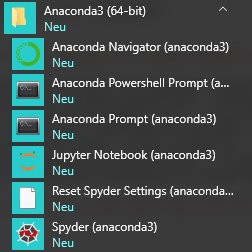
\includegraphics[width=0.5\linewidth]{images/anaconda-shortcuts} \end{center}

You can use \emph{Anaconda Navigator} that allows you to choose a specific programming environment, including \href{https://jupyter.org/}{Jupyter Notebook} that we will use (not JupyterLab, it is more versatile but we want to keep things simple at the beginning!). Alternatively, you can start \emph{Jupyter Notebook} directly from the start menu. Please read the \href{https://jupyter-notebook.readthedocs.io/en/stable/examples/Notebook/examples_index.html}{online documentation} to familiarize yourself with Jupyter Notebook basic interface, e.g.~how to create a new cell, run it, etc.

\hypertarget{install-vs-code}{%
\section*{Installing Visual Studio Code}\label{install-vs-code}}
\addcontentsline{toc}{section}{Installing Visual Studio Code}

\href{https://code.visualstudio.com/}{Visual Studio Code} is a free lightweight open-source editor with strong support for Python. We will start use it in earnest, once our programs grow to be sufficiently long and complex. At the early stages, we will mostly use Jupyter notebooks and I would recommend using Jupyter notebooks using the default browser-based editor you installed as part of \protect\hyperlink{install-anaconda}{Anaconda}. However, you can also work with Jupyter notebooks in VS Code \href{https://code.visualstudio.com/docs/python/jupyter-support}{directly}.

As in case of \protect\hyperlink{install-anaconda}{Anaconda}, download the installer for your platform and follow the instructions. Start VS Code and open any Python file, for example \href{other/empty.py}{this one} (use \texttt{Alt+click} to download it, ignore warnings, it is has only comments, so cannot harm you). When you open Python file for the first time, VS Code will suggest to install a Python extension. Do that and install a linter when VS Code suggests that (\href{https://code.visualstudio.com/docs/python/linting}{linting} highlights syntactical and stylistic problems in your code, making it easier to write consistent clear code).

Once the Python extension is activated, you will see which Python interpreter is used (you can have more than one or you may have multiple \href{https://docs.python.org/3/tutorial/venv.html}{virtual environments}).

\begin{center}
\includegraphics[width=1\linewidth]{images/vscode-python-interpreter} \end{center}

If the selected environment is the wrong one or you are simply not sure, click on it and it will open a drop-down list with all interpreters and environments you have. Consult VS Code \href{https://code.visualstudio.com/docs/python/environments}{online documentation} on environments, if you need to change/add/delete environment (the exact settings may change, so looking at constantly updated online documentation is wiser than copying it here).

\hypertarget{debug-in-vs-code}{%
\section*{Debugging in VIsual Studio Code}\label{debug-in-vs-code}}
\addcontentsline{toc}{section}{Debugging in VIsual Studio Code}

VS Code gives you comprehensive debugging capabilities (read \href{https://code.visualstudio.com/docs/python/python-tutorial}{the tutorial} for detailed information about the tools you have). You can run the code in the debugging mode by pressing on debug button on the left toolbar

\begin{center}
\includegraphics[width=0.05\linewidth]{images/vscode-debug-button} \end{center}

This will open the tab that initially will have the ``Run and Debug'' button or a suggestion to customize the setup

\begin{center}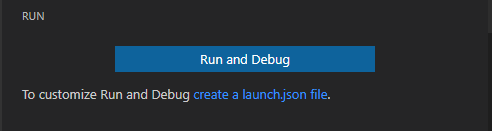
\includegraphics[width=1\linewidth]{images/vscode-rundebug} \end{center}

Click on ``create a launch.json file'', which will open a drop-down list at the top of the editor window:

\begin{center}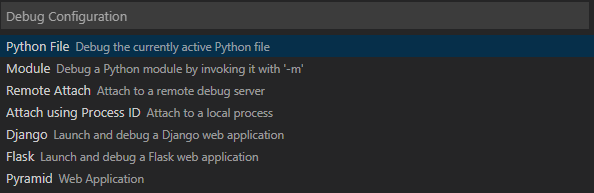
\includegraphics[width=1\linewidth]{images/vscode-debug-options} \end{center}

Pick the first one (Debug the currently active python file) and this will generate a \emph{launch.json} configuration file, which you can close immediately. Now, in an active python file you can press \emph{F5} to start run and debug the program.

\hypertarget{install-psychopy}{%
\section*{Installing PsychoPy}\label{install-psychopy}}
\addcontentsline{toc}{section}{Installing PsychoPy}

This step can wait until the first \protect\hyperlink{memory-game-01}{Memory Game} seminar.

Download and install \href{https://www.psychopy.org/download.html}{Standalone PsychoPy} version. You can install PsychoPy as a conda package or via pip. However, using it as a standalone would ensure that you have all necessary additional libraries and a builder interface for the future use. We will use prepackaged PsychoPy's python environment in \protect\hyperlink{install-vs-code}{VS Code}.

\hypertarget{seminar01}{%
\chapter{Python basics}\label{seminar01}}

Before we start, create a folder called \emph{python-for-experiments} (or with some other more suitable but meaningful name) in you user folder (this is where Anaconda's Jupyter Notebook expects to find them). Download the \href{notebooks/Seminar\%2001.\%20Basics.ipynb}{exercise notebook} and put it in this folder. Open Jupyter Notebook (see \protect\hyperlink{getting-started}{Getting Started}, if you forgot how you do that), navigate to the folder you created and open the downloaded notebook. You will need to switch between explanations here and the exercises in the notebook, so keep them both open.

\hypertarget{variables}{%
\section{Variables}\label{variables}}

The first fundamental concept that we need to be acquainted with is \textbf{variable}. Variables are used to store information and you can think of it as a box with a name tag, so that you can put something into it. The name tag on that box is the name of the variable and its value what you store in it. For example, we can create a variable that stores the number of legs a game character has. We begin with a number typical for a human being.

\begin{center}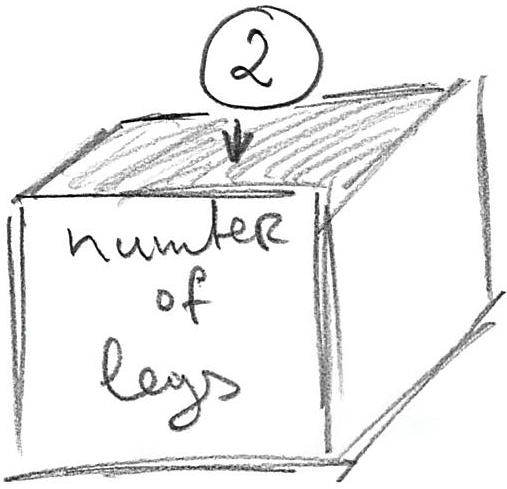
\includegraphics[width=0.5\linewidth]{images/variable-as-box} \end{center}

In Python, you would write

\begin{Shaded}
\begin{Highlighting}[]
\NormalTok{number\_of\_legs }\OperatorTok{=} \DecValTok{2}
\end{Highlighting}
\end{Shaded}

The \textbf{assignment statement} above has very simple structure \texttt{\textless{}variable-name\textgreater{}\ =\ \textless{}value\textgreater{}}. Variable name (name tag on the box) should be meaningful, it can start with letters or \_ and can contain letters, numbers, and \_ symbol but not spaces, tabs, special characters, etc. Python recommends (well, actually, \href{https://www.python.org/dev/peps/pep-0008/}{insists}) that you use \textbf{snake\_case} (all lower-case, underscore for spaces) to format your variable names. The \texttt{\textless{}value\textgreater{}} on the right side is a more complex story, as it can be hard-coded (as in example above), computed using other variables or the same variable, returned by a function, etc.

Using variables means that you can concentrate what corresponding values \textbf{mean} rather than worrying about what these values are. For example, the next time you need to compute something based on number of character's legs (e.g., how many pairs of shoes does a character need), you can compute it based on current value of \texttt{number\_of\_legs} variable rather than assume that it is \texttt{1}.

\begin{Shaded}
\begin{Highlighting}[]
\CommentTok{\# BAD: why 1? Is it because the character has two legs or}
\CommentTok{\# because we issue one pair of shoes per character irrespective of}
\CommentTok{\# their actual number of legs?}
\NormalTok{pairs\_of\_shoes }\OperatorTok{=} \DecValTok{1}

\CommentTok{\# BETTER!}
\NormalTok{pairs\_of\_shoes }\OperatorTok{=}\NormalTok{ number\_of\_legs }\OperatorTok{/} \DecValTok{2}
\end{Highlighting}
\end{Shaded}

Variables also give you flexibility. Their values can change during the program run: player's score is increasing, number of lives decreasing, number of spells it can cast grows or falls depending on their use, etc. Yet, you can always use the value in the variable to perform necessary computations. For example, here is a slightly extended \texttt{number\_of\_shoes} example.

\begin{Shaded}
\begin{Highlighting}[]
\NormalTok{number\_of\_legs }\OperatorTok{=} \DecValTok{2}

\CommentTok{\# ...}
\CommentTok{\# something happens and our character is turned into an octopus}
\NormalTok{number\_of\_legs }\OperatorTok{=} \DecValTok{8}
\CommentTok{\# ...}

\CommentTok{\# the same code still works and we still can compute the correct number of pairs of shoes}
\NormalTok{pairs\_of\_shoes }\OperatorTok{=}\NormalTok{ number\_of\_legs }\OperatorTok{/} \DecValTok{2}
\end{Highlighting}
\end{Shaded}

As noted above, you can think about a variable as a labeled box you can store something in. That means that you can always ``throw away'' the old value and put something new. In case of variables, the ``throwing away'' part happens automatically, as the new value overwrites the old one. Check yourself, what will be final value of the variable in the code below?

\begin{Shaded}
\begin{Highlighting}[]
\NormalTok{number\_of\_legs }\OperatorTok{=} \DecValTok{2}
\NormalTok{number\_of\_legs }\OperatorTok{=} \DecValTok{5}
\NormalTok{number\_of\_legs }\OperatorTok{=} \DecValTok{1}
\NormalTok{number\_of\_legs}
\end{Highlighting}
\end{Shaded}

Do exercise \#1.

As you have already seen, you can \emph{compute} a value instead of specifying it. What would be the answer here?

\begin{Shaded}
\begin{Highlighting}[]
\NormalTok{number\_of\_legs }\OperatorTok{=} \DecValTok{2} \OperatorTok{*} \DecValTok{2}
\NormalTok{number\_of\_legs }\OperatorTok{=} \DecValTok{7} \OperatorTok{{-}} \DecValTok{2}
\NormalTok{number\_of\_legs}
\end{Highlighting}
\end{Shaded}

Do exercise \#2.

\hypertarget{assignments-are-not-equations}{%
\section{Assignments are not equations!}\label{assignments-are-not-equations}}

\textbf{Very important}: although assignments \emph{look} like mathematical equations, they are \textbf{not equations!} Assignments follow a \textbf{very important} rule that you must keep in mind when understanding assignments: the right side expression is evaluated \emph{first} until the final value is computed, then and only then the final value is assigned to the variable specified on the left side (put in the box). What this means is that you can use the same variable on \emph{both} sides! Let's take a look at this code:

\begin{Shaded}
\begin{Highlighting}[]
\NormalTok{x }\OperatorTok{=} \DecValTok{2}
\NormalTok{y }\OperatorTok{=} \DecValTok{5}
\NormalTok{x }\OperatorTok{=}\NormalTok{ x }\OperatorTok{+}\NormalTok{ y }\OperatorTok{{-}} \DecValTok{4}
\end{Highlighting}
\end{Shaded}

What happens when computer evaluates the last line?

\begin{Shaded}
\begin{Highlighting}[]
\NormalTok{x }\OperatorTok{=}\NormalTok{ x }\OperatorTok{+}\NormalTok{ y }\OperatorTok{{-}} \DecValTok{4}
\end{Highlighting}
\end{Shaded}

First, it takes \emph{current} values of all variables (\texttt{2} for \texttt{x} and \texttt{5} for \texttt{y}) and substitutes them into the expression. After that internal step, the expression looks like

\begin{Shaded}
\begin{Highlighting}[]
\NormalTok{x }\OperatorTok{=} \DecValTok{2} \OperatorTok{+} \DecValTok{5} \OperatorTok{{-}} \DecValTok{4}
\end{Highlighting}
\end{Shaded}

Then, it computes the expression on the right side and, \textbf{once the computation is completed}, stores that new value in \texttt{x}

\begin{Shaded}
\begin{Highlighting}[]
\NormalTok{x }\OperatorTok{=} \DecValTok{3}
\end{Highlighting}
\end{Shaded}

Do exercise \#3 to make sure you understand this.

\hypertarget{constants}{%
\section{Constants}\label{constants}}

Although the real power of variables is that you can change their value, you should use them even if the value remains constant. There are no true constants in Python, rather an agreement that their names should be all \texttt{UPPER\_CASE}. Accordingly, when you see \texttt{SUCH\_A\_VARIABLE} you know that you should not change its value. Technically, this is just a recommendation, as no one can stop you from modifying value of a \texttt{CONSTANT}. However, much of Python's ease-of-use comes from such ``gentlemen's agreements'' (such as \texttt{snake\_case} convention above), which you should respect. We will encounter more of them when learning about objects.

Taking all this into account, if number of legs stays constant throughout the game, you should highlight that constancy and write

\begin{Shaded}
\begin{Highlighting}[]
\NormalTok{NUMBER\_OF\_LEGS }\OperatorTok{=} \DecValTok{2}
\end{Highlighting}
\end{Shaded}

I strongly recommend using constants and avoid hardcoding the values. First, if you have several identical values that mean different things (2 legs, 2 eyes, 2 ears, 2 vehicles per character, etc.), seeing a \texttt{2} in the code will not tell you what does this \texttt{2} mean (the legs? the ears? the score multiplier?). You can, of course, figure it out based on the code that uses this number but you could spare yourself that extra effort and use a constant instead. Then, you just read its name and the meaning of the value becomes apparent (and it is the meaning not the actual value that you are mostly interested in). Second, if you decide to \emph{change} that value (say, our main character is now a tripod), when using a constant means you have only one place to worry about, the rest of the code stays as is. If you hard-coded that number, you are in for an exciting (not really) but definitely long search-and-replace throughout the entire code.

Do exercise \#4.

\hypertarget{value-types}{%
\section{Value types}\label{value-types}}

So far, we only used integer numeric values (1, 2, 5, 1000\ldots). Although, Python supports \href{https://docs.python.org/3/library/stdtypes.html}{many different value types}, at first we will concentrate on a small subset of them:

\begin{itemize}
\tightlist
\item
  integer numbers, we already used, e.g.~\texttt{-1}, \texttt{100000}, \texttt{42}.
\item
  float numbers that can take any real value, e.g.~\texttt{42.0}, \texttt{3.14159265359}, \texttt{2.71828}.
\item
  strings that can store text. The text is enclosed between either paired quotes \texttt{"some\ text"} or apostrophes \texttt{\textquotesingle{}some\ text\textquotesingle{}}. This means that you can use quotes or apostrophes inside the string, as long as its is enclosed by the alternative. E.g., \texttt{"students\textquotesingle{}\ homework"} (enclosed in \texttt{"}, apostrophe \texttt{\textquotesingle{}} inside) or \texttt{\textquotesingle{}"All\ generalizations\ are\ false,\ including\ this\ one."\ Mark\ Twain\textquotesingle{}} (quotation enclosed by apostrophes). There is much much more to strings and we will cover that material throughout the course.
\item
  logical / Boolean values that are either \texttt{True} or \texttt{False}.
\end{itemize}

When using a variable it is important that you know what type of value it stores and this is mostly on you. Python will raise an error, if you try doing a computation using incompatible. In some cases, Python will automatically convert values between certain types, e.g.~any integer value is also a real value, so conversion from \texttt{1} to \texttt{1.0} is mostly trivial and automatic. However, in other cases you may need to use explicit conversion. Go to exercise \#5 and try guessing which code will run and which will throw an error due to incompatible types?

\begin{Shaded}
\begin{Highlighting}[]
\DecValTok{5} \OperatorTok{+} \FloatTok{2.0}
\CommentTok{\textquotesingle{}5\textquotesingle{}} \OperatorTok{+} \DecValTok{2}
\CommentTok{\textquotesingle{}5\textquotesingle{}} \OperatorTok{+} \StringTok{\textquotesingle{}2\textquotesingle{}}
\CommentTok{\textquotesingle{}5\textquotesingle{}} \OperatorTok{+} \VariableTok{True}
\DecValTok{5} \OperatorTok{+} \VariableTok{True}
\end{Highlighting}
\end{Shaded}

Do exercise \#5.

Surprised by the last one? This is because internally, \texttt{True} is also \texttt{1} and \texttt{False} is \texttt{0}!

You can explicitly convert from one type to another using special functions. For example, to turn a number or a logical value into a string, you simply write \texttt{str(\textless{}value\textgreater{})}. In examples below, what would be the result?

\begin{Shaded}
\begin{Highlighting}[]
\BuiltInTok{str}\NormalTok{(}\DecValTok{10} \OperatorTok{/} \DecValTok{2}\NormalTok{)}
\BuiltInTok{str}\NormalTok{(}\FloatTok{2.5} \OperatorTok{+} \VariableTok{True}\NormalTok{)}
\BuiltInTok{str}\NormalTok{(}\VariableTok{True}\NormalTok{)}
\end{Highlighting}
\end{Shaded}

Do exercise \#6.

Similarly, you can convert to a logical/Boolean variable using \texttt{bool(\textless{}value\textgreater{})} function. The rules are simple, for numeric values \texttt{0} is \texttt{False}, any other non-zero value is converted to \texttt{True}. For string, an empty string \texttt{\textquotesingle{}\textquotesingle{}} is evaluated to \texttt{False} and non-empty string is converted to \texttt{True}. What would be the output in the examples below?

\begin{Shaded}
\begin{Highlighting}[]
\BuiltInTok{bool}\NormalTok{(}\OperatorTok{{-}}\DecValTok{10}\NormalTok{)}
\BuiltInTok{bool}\NormalTok{(}\FloatTok{0.0}\NormalTok{)}

\NormalTok{secret\_message }\OperatorTok{=} \StringTok{\textquotesingle{}\textquotesingle{}}
\BuiltInTok{bool}\NormalTok{(secret\_message)}

\BuiltInTok{bool}\NormalTok{(}\StringTok{\textquotesingle{}False\textquotesingle{}}\NormalTok{)}
\end{Highlighting}
\end{Shaded}

Do exercise \#7.

Converting to integer or float numbers is trickier. The simplest case is from logical to integer/float, as \texttt{True} gives you \texttt{int(True)} is \texttt{1} and \texttt{float(True)} is \texttt{1.0} and \texttt{False} gives you \texttt{0}/\texttt{0.0}. When converting from float to integer, Python simply drops the fractional part (not rounding!). When converting a string, it must be a valid number of the corresponding type or the error is generated. E.g., you can convert a string like \texttt{"123"} to and integer or a float but this won't work for \texttt{"a123"}. Moreover, you can convert \texttt{"123.4"} to floating-point number but not to an integer, as it has fractional part in it. Given all this, which cells would work and what output would they produce?

\begin{Shaded}
\begin{Highlighting}[]
\BuiltInTok{float}\NormalTok{(}\VariableTok{False}\NormalTok{)}
\BuiltInTok{int}\NormalTok{(}\OperatorTok{{-}}\FloatTok{3.3}\NormalTok{)}
\BuiltInTok{float}\NormalTok{(}\StringTok{"67.8"}\NormalTok{)}
\BuiltInTok{int}\NormalTok{(}\StringTok{"123+3"}\NormalTok{)}
\end{Highlighting}
\end{Shaded}

Do exercise \#8.

\hypertarget{printing-output}{%
\section{Printing output}\label{printing-output}}

To print the value, you need you use \texttt{print()} function (we will talk about functions in general later). In the simplest case, you pass the value and it will be printed out.

\begin{Shaded}
\begin{Highlighting}[]
\BuiltInTok{print}\NormalTok{(}\DecValTok{5}\NormalTok{)}
\end{Highlighting}
\end{Shaded}

\begin{verbatim}
## 5
\end{verbatim}

or

\begin{Shaded}
\begin{Highlighting}[]
\BuiltInTok{print}\NormalTok{(}\StringTok{"five"}\NormalTok{)}
\end{Highlighting}
\end{Shaded}

\begin{verbatim}
## five
\end{verbatim}

Of course, you already know about the variables, so rather than putting a value directly, you can pass a variable instead and its value will be printed out.

\begin{Shaded}
\begin{Highlighting}[]
\NormalTok{number\_of\_pancakes }\OperatorTok{=} \DecValTok{10}
\BuiltInTok{print}\NormalTok{(number\_of\_pancakes)}
\end{Highlighting}
\end{Shaded}

\begin{verbatim}
## 10
\end{verbatim}

or

\begin{Shaded}
\begin{Highlighting}[]
\NormalTok{breakfast }\OperatorTok{=} \StringTok{"pancakes"}
\BuiltInTok{print}\NormalTok{(breakfast)}
\end{Highlighting}
\end{Shaded}

\begin{verbatim}
## pancakes
\end{verbatim}

You can also pass more than one value/variable to the print function and all the values will be printed one after another. For example, if we want to tell the user what did I had for breakfast and just how many of those, we can do

\begin{Shaded}
\begin{Highlighting}[]
\NormalTok{breakfast }\OperatorTok{=} \StringTok{"pancakes"}
\NormalTok{number\_of\_items }\OperatorTok{=} \DecValTok{10}
\BuiltInTok{print}\NormalTok{(breakfast, number\_of\_items)}
\end{Highlighting}
\end{Shaded}

\begin{verbatim}
## pancakes 10
\end{verbatim}

What will be printed by the code below?

\begin{Shaded}
\begin{Highlighting}[]
\NormalTok{dinner }\OperatorTok{=} \StringTok{"stake"}
\NormalTok{count }\OperatorTok{=} \DecValTok{4}
\NormalTok{desert }\OperatorTok{=} \StringTok{"cupcakes"}

\BuiltInTok{print}\NormalTok{(count, dinner, count, desert)}
\end{Highlighting}
\end{Shaded}

Do exercise \#9.

However, you probably would want to be more explicit, when you print out the information. For example, imagine you have these three variables:

\begin{Shaded}
\begin{Highlighting}[]
\NormalTok{meal }\OperatorTok{=} \StringTok{"breakfast"}
\NormalTok{dish }\OperatorTok{=} \StringTok{"pancakes"}
\NormalTok{count }\OperatorTok{=} \DecValTok{10}
\end{Highlighting}
\end{Shaded}

You could, of course do \texttt{print(meal,\ dish,\ count)} but it would be nicer to print ``\emph{I had \textbf{10 pancakes} for \textbf{breakfast}}'', where items in bold would be the inserted variables' values. For this, we need to use string formatting. Please note that the string formatting is not specific to printing, you can create a new string value via formatting and store it in a variable (without printing it out) or print it out (without storing it).

\hypertarget{string-formatting}{%
\section{String formatting}\label{string-formatting}}

A great resource on string formatting in Python is \href{https://pyformat.info/}{pyformat.info}. As Python constantly evolves, it now has more than one way to format strings. Below, I will introduce the ``old'' format that is based on classic string formatting used in \texttt{sprintf} function is C, Matlab, R, and many other programming languages. It is somewhat less flexible than a newer ones but for simple tasks the difference is negligible. Knowing the old format is useful because of its generality. If you want to learn alternatives, read at the link above.

The general call is \texttt{"a\ string\ with\ formatting"\%(tuple\ of\ values\ to\ be\ used\ during\ formatting)}.

In \texttt{"a\ string\ with\ formatting"}, you specify where you want to put the value via \texttt{\%} symbol that is followed by an \emph{optional} formatting info and the \emph{required} symbol that defines the \textbf{type} of the value. The type symbols are

\begin{itemize}
\tightlist
\item
  \texttt{s} for string
\item
  \texttt{d} for an integer
\item
  \texttt{f} for a float value
\item
  \texttt{g} for an ``optimally'' printed float value, so that scientific notation is used for large values (\emph{e.g.}, \texttt{10e5} instead of \texttt{100000}).
\end{itemize}

Here is an example of formatting a string using an integer:

\begin{Shaded}
\begin{Highlighting}[]
\BuiltInTok{print}\NormalTok{(}\StringTok{"I had }\SpecialCharTok{\%d}\StringTok{ pancakes for breakfast"}\OperatorTok{\%}\NormalTok{(}\DecValTok{10}\NormalTok{))}
\end{Highlighting}
\end{Shaded}

\begin{verbatim}
## I had 10 pancakes for breakfast
\end{verbatim}

You are not limited to a single value that you can put into a string. You can specify more locations via \texttt{\%} but you must make sure that you pass the right number of values. Before running it, can you figure out which call will actually work (and what will be the output ) and which will produce an error?

\begin{Shaded}
\begin{Highlighting}[]
\BuiltInTok{print}\NormalTok{(}\StringTok{\textquotesingle{}I had }\SpecialCharTok{\%d}\StringTok{ pancakes and either }\SpecialCharTok{\%d}\StringTok{  or }\SpecialCharTok{\%d}\StringTok{ stakes for dinner\textquotesingle{}}\OperatorTok{\%}\NormalTok{(}\DecValTok{2}\NormalTok{))}
\BuiltInTok{print}\NormalTok{(}\StringTok{\textquotesingle{}I had }\SpecialCharTok{\%d}\StringTok{ pancakes and }\SpecialCharTok{\%d}\StringTok{ stakes for dinner\textquotesingle{}}\OperatorTok{\%}\NormalTok{(}\DecValTok{7}\NormalTok{, }\DecValTok{10}\NormalTok{))}
\BuiltInTok{print}\NormalTok{(}\StringTok{\textquotesingle{}I had }\SpecialCharTok{\%d}\StringTok{ pancakes and }\SpecialCharTok{\%d}\StringTok{ stakes for dinner\textquotesingle{}}\OperatorTok{\%}\NormalTok{(}\DecValTok{1}\NormalTok{, }\DecValTok{7}\NormalTok{, }\DecValTok{10}\NormalTok{))}
\end{Highlighting}
\end{Shaded}

Do exercise \#10.

In case of real values you have two options: \texttt{\%f} and \texttt{\%g}. The latter uses scientific notation (e.g.~\texttt{1e10} for \texttt{10000000000}) to make a representation more compact.

Do exercise \#11 to get a better feeling for the difference.

These is much more to formatting and you can read about it at \href{https://pyformat.info/}{pyformat.info}. However, these basics are sufficient for us to start programming our first game during the next seminar. Don't forget to submit your exercise notebook and see you next time!

\hypertarget{seminar02}{%
\chapter{Guess the Number}\label{seminar02}}

Seminar \#1 covered Python basics, so now you are ready to start developing you first game! We will build it step by step and there will be a lot to learn about input, libraries, conditional statements, and indentation. As before, download \href{notebooks/Seminar\%2002.\%20Guess\%20the\%20number.ipynb}{exercise notebook}, copy it in your designated folder, and open it in Jupyter Notebook.

\hypertarget{game-description}{%
\section{Game description}\label{game-description}}

We will program a game in which one participant (computer) picks the number within a certain range (say, between 1 and 10) and the other participant (player) is trying to guess it. After every guess, the first participant (computer) responds whether the actual number is lower than a guess, higher than a guess, or matches it. The game is over when the player correctly guess the number or (in the later version of the game) runs out of attempts.

Our first version will allow just one attempt (will make it more fun later on) and the overall game algorithm will look like this:

\begin{Shaded}
\begin{Highlighting}[]
\CommentTok{\# 1. computer generates a random number}
\CommentTok{\# 2. prints it out for debug purposes}
\CommentTok{\# 3. prompts user to enter a guess}
\CommentTok{\# 4. compares two numbers and print outs the outcome}
\CommentTok{\#    "My number is lower", "My number is higher", or "Spot on!"}
\end{Highlighting}
\end{Shaded}

\hypertarget{lets-pick-the-number-exercise-1}{%
\section{Let's pick the number (Exercise 1)}\label{lets-pick-the-number-exercise-1}}

Let us start by creating a variable that will hold a number that computer ``picked''. Let us name it \texttt{number\_picked} (you can some other meaningful name as well but it might be easier if we all stick to the same name). To make things a bit simpler at the beginning, let us assign some hard=coded arbitrary number between 1 and 10 to it (whatever you fill like). Then, let us print it out, so that we know the number ourselves (we know it now but that won't be the case when computer will generate it randomly). Use string formatting to make things user-friendly, e.g., print out something like ``The number I've picked is \ldots{}''. Your code should be a two-liner:

\begin{Shaded}
\begin{Highlighting}[]
\CommentTok{\# 1. create variable and set it value}
\CommentTok{\# 2. print out the value}
\end{Highlighting}
\end{Shaded}

Put your code into exercise \#1 and make sure your code works!.

\hypertarget{input-function}{%
\section{Asking user for a guess (Exercise 2)}\label{input-function}}

Now we need to ask the player to enter their guess. For this, we will use \href{https://docs.python.org/3/library/functions.html\#input}{input({[}prompt{]})} function (here and below the links lead to the official documentation). It prints out \texttt{prompt} (a string) if you supplied it, reads the input (key presses) until the user presses \texttt{Enter}, and returns it \textbf{as a string}. For a moment, let us assume that the input is always an valid integer number (so, type only valid integers!), so we can convert it to an integer without extra checks (will add them later) and assign this value to a new variable called \texttt{guess}. Thus, you need to write a single line assignment statement with \texttt{guess} variable on the left side, whereas on the right should be a call to the \texttt{input(...)} function (think of a nice prompt message) wrapped by the type-conversion to \texttt{int(...)}. Switch to exercise 2 and, for the moment, only enter valid integers when running the code, so that the conversion works without an error.

Put your code into exercise \#2.

\hypertarget{conditional-if-statement}{%
\section{\texorpdfstring{Conditional \emph{if} statement}{Conditional if statement}}\label{conditional-if-statement}}

Now we have two numbers: One that computer picked and one that is player's guess. Now, we need to compare them to provide correct output message. For this, we will use conditional \href{https://docs.python.org/3/tutorial/controlflow.html\#if-statements}{if statement}:

\begin{Shaded}
\begin{Highlighting}[]
\ControlFlowTok{if}\NormalTok{ some\_condition\_is\_true:}
    \CommentTok{\# do something}
\ControlFlowTok{elif}\NormalTok{ some\_other\_condition\_is\_true:}
    \CommentTok{\# do something else}
\ControlFlowTok{elif}\NormalTok{ yet\_another\_condition\_is\_true:}
    \CommentTok{\# do yet something else}
\ControlFlowTok{else}\NormalTok{:}
    \CommentTok{\# do something only if all conditions above are false.}
\end{Highlighting}
\end{Shaded}

Only the \texttt{if} part is required, whereas \texttt{elif} (short for ``else, if'') and \texttt{else} are optional. Thus you can do something, only if a condition is true:

\begin{Shaded}
\begin{Highlighting}[]
\ControlFlowTok{if}\NormalTok{ some\_condition\_is\_true:}
    \CommentTok{\# do something, but OTHERWISE DO NOT DO ANYTHING }
    \CommentTok{\# and continue with code execution}
  
\CommentTok{\# some code that is executed after the if{-}statement,}
\CommentTok{\# irrespective of whether the condition was true or not.}
\end{Highlighting}
\end{Shaded}

Before we can properly use conditional statements, you need to understand (1) the conditions themselves and (2) use of indentation as a mean of grouping statements together.

\hypertarget{conditions-and-comparisons-exercises-3-8}{%
\section{Conditions and comparisons (exercises 3-8)}\label{conditions-and-comparisons-exercises-3-8}}

Condition is any expression that can be evaluated to see whether it is \texttt{True} or \texttt{False}. A straightforward example of such expression are comparisons, in human language expressed as ``is today Thursday?'', ``is the answer equal to 42'', ``is it raining and I have an umbrella?''. We will concentrate on them here but later you will see that in Python \textbf{any} expression is either \texttt{True} or \texttt{False}, even when it does not look like a comparison.

For the comparison, you can use the following operators:

\begin{itemize}
\tightlist
\item
  \emph{``A is equal B''} is written as \texttt{A\ ==\ B}.
\item
  \emph{``A is not equal B''} is written as \texttt{A\ !=\ B}.
\item
  \emph{``A is greater than B''} and \emph{``A is smaller than B''} are, respectively, \texttt{A\ \textgreater{}\ B} and \texttt{A\ \textless{}\ B}.
\item
  \emph{``A is greater than or equal to B''} and \emph{``A is smaller than or equal to B''} are, respectively, \texttt{A\ \textgreater{}=\ B} and \texttt{A\ \textless{}=\ B} (please note the order of symbols!).
\end{itemize}

Go to exercise \#3 to solve some comparisons.

You can \emph{invert} the logical value using \texttt{not} operator, as \texttt{not\ True} is \texttt{False} and \texttt{not\ False} is \texttt{True}. This means that \texttt{A\ !=\ B} is the same as \texttt{not\ A\ ==\ B} and, correspondingly, \texttt{A\ ==\ B} is \texttt{not\ A\ !=\ B}. To see how that works, consider both cases when \texttt{A} is indeed equal \texttt{B} and when it is not.

\begin{itemize}
\tightlist
\item
  If A is equal B then \texttt{A\ ==\ B} evaluates to \texttt{True}. The \texttt{A\ !=\ B} is then \texttt{False}, so \texttt{not\ A\ !=\ B} → \texttt{not\ False} → \texttt{True}.
\item
  If A is not equal B then \texttt{A\ ==\ B} evaluates to \texttt{False}. The \texttt{A\ !=\ B} is then \texttt{True}, so \texttt{not\ A\ !=\ B} → \texttt{not\ True} → \texttt{False}.
\end{itemize}

Go to exercise \#4 to explore this inversion yourself.

You can also combine several comparisons using \texttt{and} and/or \texttt{or} operators. As in human language, \texttt{and} means that both parts must be true: \texttt{True\ and\ True} → \texttt{True} but \texttt{True\ and\ False} → \texttt{False}, \texttt{False\ and\ True} → \texttt{False}, and \texttt{False\ and\ False} → \texttt{False}. Same holds if you have more have than two conditions/comparisons, \textbf{all} of them must be true. In case of \texttt{or} only one of the statements must be true, e.g.~\texttt{True\ and\ True} → \texttt{True}, \texttt{True\ and\ False} → \texttt{True}, \texttt{False\ and\ True} → \texttt{True}, but \texttt{False\ and\ False} → \texttt{False}. Again, for more than two comparisons/conditions at least one of them should be true for the entire expression to be true.

Do exercises \#5 and \#6.

Subtle but important point: conditions are evaluated from left to right until the whole expression can be definitely resolved. This means that if the first expression in a \texttt{and} pair is \texttt{False}, the second one is \textbf{never evaluated}. I.e., if \texttt{first\ and\ second} expressions both need to be \texttt{True} and you know that already \texttt{first} expression is false, the whole expression will be \texttt{False} in any case. This means that in the code below there will be no error, even though evaluating \texttt{int("e123")} raises \texttt{ValueError}.

\begin{Shaded}
\begin{Highlighting}[]
\DecValTok{2} \OperatorTok{*} \DecValTok{2} \OperatorTok{==} \DecValTok{5} \KeywordTok{and} \BuiltInTok{int}\NormalTok{(}\StringTok{"e123"}\NormalTok{) }\OperatorTok{==} \DecValTok{123}
\end{Highlighting}
\end{Shaded}

However, reverse the order, so that \texttt{int("e123")\ ==\ 123} needs to be evaluated first and you get the error message

\begin{Shaded}
\begin{Highlighting}[]
\BuiltInTok{int}\NormalTok{(}\StringTok{"e123"}\NormalTok{) }\OperatorTok{==} \DecValTok{123} \KeywordTok{and} \DecValTok{2} \OperatorTok{*} \DecValTok{2} \OperatorTok{==} \DecValTok{4}
\CommentTok{\# Generates ValueError: invalid literal for int() with base 10: \textquotesingle{}e123\textquotesingle{}}
\end{Highlighting}
\end{Shaded}

Similarly, if \emph{any} expression in \texttt{or} is \texttt{True}, you do not need to check the rest.

\begin{Shaded}
\begin{Highlighting}[]
\DecValTok{2} \OperatorTok{*} \DecValTok{2} \OperatorTok{==} \DecValTok{4} \KeywordTok{or} \BuiltInTok{int}\NormalTok{(}\StringTok{"e123"}\NormalTok{) }\OperatorTok{==} \DecValTok{123}
\end{Highlighting}
\end{Shaded}

However, if the first condition is \texttt{False}, we do need to continue (and stumble into an error):

\begin{Shaded}
\begin{Highlighting}[]
\DecValTok{2} \OperatorTok{*} \DecValTok{2} \OperatorTok{==} \DecValTok{5} \KeywordTok{or} \BuiltInTok{int}\NormalTok{(}\StringTok{"e123"}\NormalTok{) }\OperatorTok{==} \DecValTok{123}
\CommentTok{\# Generates ValueError: invalid literal for int() with base 10: \textquotesingle{}e123\textquotesingle{}}
\end{Highlighting}
\end{Shaded}

Do exercise \#7.

Finally, like in simple arithmetic, you can use brackets \texttt{()} to group conditions together. Thus a statement ``I always eat chocolate but I eat spinach only when I am hungry'' can be written as \texttt{food\ ==\ "chocolate"\ or\ (food\ ==\ "spinach"\ and\ hungry)}. Here, \texttt{the\ food\ ==\ "chocolate"} and \texttt{food\ ==\ "spinach"\ and\ hungry} are evaluated independently, their values are substituted in their place and then the \texttt{and} condition is evaluated.

Do exercise \#8.

\hypertarget{grouping-statements-via-identation-exercise-9}{%
\section{Grouping statements via identation (exercise \#9)}\label{grouping-statements-via-identation-exercise-9}}

Let us go back to the conditional if-statement. Take a look at following code example, in which statement \#1 is executed only if some condition is true, whereas statement \#2 is executed after that irrespective of the condition.

\begin{Shaded}
\begin{Highlighting}[]
\ControlFlowTok{if}\NormalTok{ some\_condition\_is\_true:}
\NormalTok{    statement }\CommentTok{\#1}
\NormalTok{statement }\CommentTok{\#2 }
\end{Highlighting}
\end{Shaded}

Both statements \#1 and \#2 appear after the if-statement, so how does Python now that the first one is executed only if condition is true but the other one always runs? The answer is indentation (the \textbf{4 (four!)} spaces, they are automatically added whenever you press \texttt{Tab} and removed whenever you press \texttt{Shift\ +\ Tab}) that puts statement \#1 \emph{inside} the if-statement. Thus, indentation shows whether statements belong to the same group (same indentation as for \texttt{if} and \texttt{statement\ \#2}) or are inside conditional statement, loop, or function (\texttt{statement\ \#1}). For more complex code that will have, for example, if-statement inside an if-statement inside a loop, you will express this by adding more levels of indentation. E.g.

\begin{Shaded}
\begin{Highlighting}[]
\CommentTok{\# some statements outside of the loop (0 indentation)}
\ControlFlowTok{while}\NormalTok{ game\_is\_not\_over: }\CommentTok{\# (0 indentation)}
    \CommentTok{\# statements inside of the loop }
    \ControlFlowTok{if}\NormalTok{ key\_pressed: }\CommentTok{\# (indentation of 4)}
        \CommentTok{\# inside loop and if{-}statement }
        \ControlFlowTok{if}\NormalTok{ key }\OperatorTok{==} \StringTok{"Space"}\NormalTok{: }\CommentTok{\# (indentation of 8)}
            \CommentTok{\# inside the loop, and if{-}statement, and another if{-}statement}
\NormalTok{            jump() }\CommentTok{\# (indentation of 12)}
        \ControlFlowTok{else}\NormalTok{: }\CommentTok{\# (indentation of 4)}
            \CommentTok{\# inside the loop, and if{-}statement, and else part of another if{-}statement}
\NormalTok{            stand() }\CommentTok{\# (indentation of 12)}
    
    \CommentTok{\# statements inside of the loop but outside of the outermost if{-}statement}
    \BuiltInTok{print}\NormalTok{(key) }\CommentTok{\# (indentation of 4)}
    
\CommentTok{\# some statements outside of the loop (0 indentation)}
\end{Highlighting}
\end{Shaded}

Pay very close attention to the indentation as it determines which statements are executed together!

Do exercise \#9.

The \texttt{if} and \texttt{ifelse} statements are evaluated until one of them turns out to be \texttt{True}. After that any following \texttt{ifelse} and \texttt{else} statements are simply ignored.

Do exercise \#10.

\hypertarget{checking-the-answer-exercise-11}{%
\section{Checking the answer (Exercise 11)}\label{checking-the-answer-exercise-11}}

Now you have all necessary instruments to finish the first version of our game. Go to exercise \#11 and, first, copy-paste your solutions to exercise \#1 (settings computer pick and printing it out) and \#2 (getting player input as an integer). Now, add conditional statements below, so that

\begin{itemize}
\tightlist
\item
  if the computer pick is smaller than player's guess, it will print \texttt{"My\ number\ is\ lower!"}
\item
  if the computer pick is larger than player's guess, it will print \texttt{"My\ number\ is\ higher!"}
\item
  if two numbers are identical, it will print \texttt{"Spot\ on!"}
\end{itemize}

Put your code into exercise \#11.

\hypertarget{picking-number-randomly-exercise-12}{%
\section{Picking number randomly (Exercise 12)}\label{picking-number-randomly-exercise-12}}

Our game is ``feature-complete'': computer picks a number, player makes a guess, computer responds appropriately. However, currently we are playing for both sides, as we hand pick the number for computer. Now, we will let computer pick this number itself using \href{https://docs.python.org/3/library/random.html\#random.randint}{randint(a, b)} function. It is part of the \href{https://docs.python.org/3/library/random.html}{random} library, so you will need to \emph{import} it first. We will talk about libraries and importing them in greater detail later. For now, it suffices that the top line of your code is

\begin{Shaded}
\begin{Highlighting}[]
\ImportTok{from}\NormalTok{ random }\ImportTok{import}\NormalTok{ randint}
\end{Highlighting}
\end{Shaded}

Function \texttt{randint(a,\ b)} generates a random integer on the interval \texttt{a..b}. In our case, this interval is \texttt{1..10}. Go to exercise \#11. First copy-paste your solution for exercise \#12. Add the \texttt{from\ random\ import\ randint} as the first line. Then, replace the hard-coded value you used for computer's pick with a call to \texttt{randint()} function. Run the code several times to check that computer does pick different random values.

Put your code into exercise \#12.

Congratulations, you just programmed your first computer game! Yes, it is very simple but it has key ingredients: a random decision by computer, user input, and feedback. Next time, you will learn about loops to allow for multiple attempts and about functions to make your code modular and reliable. In the meantime, let us solidify your knowledge by programming yet another game!

\hypertarget{one-armed-bandit-exercise-13}{%
\section{One-armed bandit (Exercise 13)}\label{one-armed-bandit-exercise-13}}

You know everything you need to program a simple version of an ``one-armed bandit'' game (exercise \#13). Here is the game logic:

\begin{enumerate}
\def\labelenumi{\arabic{enumi}.}
\tightlist
\item
  \texttt{from\ random\ import\ randint}
\item
  Generate three random integers (say, between 1 and 5) and store them in three variables \texttt{slot1}, \texttt{slot2}, and \texttt{slot3}.
\item
  Print out the numbers, use string formatting to make it look nice.
\item
  In addition,

  \begin{itemize}
  \tightlist
  \item
    if all three values are the same, print \texttt{"Three\ of\ a\ kind!"}.
  \item
    If only two numbers match, print \texttt{"Pair!"}.
  \item
    Print nothing, if all numbers are different.
  \end{itemize}
\end{enumerate}

Put your code into exercise \#13.

\hypertarget{seminar03}{%
\chapter{Guess the Number, the Sequel}\label{seminar03}}

During our previous seminar, you programmed a single-attempt-only ``Guess the Number'' game. Now, you will expand to multiple attempts and will add other bells-and-whistles to make it more fun. Download the \href{notebooks/Seminar\%2003.\%20Guess\%20the\%20number,\%20part\%202.ipynb}{exercise notebook} before we start!

\hypertarget{while-loop}{%
\section{While loop (Exercises 1-2)}\label{while-loop}}

If you want to repeat something, you need to use loops. There are two types of loops: \href{https://wiki.python.org/moin/WhileLoop}{while} loop, which is repeated \emph{while} a condition is true, and \href{https://wiki.python.org/moin/ForLoop}{for} loop that iterates over items (we will use it later).

The basic structure of a \emph{while} loop is

\begin{Shaded}
\begin{Highlighting}[]
\CommentTok{\# statements before the loop}

\ControlFlowTok{while} \OperatorTok{\textless{}}\NormalTok{condition}\OperatorTok{\textgreater{}}\NormalTok{:}
    \CommentTok{\# statements inside are executed}
    \CommentTok{\# repeatedly for as long as}
    \CommentTok{\# the condition is True}
    
\CommentTok{\# statements after the loop}
\end{Highlighting}
\end{Shaded}

The \texttt{\textless{}condition\textgreater{}} here is any expression that is evaluated to be either \texttt{True} or \texttt{False}, just like in an \emph{if-elif-else} conditional statement.

Do exercise \#1.

Let us use \emph{while} loop, so that the player keeps guessing until finally getting it right. You can copy-paste the code you programmed during the last seminar or could redo it from scratch (I would strongly recommend you doing the latter!). The overall program structure should be the following

\begin{Shaded}
\begin{Highlighting}[]
\ImportTok{from}\NormalTok{ random }\ImportTok{import}\NormalTok{ randint}

\CommentTok{\# generated random number and store in computer\_pick variable}
\CommentTok{\# print it out for debugging purposes}
\CommentTok{\# get player input, convert it to an integer, and store}

\CommentTok{\# while \textless{}players guess is not equal to the value the computer picked\textgreater{}:}
    \CommentTok{\# print out "my number is smaller" or "my number is larger" using if{-}else statement}
    
\CommentTok{\# print "Spot on!" (because if we got here that means guess is equal to the computer\textquotesingle{}s pick)}
\end{Highlighting}
\end{Shaded}

Put your code into exercise \#2.

\hypertarget{counting-attempts-exercise-3}{%
\section{Counting attempts (Exercise \#3)}\label{counting-attempts-exercise-3}}

Now let us add a variable that will count the total number of attempts the player required. For this, create a new variable (call it \texttt{attempts} or something similar) \emph{before the loop} and initialize it \texttt{0}. Add \texttt{1} to it every time the player inputs the guess. After the loop, expand the \texttt{"Spot\ on!"} message you print out by adding information about the attempts count. Use string formatting to make things look nice, e.g.~\texttt{"Spot\ on,\ you\ needed\ 5\ attempts"}.

Put your code into exercise \#3.

\hypertarget{break}{%
\section{Breaking (and exiting, Exercise \#4)}\label{break}}

\emph{While} loop is continuously executed while the condition is \texttt{True} and, importantly, all code inside is executed before the condition is evaluated again. However, sometimes you may need to abort sooner without executing the remaining code. For this, Python gives you a \texttt{break} statement that causes the program to exit the loop immediately and to continue with the code after the loop.

\begin{Shaded}
\begin{Highlighting}[]
\CommentTok{\# this code runs before the loop}

\ControlFlowTok{while} \OperatorTok{\textless{}}\NormalTok{somecondition}\OperatorTok{\textgreater{}}\NormalTok{:}
  \CommentTok{\# this code runs on every iteration}
  
    \ControlFlowTok{if} \OperatorTok{\textless{}}\NormalTok{someothercondition}\OperatorTok{\textgreater{}}\NormalTok{:}
        \ControlFlowTok{break}
  
  \CommentTok{\# this code runs on every iteration but not when you break out of the loop}

\CommentTok{\# this code runs after the loop}
\end{Highlighting}
\end{Shaded}

Do exercise \#4 to build the intuition.

\hypertarget{limiting-number-of-attempts-via-break-exercise-5}{%
\section{Limiting number of attempts via break (Exercise 5)}\label{limiting-number-of-attempts-via-break-exercise-5}}

Let's put the player under some pressure! Decide on maximal number of attempts allowed and stores in a constant. Pick an appropriate name (e.g.~\texttt{MAX\_ATTEMPTS}) and REMEMBER, ALL CAPITAL LETTERS for a constant name! Now, use \texttt{break} to quit the \texttt{while} loop, if current attempt number is greater than \texttt{MAX\_ATTEMPTS}.

Put your code into exercise \#5.

\hypertarget{correct-end-of-game-message-exercise-6}{%
\section{Correct end-of-game message (Exercise 6)}\label{correct-end-of-game-message-exercise-6}}

Think about the final message. Currently it says ``Spot on\ldots{}'' because we assumed that you exited the loop because you gave the correct answer. With limited attempts that is not the case, as the player could out of the loop because

\begin{enumerate}
\def\labelenumi{\arabic{enumi}.}
\tightlist
\item
  They answered correctly
\item
  They ran out of attempts.
\end{enumerate}

Use \texttt{if-else} conditional statement to print out an appropriate message (e.g., \texttt{"Better\ luck\ next\ time!}, if the player lost).

Put your code into exercise \#6.

\hypertarget{limiting-number-of-attempts-with-a-break-exercise-7}{%
\section{Limiting number of attempts with a break (Exercise 7)}\label{limiting-number-of-attempts-with-a-break-exercise-7}}

Modify your code to work without \texttt{break} statement. Modify your condition so that loop repeats while player's guess is incorrect and the number of attempts is still less than the maximally allowed.

Put your code into exercise \#7.

\hypertarget{show-remaining-attempts-exercise-8}{%
\section{Show remaining attempts (Exercise 8)}\label{show-remaining-attempts-exercise-8}}

Modify the \texttt{input} prompt message to include number of \emph{remaining} attempts. E.g. \texttt{"Please\ enter\ the\ guess,\ you\ have\ X\ attempts\ remaining"}.

Put your code into exercise \#8.

\hypertarget{repeating-the-game-exercise-9}{%
\section{Repeating the game (Exercise 9)}\label{repeating-the-game-exercise-9}}

Let us an option for the player to play again. This means putting \emph{all} the current code inside of another \texttt{while} loop that is repeated for as long as the player wants to play. The code should look following:

\begin{Shaded}
\begin{Highlighting}[]
\ImportTok{from}\NormalTok{ random }\ImportTok{import}\NormalTok{ randint}

\CommentTok{\# define MAX\_ATTEMPTS}

\CommentTok{\# define a variable called "want\_to\_play" and set to True}
\ControlFlowTok{while}\NormalTok{ want\_to\_play:}
  \CommentTok{\# your working game code goes here ()}
  
  \CommentTok{\# ask user whether via input function. E.g. "Want to play again? Y/N"}
  \CommentTok{\# want\_to\_play should be True if user input is equal to "Y"}
  
\CommentTok{\# very final message, e.g. "Thank you for playing the game!"}
\end{Highlighting}
\end{Shaded}

\textbf{Pay extra attention to indentation to group the code properly!}

Put your code into exercise \#9.

\hypertarget{best-score-exercise-10}{%
\section{Best score (Exercise 10)}\label{best-score-exercise-10}}

A ``proper'' game typically keeps the track of players' performance. Let us record what was the fewest number of attempts that the player needed to guess the number. For this, create a new variable \texttt{fewest\_attempts} and set it to \texttt{MAX\_ATTEMPTS} (this is as bad as the player can be). Think, where do you need to create it? Once a game round is over and you know how many attempts the player required, update it if the number of attempts that the player used was \emph{less} than the current value. You can add the information about ``Best so far'' into the game-round-over message.

Put your code into exercise \#10.

\hypertarget{counting-game-rounds-exercise-11}{%
\section{Counting game rounds (Exercise 11)}\label{counting-game-rounds-exercise-11}}

Let us count how many rounds the player played. The idea and implementation is the same as with counting the attempts. Create a new variable, initialize it to 0, increment by 1 whenever a new round starts. Include the total number of rounds into the very final message, e.g.~``Thank you for playing the game X times!''

Put your code into exercise \#11.

\hypertarget{wrap-up}{%
\section{Wrap up}\label{wrap-up}}

Most excellent, you now have a proper working computer game with game rounds, limited attempts, best score, and what not!

\hypertarget{seminar04}{%
\chapter{Hunt the Wumpus, part 1}\label{seminar04}}

We will program text adventure computer game \href{https://en.wikipedia.org/wiki/Hunt_the_Wumpus}{Hunt the Wumpus}: ``In the game, the player moves through a series of connected caves, arranged in a dodecahedron, as they hunt a monster named the Wumpus. The turn-based game has the player trying to avoid fatal bottomless pits and''super bats" that will move them around the cave system; the goal is to fire one of their ``crooked arrows'' through the caves to kill the Wumpus\ldots"

As before, we will start with a very basic program and will build it step-by-step towards the final version. Don't forget to download the \href{notebooks/Seminar\%2004.\%20Hunt\%20the\%20Wumpus,\%20part\%201.ipynb}{exercise notebook}.

\hypertarget{lists}{%
\section{Lists}\label{lists}}

So far, we were using variables to store single values: computer's pick, player's guess, number of attempts, etc. However, you can store multiple values in a variable using \href{https://docs.python.org/3/library/stdtypes.html\#list}{lists}. The idea is fairly straightforward, a variable is not a simple box but a box with slots for values numbered from \texttt{0} to \texttt{len(variable)-1}.

The list is defined via square brackets \texttt{\textless{}variable\textgreater{}\ =\ {[}\textless{}value1\textgreater{},\ \textless{}value2\textgreater{},\ ...\ \textless{}valueN\textgreater{}{]}} and an individual value can be accessed also via square brackets \texttt{\textless{}variable\textgreater{}{[}\textless{}index\textgreater{}{]}} where index goes from \texttt{0} to \texttt{len(\textless{}variable\textgreater{})-1} (\href{https://docs.python.org/3/library/functions.html\#len}{\texttt{len(\textless{}object\textgreater{})}} function returns number of items in an object, in our case, it would be a list). Thus, if you have five values in the list, the index of the first one is \texttt{0} (not \texttt{1}) and the index of the last one is \texttt{4} (not \texttt{5})!

Do exercise \#1 see how lists are defined and indexed.

You can also get many values from the list via so called \emph{slicing} when you specify index of many elements via \texttt{\textless{}start\textgreater{}:\textless{}stop\textgreater{}}. There is a catch though and, as this is a recurrent theme in Python, pay close attention: The index slicing builds goes from \texttt{start} up to \textbf{but not including} \texttt{stop}, in mathematical notation \([start, stop)\). So, if you have a list \texttt{my\_pretty\_numbers} that holds five values and you want to get values from second (index \texttt{1}) till fourth (index \texttt{3}) you need to write the slice as \texttt{1:4} (not \texttt{1:3}!). This \emph{including the start but excluding the stop} is both fairly counterintuitive (I still have to consciously remind myself about this) and widely used in Python.

Do exercise \#2 to build the intuition.

You can also omit either \texttt{start} or \texttt{stop}. In this case, Python will assume that a missing \texttt{start} means \texttt{0} (the index of the first element) and missing \texttt{stop} means \texttt{len(\textless{}list\textgreater{})}. If you omit \emph{both}, e.g., \texttt{my\_pretty\_numbers{[}:{]}} it will return all values, as this is equivalent to \texttt{my\_pretty\_numbers{[}0:len(my\_pretty\_numbers){]}}.\footnote{Note, that this is almost but not quite the same thing as just writing \texttt{my\_pretty\_numbers}, the difference is subtle but important and we will look into it later when talking about mutable versus immutable types.}

Do exercise \#3.

You can also use \emph{negative} indexes that are relative to length of the list. Thus, if you want to get the \emph{last} element of the list, you can say \texttt{my\_pretty\_numbers{[}len(my\_pretty\_numbers)-1{]}} or just \texttt{my\_pretty\_numbers{[}-1{]}}. The last-but-one element would be \texttt{my\_pretty\_numbers{[}-2{]}}, etc. You can use negative indexes for slicing but keep in mind \emph{including the start but excluding the stop}: \texttt{my\_pretty\_numbers{[}:-1{]}} will return all but last element of the list not the entire list.

Do exercise \#4.

The slicing can be extended by specifying a \texttt{step}, so that \texttt{stop:start:step}. This can be combined with omitted and negative indexes. To get every \emph{odd} element of the list, you write \texttt{my\_pretty\_numbers{[}::2{]}}:

\begin{Shaded}
\begin{Highlighting}[]
\NormalTok{my\_pretty\_numbers }\OperatorTok{=}\NormalTok{ [}\DecValTok{1}\NormalTok{, }\DecValTok{2}\NormalTok{, }\DecValTok{3}\NormalTok{, }\DecValTok{4}\NormalTok{, }\DecValTok{5}\NormalTok{, }\DecValTok{6}\NormalTok{, }\DecValTok{7}\NormalTok{]}
\NormalTok{my\_pretty\_numbers[::}\DecValTok{2}\NormalTok{]}
\end{Highlighting}
\end{Shaded}

\begin{verbatim}
## [1, 3, 5, 7]
\end{verbatim}

Do exercise \#5.

Finally, for those who are familiar with R, the good news is that Python does not allow you to use indexes outside of the range, so trying to get 6\textsuperscript{th} element (index \texttt{5}) of a five-element-long list will generate a simple and straightforward error (a so-called \href{https://en.wikipedia.org/wiki/Fail-fast}{fail-fast} principle). The bad news is that if your \emph{slice} is larger than the range, it will truncated to the range without an extra warning or an error. So, for a five-element list \texttt{my\_pretty\_numbers{[}:6{]}} will return all numbers of to the maximal possible index (thus, effectively, this is equivalent to \texttt{my\_pretty\_numbers{[}:{]}}). Moreover, if the slice is empty (\texttt{2:2}, cannot include \texttt{2}, even though it starts from it) or the entire slice is outside of the range, Python will return an empty list, again, neither warning or error is generated.

Do exercise \#6.

\hypertarget{caves}{%
\section{Caves}\label{caves}}

In our game, the player will wander through a systems of caves with cave being connected to three other caves. The cave layout will be \emph{CONSTANT}, so we will define at the beginning of the program as follows.

\begin{Shaded}
\begin{Highlighting}[]
\NormalTok{CAVES }\OperatorTok{=}\NormalTok{ [[}\DecValTok{1}\NormalTok{, }\DecValTok{4}\NormalTok{, }\DecValTok{5}\NormalTok{], [}\DecValTok{2}\NormalTok{, }\DecValTok{0}\NormalTok{, }\DecValTok{7}\NormalTok{], [}\DecValTok{3}\NormalTok{, }\DecValTok{1}\NormalTok{, }\DecValTok{9}\NormalTok{], [}\DecValTok{4}\NormalTok{, }\DecValTok{2}\NormalTok{, }\DecValTok{11}\NormalTok{], }
\NormalTok{         [}\DecValTok{0}\NormalTok{, }\DecValTok{3}\NormalTok{, }\DecValTok{13}\NormalTok{], [}\DecValTok{6}\NormalTok{, }\DecValTok{14}\NormalTok{, }\DecValTok{0}\NormalTok{], [}\DecValTok{7}\NormalTok{, }\DecValTok{5}\NormalTok{, }\DecValTok{15}\NormalTok{], [}\DecValTok{8}\NormalTok{, }\DecValTok{6}\NormalTok{, }\DecValTok{1}\NormalTok{], }
\NormalTok{         [}\DecValTok{9}\NormalTok{, }\DecValTok{7}\NormalTok{, }\DecValTok{16}\NormalTok{], [}\DecValTok{10}\NormalTok{, }\DecValTok{8}\NormalTok{, }\DecValTok{2}\NormalTok{], [}\DecValTok{11}\NormalTok{, }\DecValTok{9}\NormalTok{, }\DecValTok{17}\NormalTok{], [}\DecValTok{12}\NormalTok{, }\DecValTok{10}\NormalTok{, }\DecValTok{3}\NormalTok{], }
\NormalTok{         [}\DecValTok{13}\NormalTok{, }\DecValTok{11}\NormalTok{, }\DecValTok{18}\NormalTok{], [}\DecValTok{14}\NormalTok{, }\DecValTok{12}\NormalTok{, }\DecValTok{4}\NormalTok{], [}\DecValTok{5}\NormalTok{, }\DecValTok{13}\NormalTok{, }\DecValTok{19}\NormalTok{], [}\DecValTok{16}\NormalTok{, }\DecValTok{19}\NormalTok{, }\DecValTok{6}\NormalTok{], }
\NormalTok{         [}\DecValTok{17}\NormalTok{, }\DecValTok{15}\NormalTok{, }\DecValTok{8}\NormalTok{], [}\DecValTok{18}\NormalTok{, }\DecValTok{16}\NormalTok{, }\DecValTok{10}\NormalTok{], [}\DecValTok{19}\NormalTok{, }\DecValTok{17}\NormalTok{, }\DecValTok{12}\NormalTok{], [}\DecValTok{15}\NormalTok{, }\DecValTok{18}\NormalTok{, }\DecValTok{14}\NormalTok{]]}
\end{Highlighting}
\end{Shaded}

Let us decipher this. You have a list of twenty elements (caves). Inside each element is a list of connecting caves. This means, that if you are in cave \#1 (index \texttt{0}), it is connected to \texttt{CAVES{[}0{]}} → \texttt{{[}1,\ 4,\ 5{]}} (note that these numbers inside are zero-based indexes as well!). So, to see what is the index of the second cave connected to the first one you would write \texttt{CAVES{[}0{]}{[}1{]}} (you get first element of the list and, then, the second element of the list from inside).

Do exercise \#7 to get comfortable with indexing list of lists.

To allow the player to wander, we need to know where they are to begin with. Let us define a new variable called, simply, \texttt{player} and assign a random integer between \texttt{0} and \texttt{19} to it, thus putting the player into a random cave. For this, you will need a \texttt{randomint} function from the \texttt{random} library. Look at our previous seminar, if you forgot how to use it.

Our player needs to know where they can go, so on each turn we will need to print out the information about which cave the player is in and about the connecting caves (use string formatting to make this look nice). Let this be our first code snippet for the game. The code should look like this

\begin{Shaded}
\begin{Highlighting}[]
\CommentTok{\# import randint function from the random library}

\CommentTok{\# define CAVES (simply copy{-}paste the definition)}

\CommentTok{\# create \textasciigrave{}player\textasciigrave{} variable and set it to a random number between 0 and 19, }
\CommentTok{\# putting player into a random cave}

\CommentTok{\# print out the list of the connecting caves. Use string formatting.}
\end{Highlighting}
\end{Shaded}

Put your code into exercise \#8.

\hypertarget{wandering-around}{%
\section{Wandering around}\label{wandering-around}}

Now that the player can ``see'' where they are, let them wander! Use \texttt{input()} function to ask for the index of the cave the player wants to go to and store the value in a new variable \texttt{move\_to}. Remember that \texttt{input()} returns a string, so you will need to explicitly convert it to an integer (see Guess-the-Number game, if you forgot how to do it). Now ``move'' the player to that by assigning the \texttt{move\_to} value to the \texttt{player}. For now, enter only valid numbers, as we will add checks later. To make wandering continuous, put it inside the while loop, so that player wanders until they get to the cave \#5 (index \texttt{4}). We will have more sensible game-over conditions later on but this will allow you to exit the game without interrupting it from outside. The code should look like this (remember to watch your indentations!).

\begin{Shaded}
\begin{Highlighting}[]
\CommentTok{\# import randint function from the random library}

\CommentTok{\# define CAVES (simply copy{-}paste the definition)}

\CommentTok{\# create \textasciigrave{}player\textasciigrave{} variable and set it to a random number between 0 and 19, }
\CommentTok{\# putting player into a random cave}

\CommentTok{\# while player is not in the cave \#5 (index 4):}
    \CommentTok{\# print out the list of the connecting caves. Use string formatting.}
    \CommentTok{\# get input about the cave the player want to move to, store it in a variable \textasciigrave{}move\_to\textasciigrave{}}
    \CommentTok{\# "move" the \textasciigrave{}player\textasciigrave{} to the cave they wanted to \textasciigrave{}move\_to\textasciigrave{}}
    
\CommentTok{\# print a nice game{-}over message}
\end{Highlighting}
\end{Shaded}

Put your code into exercise \#9.

\hypertarget{checking-whether-a-value-is-in-the-list}{%
\section{\texorpdfstring{Checking whether a value is \emph{in} the list}{Checking whether a value is in the list}}\label{checking-whether-a-value-is-in-the-list}}

Right now we trust the player (well, you) to enter the correct index for the cave. Thus, the program will move a player to a new cave even if you enter an index of the cave that is not connected to the current one. Even worse, it will try to move the player to an undefined cave, if you enter an index larger than 19. To check whether an entered index matches one of the connected cave, you need to use \href{https://docs.python.org/3/tutorial/datastructures.html\#more-on-conditions}{ in } conditional statement. The idea is straightforward, if the value is in the list, the statement is \texttt{True}, if not, it is \texttt{False}.

\begin{Shaded}
\begin{Highlighting}[]
\NormalTok{x }\OperatorTok{=}\NormalTok{ [}\DecValTok{1}\NormalTok{, }\DecValTok{2}\NormalTok{, }\DecValTok{3}\NormalTok{]}
\BuiltInTok{print}\NormalTok{(}\DecValTok{1} \KeywordTok{in}\NormalTok{ x)}
\end{Highlighting}
\end{Shaded}

\begin{verbatim}
## True
\end{verbatim}

\begin{Shaded}
\begin{Highlighting}[]
\BuiltInTok{print}\NormalTok{(}\DecValTok{4} \KeywordTok{in}\NormalTok{ x)}
\end{Highlighting}
\end{Shaded}

\begin{verbatim}
## False
\end{verbatim}

Note that you can check \emph{one} value/object at a time. Because a list is also a single object, you will be checking whether it is an element of the other list, not whether all or some of it elements are in it.

\begin{Shaded}
\begin{Highlighting}[]
\NormalTok{x }\OperatorTok{=}\NormalTok{ [}\DecValTok{1}\NormalTok{, }\DecValTok{2}\NormalTok{, [}\DecValTok{3}\NormalTok{, }\DecValTok{4}\NormalTok{]]}
\CommentTok{\# This is False because x has no element [1, 2], only 1, and 2 (separately)}
\BuiltInTok{print}\NormalTok{([}\DecValTok{1}\NormalTok{, }\DecValTok{2}\NormalTok{] }\KeywordTok{in}\NormalTok{ x)}

\CommentTok{\# This is True because x has [3, 4] element}
\end{Highlighting}
\end{Shaded}

\begin{verbatim}
## False
\end{verbatim}

\begin{Shaded}
\begin{Highlighting}[]
\BuiltInTok{print}\NormalTok{([}\DecValTok{3}\NormalTok{, }\DecValTok{4}\NormalTok{] }\KeywordTok{in}\NormalTok{ x)}
\end{Highlighting}
\end{Shaded}

\begin{verbatim}
## True
\end{verbatim}

Do exercise \#10.

\hypertarget{checking-valid-cave-index}{%
\section{Checking valid cave index}\label{checking-valid-cave-index}}

Now that you know how to check whether a value is in the list, let's use it to validate cave index. Before moving the player, you now need to check whether the entered index is in the list of the connected caves. If this is \texttt{True}, you move the player as before. Otherwise, print out an error message, e.g.~``Wrong cave index!'' without moving a player. Loop ensure that the player will be prompted for the input again.

\begin{Shaded}
\begin{Highlighting}[]
\CommentTok{\# import randint function from the random library}

\CommentTok{\# define CAVES (simply copy{-}paste the definition)}

\CommentTok{\# create \textasciigrave{}player\textasciigrave{} variable and set it to a random number between 0 and 19, }
\CommentTok{\# putting player into a random cave}

\CommentTok{\# while player is not in the cave \#5 (index 4):}
    \CommentTok{\# print out the list of the connecting caves. Use string formatting.}
    \CommentTok{\# get input about the cave the player want to move to, store it in a variable \textasciigrave{}move\_to\textasciigrave{}}
    \CommentTok{\# if \textasciigrave{}move\_to\textasciigrave{} matches on of the connected caves:}
      \CommentTok{\# "move" the \textasciigrave{}player\textasciigrave{} to the cave they wanted to \textasciigrave{}move\_to\textasciigrave{}}
    \CommentTok{\# else:}
      \CommentTok{\# print out an error message}
    
\CommentTok{\# print a nice game{-}over message}
\end{Highlighting}
\end{Shaded}

Put your code into exercise \#11.

\hypertarget{checking-that-string-can-be-converted-to-an-integer}{%
\section{Checking that string can be converted to an integer}\label{checking-that-string-can-be-converted-to-an-integer}}

There is another danger with out input: The player is not guaranteed to enter a valid integer! So far we relied on you to behave but in real life, even when people do not deliberately try to break your program, they will occasionally press the wrong button. Thus, we need to check that the \emph{string} that they entered can be converted to an \emph{integer}.

Python string is an object (more on that in a few seminars) with different methods that allow to perform various operations on them. On subset of methods allows you to make a rough check of its content. The one we are interested is \href{https://docs.python.org/3/library/stdtypes.html\#str.isdigit}{str.isdigit()} that checks whether all symbols are digits and that the string is not empty (it has at least one symbol). You can follow the link above to check other alternatives such as \texttt{str.islower()}, \texttt{str.isalpha()}, etc.

Do exercise \#12.

\hypertarget{checking-valid-integer-input}{%
\section{Checking valid integer input}\label{checking-valid-integer-input}}

Modify the code that gets the input from the user. First, store the raw string (not converted to an integer) into an intermediate variable, e.g.~\texttt{move\_to\_str}. Then, if \texttt{move\_to\_str} is all digits, convert it to an integer, and do the check that it is a valid connected cave index (moving player or printing an error message). However, if \texttt{move\_to\_str} is not all digits, only print the error message. This means you need to have an if-statement inside the if-statement. The outline is below, watch you indentations!

\begin{Shaded}
\begin{Highlighting}[]
\CommentTok{\# import randint function from the random library}

\CommentTok{\# define CAVES (simply copy{-}paste the definition)}

\CommentTok{\# create \textasciigrave{}player\textasciigrave{} variable and set it to a random number between 0 and len(CAVES){-}1, }
\CommentTok{\# putting player into a random cave}

\CommentTok{\# while player is not in the cave \#5 (index 4):}
    \CommentTok{\# print out the list of the connecting caves. Use string formatting.}
    \CommentTok{\# get input into a variable \textasciigrave{}move\_to\_str\textasciigrave{}}
    \CommentTok{\# if move\_to\_str can be converted to an integer:}
        \CommentTok{\# convert move\_to\_str to integer and store value in move\_to}
        \CommentTok{\# if \textasciigrave{}move\_to\textasciigrave{} matches one of the connected caves:}
            \CommentTok{\# "move" the \textasciigrave{}player\textasciigrave{} to the cave they wanted to \textasciigrave{}move\_to\textasciigrave{}}
        \CommentTok{\# else:}
            \CommentTok{\# print out an error message}
    \CommentTok{\# else:}
        \CommentTok{\# print error message that user must enter a number}
    
\CommentTok{\# print a nice game{-}over message}
\end{Highlighting}
\end{Shaded}

Put your code into exercise \#13.

\hypertarget{wrap-up-1}{%
\section{Wrap up}\label{wrap-up-1}}

You now have a player in a system of the caves and they can navigate around. Next time, you will learn how to make your code modular by using functions and the game will have more thrills to it once we add bottomless pits and excitable bats.

\hypertarget{seminar05}{%
\chapter{Hunt the Wumpus, part 2}\label{seminar05}}

During our previous seminar, we defined a system of interconnected caves, placed a player into a random cave, and allowed them to wander around. Now, we will make the code modular by using functions. Don't forget to download the \href{notebooks/Seminar\%2005.\%20Hunt\%20the\%20Wumpus,\%20part\%202.ipynb}{exercise notebook}.

\hypertarget{function}{%
\section{Functions}\label{function}}

In programming, purpose of a function is to isolate certain code that performs a single computation making it testable and reusable. Let us go through the first sentence bit by bit using examples.

\hypertarget{function-performs-a-single-computation}{%
\subsection*{Function performs a single computation}\label{function-performs-a-single-computation}}
\addcontentsline{toc}{subsection}{Function performs a single computation}

I told you that reading code is easy because every action has to be spelled-out for computers in simple and clear way. However, a lot of simple things can be very overwhelming and confusing. Think about the final code for the previous seminar: we had a loop with two conditional statements nested inside the loop and each other. Add a few more of those and you have so many brunches to trace, you will never be quite sure what will happen. This is because our cognition and working memory, which you use to trace all brunches, are limited to just about four items (the official magic number is \href{https://en.wikipedia.org/wiki/The_Magical_Number_Seven,_Plus_or_Minus_Two}{7±2} but reading the original paper tells you that this is more like four for most of us).

Thus, a function should perform one computation that is conceptually clear and those purpose should be understood directly from its name or, at most, from a single sentence that describes it\footnote{This is similar to scientific writing, where a single paragraph conveys a single idea. So, for me, it helps to first write the idea of the paragraph in a single sentence before writing the paragraph itself. If one sentence is not enough, I need to split the text into more paragraphs.}. If you need more than once sentence to explain what function does, you should consider splitting the code further. This does not mean that entire description / documentation must fit into a single sentence. The full description can be lengthy, particularly if underlying computation is complex and there are many parameters to consider. However, these are optional details that tell the reader \emph{how} the function is doing its job. Again, they should be able to understand \emph{what} the job is just from the name or from a single sentence. I am repeating myself and stressing it so much because conceptually simple single job functions are a foundation of a clear robust reusable code. And, trust me on this one, future-you will be very grateful that it has to work with easy-to-understand isolated reliable code you wrote.

\hypertarget{function-isolates-code-from-the-rest-of-the-program}{%
\subsection*{Function isolates code from the rest of the program}\label{function-isolates-code-from-the-rest-of-the-program}}
\addcontentsline{toc}{subsection}{Function isolates code from the rest of the program}

Isolation means that your code is run in a separate scope where the only things that exist are function arguments (limited number of values you pass to it from outside with fixed meaning) and local variables that you define inside the function. You have no access to variables defined in the outside script or to variables defined inside of other functions. Conversely, neither global script nor other function have access to variables and values you compute inside. This means that you only need to study the code \emph{inside} the function to understand how it works. Accordingly, when you write the code it should be \emph{independent} of any global context the function can be used in. Thus, isolation is both practical (no run-time access to variables from outside means fewer chance that things go terribly wrong) and conceptual (no further context is required to understand the code).

\hypertarget{function-makes-code-easier-to-test}{%
\subsection*{Function makes code easier to test}\label{function-makes-code-easier-to-test}}
\addcontentsline{toc}{subsection}{Function makes code easier to test}

You can build even moderately complex programs only if you can be certain what individual chunks of code are doing under every possible condition. Do they give the correct results? Do the fail clearly raising an error, if the inputs are wrong? Do they use defaults when required? However, testing all chunks together means running extreme number of runs as you need to test all possible combinations of conditions for one chunk given all possible conditions for other chunk, etc. Functions make your life much easier. Because they have a single point of entry, fixed number of parameters, a single return value, and are isolated (see above), you can test them one at a time independent of other functions of the rest of the code. This is called \emph{unit testing} and it is heavy use of \href{https://docs.python.org/3/library/unittest.html}{automatic unit testing} (it is normal to have more code devoted to testing than to the actual program) that ensures reliable code for absolute majority of programs and apps that you use.

\hypertarget{function-makes-code-reusable}{%
\subsection*{Function makes code reusable}\label{function-makes-code-reusable}}
\addcontentsline{toc}{subsection}{Function makes code reusable}

Sometimes this reason is given as the primary reason to use functions. Turning code into a function means that you can call the function instead of copy-pasting the code. The latter is a terrible idea as it means that you have to maintain the same code at many places (sometimes you might not be even sure in just how many). This is a problem even if the code is extremely simple. Here, we define a \emph{standard} way to compute an initial by taking the first symbol from a string. The code is as simple as it gets.

\begin{Shaded}
\begin{Highlighting}[]
\NormalTok{...}
\NormalTok{initial }\OperatorTok{=} \StringTok{"test"}\NormalTok{[}\DecValTok{0}\NormalTok{]}
\NormalTok{...}
\NormalTok{initial\_for\_file }\OperatorTok{=}\NormalTok{ filename[}\DecValTok{0}\NormalTok{]}
\NormalTok{...}
\NormalTok{initial\_for\_website }\OperatorTok{=}\NormalTok{ first\_name[}\DecValTok{0}\NormalTok{]}
\NormalTok{...}
\end{Highlighting}
\end{Shaded}

Imagine that you decided to change it and use first \emph{two} symbols. Again, the computation is hardly complicated, use just replace \texttt{{[}0{]}} with \texttt{{[}:2{]}}. But you have to do it for \emph{all} the code that does this computation. And you cannot use \emph{Replace All} option because sometimes you might use the first element for some other purposes. And when you edit the code, you are bound to forget about some locations (at least, I do it all the time) making things even less consistent and more confusing. Turning code into a function means you need to modify and test just everything at just one location. Here is the original code implemented via a function.

\begin{Shaded}
\begin{Highlighting}[]
\KeywordTok{def}\NormalTok{ generate\_initial(full\_string):}
    \CommentTok{"""Generates an initial using first symbol.}
\CommentTok{    }
\CommentTok{    Parameters}
\CommentTok{    {-}{-}{-}{-}{-}{-}{-}{-}{-}{-}}
\CommentTok{    full\_string : str}
\CommentTok{    }
\CommentTok{    Returns}
\CommentTok{    {-}{-}{-}{-}{-}{-}{-}{-}{-}{-}}
\CommentTok{    str : single symbol}
\CommentTok{    """}
    \ControlFlowTok{return}\NormalTok{ full\_string[}\DecValTok{0}\NormalTok{]}

\NormalTok{...}
\NormalTok{initial }\OperatorTok{=}\NormalTok{ generate\_initial(}\StringTok{"test"}\NormalTok{)}
\NormalTok{...}
\NormalTok{initial\_for\_file }\OperatorTok{=}\NormalTok{ generate\_initial(filename)}
\NormalTok{...}
\NormalTok{initial\_for\_website }\OperatorTok{=}\NormalTok{ generate\_initial(first\_name)}
\NormalTok{...}
\end{Highlighting}
\end{Shaded}

and here is the ``alternative'' initial computation. Note that the code that uses the function \emph{stays the same}

\begin{Shaded}
\begin{Highlighting}[]
\KeywordTok{def}\NormalTok{ generate\_initial(full\_string):}
    \CommentTok{"""Generates an initial using first TWO symbols.}
\CommentTok{    }
\CommentTok{    Parameters}
\CommentTok{    {-}{-}{-}{-}{-}{-}{-}{-}{-}{-}}
\CommentTok{    full\_string : str}
\CommentTok{    }
\CommentTok{    Returns}
\CommentTok{    {-}{-}{-}{-}{-}{-}{-}{-}{-}{-}}
\CommentTok{    str : two symbols long}
\CommentTok{    """}
    \ControlFlowTok{return}\NormalTok{ full\_string[:}\DecValTok{2}\NormalTok{]}

\NormalTok{...}
\NormalTok{initial }\OperatorTok{=}\NormalTok{ generate\_initial(}\StringTok{"test"}\NormalTok{)}
\NormalTok{...}
\NormalTok{initial\_for\_file }\OperatorTok{=}\NormalTok{ generate\_initial(filename)}
\NormalTok{...}
\NormalTok{initial\_for\_website }\OperatorTok{=}\NormalTok{ generate\_initial(first\_name)}
\NormalTok{...}
\end{Highlighting}
\end{Shaded}

Thus, turning the code into function is particularly useful when the reused code is complex but it pays off even if computation is as simple and trivial as in example above. With a function you have a single code to worry about and you can be sure that same computation is performed whenever you call the function (not the copy of the code that should be identical but may be not).

Note that I put reusable code as the last reason to use functions. This is because the other three reasons are far more important. Having a conceptually clear isolated and testable code is advantages even if you call this function only once. It still makes code easier to understand and to test and helps you to reduce the complexity by replacing code with its meaning. Take a look at the example below. The first code takes the first symbol but this action (taking the first symbol) does not \emph{mean} anything by itself, it is just a mechanical computation. It is only the original context \texttt{initial\_for\_file\ =\ filename{[}0{]}} or additional comments that give it its meaning. In contrast, calling a function called \emph{compete\_initial} tells you what is happening, as it disambiguates the purpose of the computation. I suspect that future-you is very pro-disambiguation and anti-confusion.

\begin{Shaded}
\begin{Highlighting}[]
\ControlFlowTok{if}\NormalTok{ filename[}\DecValTok{0}\NormalTok{] }\OperatorTok{==} \StringTok{"A"}\NormalTok{:}
\NormalTok{    ...}
    
\ControlFlowTok{if}\NormalTok{ compute\_initial(filename) }\OperatorTok{==} \StringTok{"A"}\NormalTok{:}
\NormalTok{    ...}
\end{Highlighting}
\end{Shaded}

\hypertarget{defining-a-function-in-python}{%
\section{Defining a function in Python}\label{defining-a-function-in-python}}

A function in Python looks like this (note the indentation)

\begin{Shaded}
\begin{Highlighting}[]
\KeywordTok{def} \OperatorTok{\textless{}}\NormalTok{function name}\OperatorTok{\textgreater{}}\NormalTok{(param1, param2, ...):}
\NormalTok{    some internal computation}
    \ControlFlowTok{if}\NormalTok{ somecondition:}
        \ControlFlowTok{return}\NormalTok{ some value}
    \ControlFlowTok{return}\NormalTok{ some other value}
\end{Highlighting}
\end{Shaded}

The parameters are optional, so is the return value. Thus the minimal function would be

\begin{Shaded}
\begin{Highlighting}[]
\KeywordTok{def}\NormalTok{ minimal\_function():}
    \ControlFlowTok{pass} \CommentTok{\# pass means "do nothing"}
\end{Highlighting}
\end{Shaded}

You must defined your function (once!) before calling it (one or more times). Thus, you should create functions \emph{before} the code that uses it (main script or other functions).

\begin{Shaded}
\begin{Highlighting}[]
\KeywordTok{def}\NormalTok{ do\_something():}
    \CommentTok{"""}
\CommentTok{    This is a function called "do\_something". It actually does nothing.}
\CommentTok{    It requires no input and returns no value.}
\CommentTok{    """}
    \ControlFlowTok{return}
    
    
\KeywordTok{def}\NormalTok{ another\_function():}
\NormalTok{    ...}
    \CommentTok{\# We call it in another function.}
\NormalTok{    do\_something()}
\NormalTok{    ...}
    
    
\CommentTok{\# This is a function call (we use this function)}
\NormalTok{do\_something()}

\CommentTok{\# And we use it again!}
\NormalTok{do\_something()}
\end{Highlighting}
\end{Shaded}

Do exercise \#1.

You must also keep in mind that redefining a function (or defining a different function that has the same name) overwrites the original definition, so that only the latest version of it is retained and can be used.

Do exercise \#2.

Although example in the exercise makes the problem look very obvious, in a large code that spans multiple files and uses various libraries, the issue may not be so straightforward!

\hypertarget{function-arguments}{%
\section{Function arguments}\label{function-arguments}}

Some function may not need arguments (also called parameters), as they perform a fixed action:

\begin{Shaded}
\begin{Highlighting}[]
\KeywordTok{def}\NormalTok{ ping():}
    \CommentTok{"""}
\CommentTok{    Machine that goes "ping!"}
\CommentTok{    """}
    \BuiltInTok{print}\NormalTok{(}\StringTok{"ping!"}\NormalTok{)}
\end{Highlighting}
\end{Shaded}

However, typically, you need to pass information to the function, which then affects how the function performs its action. In Python, you simply list arguments within the round brackets after the function name (there are more bells and whistles but we will keep it simple for now). For example, we could write a function that computes and prints person's age given two parameters 1) their birth year, 2) current year:

\begin{Shaded}
\begin{Highlighting}[]
\KeywordTok{def}\NormalTok{ print\_age(birth\_year, current\_year):}
    \CommentTok{"""}
\CommentTok{    Prints age given birth year and current year.}
\CommentTok{    }
\CommentTok{    Parameters}
\CommentTok{    {-}{-}{-}{-}{-}{-}{-}{-}{-}{-}}
\CommentTok{    birth\_year : int}
\CommentTok{    current\_year : int}
\CommentTok{    """}
    \BuiltInTok{print}\NormalTok{(current\_year }\OperatorTok{{-}}\NormalTok{ birth\_year)}
\end{Highlighting}
\end{Shaded}

It is a \textbf{very good idea} to give meaningful names to functions, parameters, and variables. The following code will produce exactly the same result but understanding \emph{why} and \emph{what for} it is doing what it is doing would be much harder (so \textbf{always} use meaningful names!):

\begin{Shaded}
\begin{Highlighting}[]
\KeywordTok{def}\NormalTok{ x(a, b):}
    \BuiltInTok{print}\NormalTok{(b }\OperatorTok{{-}}\NormalTok{ a)}
\end{Highlighting}
\end{Shaded}

When calling a function, you must pass the correct number of parameters and pass them in a \emph{correct order}, another reason for a function arguments to have meaningful names.

Do exercise \#3.

When you call the function, the values you \emph{pass} to the function are assigned to the parameters and they are used as \emph{local} variables (more on \emph{local} bit later). However, it does not matter \emph{how} you came up with this values, whether they were in a variable, hard-coded, or returned by another function. If you are using numeric, logical, or string values (\emph{immutable} types), you can assume that any link to the original variable or function that produced it is gone (we'll deal with \emph{mutable} types, like lists, later). Thus, when writing a function or reading its code, you just assume that it has been set to some value during the call and you can ignore the context in which this call was made

\begin{Shaded}
\begin{Highlighting}[]
\CommentTok{\# hardcoded}
\NormalTok{print\_age(}\DecValTok{1976}\NormalTok{, }\DecValTok{2020}\NormalTok{)}

\CommentTok{\# using values from variables}
\NormalTok{i\_was\_born }\OperatorTok{=} \DecValTok{1976}
\NormalTok{today\_is }\OperatorTok{=} \DecValTok{2020}
\NormalTok{print\_age(i\_was\_born, today\_is)}

\CommentTok{\# using value from a function}
\KeywordTok{def}\NormalTok{ get\_current\_year():}
    \ControlFlowTok{return} \DecValTok{2020}

\NormalTok{print\_age(}\DecValTok{1976}\NormalTok{, get\_current\_year())}
\end{Highlighting}
\end{Shaded}

\hypertarget{functions-returned-value-output}{%
\section{Functions' returned value (output)}\label{functions-returned-value-output}}

Your function may perform an action without returning any value to the caller (this is what out \texttt{print\_age} function was doing). However, you may need to return the value instead. For example, to make things more general, we might want write a new function called \texttt{compute\_age} that return the age instead of printing it (we can always print ourselves).

\begin{Shaded}
\begin{Highlighting}[]
\KeywordTok{def}\NormalTok{ compute\_age(birth\_year, current\_year):}
    \CommentTok{"""}
\CommentTok{    Computes age given birth year and current year.}

\CommentTok{    Parameters}
\CommentTok{    {-}{-}{-}{-}{-}{-}{-}{-}{-}{-}}
\CommentTok{    birth\_year : int}
\CommentTok{    current\_year : int}
\CommentTok{    }
\CommentTok{    Returns}
\CommentTok{    {-}{-}{-}{-}{-}{-}{-}{-}{-}{-}}
\CommentTok{    int : age}
\CommentTok{    """}
    \ControlFlowTok{return}\NormalTok{ current\_year }\OperatorTok{{-}}\NormalTok{ birth\_year}
\end{Highlighting}
\end{Shaded}

Note that even if a function returns the value, it is retained only if it is actually used (stored in a variable, used as a value, etc.). Thus, just calling it will not by itself store the returned value anywhere!

Do exercise \#4.

\hypertarget{scopes-for-immutable-values}{%
\section{Scopes (for immutable values)}\label{scopes-for-immutable-values}}

As we have discussed above, turning code into a function \emph{isolates} it, so makes it run in it own \emph{scope}. In Python, each variable exists in the \emph{scope} it has been defined in. If it was defined in the \emph{global} script, it exists in that \emph{global} scope as a \emph{global} variable. However, it is not accessible (at least not without special effort via a \texttt{global} operator) from within a function. Conversely, function's parameters and any variable defined \emph{inside a function}, exists and is accessible only \textbf{inside that function}. It is fully invisible for the outside world and cannot be accessed from a global script or from another function. Conversely, any changes you make to the function parameter or local variable have no effect on the outside world (well, almost, \emph{mutable} objects list lists are more complicated, more on that later).

The purpose of scopes is to isolate individual code segments from each other, so that modifying variables within one scope has no effect on all other scopes. This means that when writing or debugging the code, you do not need to worry about code in other scopes and concentrate only on the code you working on. Because scopes are isolated, they may have \emph{identically named variables} that, however, have no relationship to each other as they exists in their own parallel universes. Thus, if you want to know which value a variable has, you must look only within the scope and ignore all other scopes (even if the names match!).

\begin{Shaded}
\begin{Highlighting}[]
\CommentTok{\# this is variable \textasciigrave{}x\textasciigrave{} in the global scope}
\NormalTok{x  }\OperatorTok{=} \DecValTok{5} 

\KeywordTok{def}\NormalTok{ f1():}
  \CommentTok{\# This is variable \textasciigrave{}x\textasciigrave{} in the scope of function f1}
  \CommentTok{\# It has the same name as the global variable but}
  \CommentTok{\# has no relation to it: many people are called Sasha }
  \CommentTok{\# but they are still different people. Whatever you}
  \CommentTok{\# happens to \textasciigrave{}x\textasciigrave{} in f1, stays in f1\textquotesingle{}s scope.}
\NormalTok{  x }\OperatorTok{=} \DecValTok{3}
  
  
\KeywordTok{def}\NormalTok{ f2(x):}
  \CommentTok{\# This is parameter \textasciigrave{}x\textasciigrave{} in the scope of function f2.}
  \CommentTok{\# Again, no relation to other global or local variables.}
  \CommentTok{\# It is a completely separate object, it just happens to }
  \CommentTok{\# have the same name (again, just namesakes)}
  \BuiltInTok{print}\NormalTok{(x)}
\end{Highlighting}
\end{Shaded}

Do exercise \#5.

\hypertarget{create-input_int}{%
\section{\texorpdfstring{Create \emph{input\_int()}}{Create input\_int()}}\label{create-input_int}}

Let us create the first function called \texttt{input\_int}. It will take have no arguments (yet) and will return an integer value. This will encapsulate the checks and repeated prompts inside the function, making it easier to maintain the code. It will also make your top-level code cleaner as multiple lines are now replaced with a single call to a function \texttt{input\_int()}, so you know that in this line you get an integer input from the user. This helps you to concentrate on what is happening (``I am getting an integer input'') not how it is happening.

So let us re-implement the code that you created during the last seminar as a function with the only difference is that you \texttt{return} the user input instead of using the variable's value directly. I would recommend implementing the code in a separate cell without the function header (\texttt{def\ input():}) and the \texttt{return} statements first. Once it works, you can indent it and add the function header. Next, test it by calling the function (e.g.~\texttt{guess\ =\ input\_int()} or just \texttt{input\_int()}), to see that it works reliably, i.e.~keeps prompting you until you enter a valid integer.

\begin{Shaded}
\begin{Highlighting}[]
\KeywordTok{def}\NormalTok{ input\_int():}
\NormalTok{  get user }\BuiltInTok{input} \KeywordTok{and}\NormalTok{ store it }\KeywordTok{in}\NormalTok{ a local variable}
  \ControlFlowTok{while}\NormalTok{ it cannot be converted to an integer:}
\NormalTok{    remind the player that it must enter an integer}
\NormalTok{    get user }\BuiltInTok{input} \KeywordTok{and}\NormalTok{ store it }\KeywordTok{in}\NormalTok{ a local variable}
    
  \ControlFlowTok{return} \BuiltInTok{input}\OperatorTok{{-}}\ImportTok{as}\OperatorTok{{-}}\NormalTok{an}\OperatorTok{{-}}\NormalTok{integer}
\end{Highlighting}
\end{Shaded}

Put your code into exercise \#6.

\hypertarget{documenting-input_int}{%
\section{\texorpdfstring{Documenting \emph{input\_int()}}{Documenting input\_int()}}\label{documenting-input_int}}

Writing a function is only half the job. You need to document it! This may feel excessive but it does not take much time and it is a good habit that makes your code easy to use and reuse. Document your code (a function, or a class, or a module) even if you just trying things out. Remember, ``there is nothing more permanent than a temporary solution.'' Not documenting code is a false economy: a few minutes you save on not documenting it, will translate into dozens of them when you try to understand and debug undocumented code later on.

There are different ways to document the code but we will use \href{https://numpydoc.readthedocs.io/en/latest/format.html\#docstring-standard}{NumPy docstring convention}. Here is an example of such documented function

\begin{Shaded}
\begin{Highlighting}[]
\KeywordTok{def}\NormalTok{ generate\_initial(full\_string):}
    \CommentTok{"""Generates an initial using first symbol.}
\CommentTok{    }
\CommentTok{    Parameters}
\CommentTok{    {-}{-}{-}{-}{-}{-}{-}{-}{-}{-}}
\CommentTok{    full\_string : str}
\CommentTok{    }
\CommentTok{    Returns}
\CommentTok{    {-}{-}{-}{-}{-}{-}{-}{-}{-}{-}}
\CommentTok{    str : single symbol}
\CommentTok{    """}
    \ControlFlowTok{return}\NormalTok{ full\_string[}\DecValTok{0}\NormalTok{]}
\end{Highlighting}
\end{Shaded}

Take the look at the \href{https://numpydoc.readthedocs.io/en/latest/format.html\#docstring-standard}{manual} and document the function NumPy style. You will only need one-line summary and return value information.

Put your code into exercise \#7.

\hypertarget{adding-prompt-parameter-to-input_int}{%
\section{\texorpdfstring{Adding prompt parameter to \emph{input\_int()}}{Adding prompt parameter to input\_int()}}\label{adding-prompt-parameter-to-input_int}}

So far the input function you called inside our \texttt{input\_int()} function either had no prompt or had some fixed prompt that you hard-coded. However, we will use this function for two different actions: moving (the only thing player can do now) and shooting an arrow (we are hunting the Wumpus, after all!). These two actions require two different prompts, so it makes sense to add an \emph{argument} \texttt{prompt} to our \texttt{input\_int()} function.

You assume that this argument is a string that you need to pass on to the \texttt{input()} function you are using inside. Thus, you would be able to call your function (almost) the same way as you called \texttt{input()}, e.g.~\texttt{input\_int("Please\ enter\ the\ cave\ index")}, but are guaranteed to get an integer value, as all the check and repeated prompts occur inside of the function.

Put your code into exercise \#8.

\hypertarget{using-the-function-in-the-code}{%
\section{Using the function in the code}\label{using-the-function-in-the-code}}

Now we have a function that makes our code cleaner and easier to understand, so let us use it! Copy-paste your final game code for the previous seminar and alter it to use \texttt{input\_int()} in place of \texttt{input()} + checks + type-conversion. In this modified code, put the function declaration after the import and a constant definition but before the rest of the code.

Put your code into exercise \#9.

\hypertarget{create-input_cave-function}{%
\section{\texorpdfstring{Create \emph{input\_cave()} function}{Create input\_cave() function}}\label{create-input_cave-function}}

You implemented a function that get an \emph{integer} input from the player. This is a good first step, as it takes care of all the checks that the value is of the correct type. However, we are not interested in getting an integer per se, we are interested in getting the index of the cave the player wants to move to and this index must be \emph{correct}, as in match the index of accessible caves.

Let us implement a function that does just that. We will call it \texttt{input\_cave}, it will have a single argument \texttt{accesible\_caves} (the assumed value is the list of accessible caves), and it will return a integer: the index of the cave the player picked. In the function, you need to print the cave indexes and ask about which cave the player wants to go to until they give a valid answer. Note that you do not need to re-implement the \texttt{input\_int()} functionality inside, you use that function to get an integer and perform additional checks that integer is \texttt{in} the list. Don't forget to document and test it!

Put your code into exercise \#10.

Now copy-paste the code from exercise \#9 and alter it to use \texttt{input\_cave} in place of \texttt{input\_int()} + checks code.

Put your code into exercise \#11.

\hypertarget{create-find_empty_cave-function}{%
\section{\texorpdfstring{Create \emph{find\_empty\_cave()} function}{Create find\_empty\_cave() function}}\label{create-find_empty_cave-function}}

As final modification for today, let us spin-off the code that places the player into a random cave into a separate function. We will call it \texttt{find\_empty\_cave} and, currently, it will have just one parameter \texttt{caves\_number} (the total number of caves), and it will generate and return a random number between \texttt{0} and \texttt{caves\_number\ -\ 1}. Its functionality will be identical to the simple call you are already making in your code, so this may feel unnecessary. However, later we will be placing other objects (bottomless pits, bats, the Wumpus), so we will need a function that can find an empty (unoccupied) cave with all the necessary lack-of-conflict checks. The current function, however limited, will serve as a foundation for our development during the next seminar.

Do not forget to document and test the function.
::: \{.infobox .program\}
Put your code into exercise \#12.
:::

Now copy-paste the code from exercise \#11 and alter it to use \texttt{find\_empty\_cave} function.

Put your code into exercise \#13.

Your final code should look roughly as follows and, as you can see, the main script is now slim and easy to follow.

\begin{Shaded}
\begin{Highlighting}[]
\CommentTok{\# import randint function from the random library}

\CommentTok{\# define CAVES (simply copy{-}paste the definition)}

\CommentTok{\# define input\_int function}
\CommentTok{\# define input\_cave function}
\CommentTok{\# define find\_empty\_cave function}

\CommentTok{\# create \textasciigrave{}player\textasciigrave{} variable and put him into an empty (unoccupied) cave}

\CommentTok{\# while player is not in the cave \#5 (index 4):}
    \CommentTok{\# get input on which cave the player wants to move to}
    \CommentTok{\# move the player to that cave}

\CommentTok{\# print a nice game{-}over message}
\end{Highlighting}
\end{Shaded}

\hypertarget{seminar06}{%
\chapter{Hunt the Wumpus, part 3}\label{seminar06}}

During the last seminar, we used functions to make out code modular. Now, let us add more bells-and-whistles to the game: bottomless pits, crazy bats, and the Wumpus itself. Don't forget to download the \href{notebooks/Seminar\%2006.\%20Hunt\%20the\%20Wumpus,\%20part\%203.ipynb}{exercise notebook}.

Before we continue with the game, I would like to introduce the critical difference between \emph{mutable} and \emph{immutable} types.

\hypertarget{recall-variables-as-boxes-immutable-objects}{%
\section{Recall, Variables as Boxes (immutable objects)}\label{recall-variables-as-boxes-immutable-objects}}

You may remember the \emph{variable-as-a-box} metaphor. Just to remind you, a variable is ``box'' with the variable name written on it and a value is stored ``inside''. When you use this value or assign it to a different variable, you can assume that Python \emph{makes a copy} of it (not really, but this makes it easier to understand) and puts that copy into a different variable ``box''. When you \emph{replace} value of a variable, what happens is that you take out the old value, destroy it (by throwing into a nearest black hole), create a new one, and put it into the variable ``box''. When you \emph{change} the value of a variable based on its current state, the same thing happens. You take out the value, create a new value (by adding to the original one or doing some other operation), destroy the old one, and put it back into the variable ``box''.

This metaphor works nicely and explains why the scopes work the way they do (see the Scopes part in the previous seminar). Each scope has its own set of boxes and whenever you pass information between the scopes, e.g.~from a global script to a function, a copy of value is created and put into a new box (i.e., parameter) inside the function. When the function returns the value, that is copied and put in one of the boxes in the global script, etc.

Unfortunately, this is true only for \emph{immutable} objects (values) such as numbers, strings, logical values, but also \href{https://docs.python.org/3/library/stdtypes.html?highlight=tuple\#tuple}{tuples} (see below for what these are). As you could have guessed from the name, this means that there are other \emph{mutable} objects and they behave very differently.

\hypertarget{variables-as-post-it-stickers-mutable-objects}{%
\section{Variables as post-it stickers (mutable objects)}\label{variables-as-post-it-stickers-mutable-objects}}

Mutable objects are lists, dictionaries, and classes. The difference is that \emph{immutable} objects can be thought as fixed in their size. A number takes up that many bytes to store, same goes for a given string (although a different string would require more or fewer bytes). Still, they do not change, they are created and destroyed when unneeded but never truly updated.

\emph{Mutable} objects can be changed. For example, you can add elements to your list, or remove them, or shuffle them. Same goes for \href{https://docs.python.org/3/tutorial/datastructures.html?highlight=dictionary\#dictionaries}{dictionaries}. Making such object \textbf{immutable} would be computationally inefficient (every time you add a value a long list is destroyed and recreated with just that one additional value), which is why Python simply \emph{updates} the original object. For further computation efficiency, these objects are not copied but \emph{passed by reference}. This means that the variable is no longer a ``box'' but a ``sticker'' you put on an object (a list, a dictionary). And, you can put as many stickers on an object as you want \textbf{and it still will be the same object!}

What on Earth do I mean? Keeping in mind that a variable is just (one of many) stickers for a mutable object, try figuring out what will be the output below:

\begin{Shaded}
\begin{Highlighting}[]
\NormalTok{x }\OperatorTok{=}\NormalTok{ [}\DecValTok{1}\NormalTok{, }\DecValTok{2}\NormalTok{, }\DecValTok{3}\NormalTok{]}
\NormalTok{y }\OperatorTok{=}\NormalTok{ x}
\NormalTok{y.append(}\DecValTok{4}\NormalTok{)}
\BuiltInTok{print}\NormalTok{(x)}
\end{Highlighting}
\end{Shaded}

Do exercise \#1.

What? Why? ``But I didn't touch \texttt{x}, only \texttt{y}'' I hear you say? That is precisely what I have meant with ``stickers on the same object''. Since both \texttt{x} and \texttt{y} are stickers on the \emph{same} object, they are, effectively, synonyms. In that specific situation, once you set \texttt{x\ =\ y}, it does not matter which variable name you use to change \emph{the} object, they are just two stickers hanging side-by-side on the \emph{same} list. Again, just a reminder, this is \textbf{not} what would happen for \textbf{immutable} values, like numbers, where things would behaved the way you expect them to behave.

This variable-as-a-sticker, aka ``passing value by reference'', has very important implications for the function calls, as it breaks your scope without ever giving you a warning. Look at the code below and try figuring out what the output will be.

\begin{Shaded}
\begin{Highlighting}[]
\KeywordTok{def}\NormalTok{ change\_it(y):}
\NormalTok{    y.append(}\DecValTok{4}\NormalTok{)}

\NormalTok{x }\OperatorTok{=}\NormalTok{ [}\DecValTok{1}\NormalTok{, }\DecValTok{2}\NormalTok{, }\DecValTok{3}\NormalTok{]}
\NormalTok{change\_it(x)}
\BuiltInTok{print}\NormalTok{(x)}
\end{Highlighting}
\end{Shaded}

Do exercise \#2.

How did we manage to modify a \emph{global} variable from inside the function? Didn't we change the \emph{local} parameter of the function? Yep, that is exactly the problem with passing by reference. Your function parameter is just another sticker on the \emph{same} object, so even though it \emph{looks} like you do not need to worry about global variables (that's why you wrote the function!), you still do. If you are perplexed by this, you are in a good company. This is one of the most unexpected and confusing bits in Python that routinely catches people by surprise. Let us do a few more exercises, before I show you how to solve the scope problem for the mutable objects.

Do exercise \#3.

\hypertarget{tuple-a-frozen-list}{%
\section{Tuple: a frozen list}\label{tuple-a-frozen-list}}

The wise people who created Python were acutely aware of the problem that the \emph{variable-as-a-sticker} creates. Which is why, they added an \textbf{immutable} version of a list, called a \href{https://docs.python.org/3/library/stdtypes.html?highlight=tuple\#tuple}{tuple}. It is a ``frozen'' list of values, which you can loop over, access its items by index, or figure out how many items it has, but you \emph{cannot modify it}. No appending, removing, replacing values, etc. For you this means that a frozen list is a box rather than a sticker and that it behaves just like any other ``normal'' \textbf{immutable} object. You can create a \texttt{tuple} by using round brackets.

\begin{Shaded}
\begin{Highlighting}[]
\NormalTok{i\_am\_a\_tuple }\OperatorTok{=}\NormalTok{ (}\DecValTok{1}\NormalTok{, }\DecValTok{2}\NormalTok{, }\DecValTok{3}\NormalTok{)}
\end{Highlighting}
\end{Shaded}

You can loop over it, \emph{e.g.}

\begin{Shaded}
\begin{Highlighting}[]
\NormalTok{i\_am\_a\_tuple }\OperatorTok{=}\NormalTok{ (}\DecValTok{1}\NormalTok{, }\DecValTok{2}\NormalTok{, }\DecValTok{3}\NormalTok{)}
\ControlFlowTok{for}\NormalTok{ number }\KeywordTok{in}\NormalTok{ i\_am\_a\_tuple:}
    \BuiltInTok{print}\NormalTok{(number)}
\end{Highlighting}
\end{Shaded}

\begin{verbatim}
## 1
## 2
## 3
\end{verbatim}

but, as I said, appending will throw a mistake (try this code in a cell)

\begin{Shaded}
\begin{Highlighting}[]
\NormalTok{i\_am\_a\_tuple }\OperatorTok{=}\NormalTok{ (}\DecValTok{1}\NormalTok{, }\DecValTok{2}\NormalTok{, }\DecValTok{3}\NormalTok{)}

\CommentTok{\# throws AttributeError: \textquotesingle{}tuple\textquotesingle{} object has no attribute \textquotesingle{}append\textquotesingle{}}
\NormalTok{i\_am\_a\_tuple.append(}\DecValTok{4}\NormalTok{)}
\end{Highlighting}
\end{Shaded}

Same goes for trying to change it

\begin{Shaded}
\begin{Highlighting}[]
\NormalTok{i\_am\_a\_tuple }\OperatorTok{=}\NormalTok{ (}\DecValTok{1}\NormalTok{, }\DecValTok{2}\NormalTok{, }\DecValTok{3}\NormalTok{)}

\CommentTok{\# throws TypeError: \textquotesingle{}tuple\textquotesingle{} object does not support item assignment}
\NormalTok{i\_am\_a\_tuple[}\DecValTok{1}\NormalTok{] }\OperatorTok{=} \DecValTok{1} 
\end{Highlighting}
\end{Shaded}

This means that when you need to pass a list of values to a function, you should instead pass \emph{a tuple of values} to the function. The function still has a list of values but the link to the original list object is now broken. You can turn a list into a tuple using \texttt{tuple()}. Keeping in mind that \texttt{tuple()} creates a frozen copy of the list, what will happen below?

\begin{Shaded}
\begin{Highlighting}[]
\NormalTok{x }\OperatorTok{=}\NormalTok{ [}\DecValTok{1}\NormalTok{, }\DecValTok{2}\NormalTok{, }\DecValTok{3}\NormalTok{]}
\NormalTok{y }\OperatorTok{=} \BuiltInTok{tuple}\NormalTok{(x)}
\NormalTok{x.append(}\DecValTok{4}\NormalTok{)}
\BuiltInTok{print}\NormalTok{(y)}
\end{Highlighting}
\end{Shaded}

Do exercise \#4.

As you probably figured out, when \texttt{y\ =\ tuple(x)}, Python creates \textbf{a copy} of the list values, freezes them (they are immutable now), and puts them into the ``y'' box. Hence, whatever you do to the original list, has no effect on the immutable ``y''.

Conversely, you ``unfreeze'' a tuple by turning it into a list via \texttt{list()}. Please note that it creates \textbf{a new list}, which has no relation to any other existing list, even if values were originally taken from any of them!

Do exercise \#5.

Remember I just said that list() creates a new list? This means that you can use it to create a copy of a list directly, without an intermediate tuple step. You can also achieve the same results by slicing an entire list, e.g.~\texttt{list(x)}, is the same as \texttt{x{[}:{]}}.

Do exercise \#6.

Here, y = list(x) created a new list (which was a carbon copy of the one with the ``x'' sticker on it) and the ``y'' sticker was put on that new list, while the ``x'' remained hanging on the original.

Confusing? You bet! If you feel overwhelmed by this whole mutable/immutable, tuple/list, copy/reference mess, you are just being a normal human being. I understand the reasons for doing things this way and I am aware of this difference but it still catches me by suprise occasionally!

\hypertarget{keeping-track-of-occupied-caves}{%
\section{Keeping track of occupied caves}\label{keeping-track-of-occupied-caves}}

So far, we had only the player to keep the track of and we were doing it by storing their location in the \texttt{player} variable. However, as we will add more game objects (bottomless pits, bats, the Wumpus), we need to keep the track of who-is-where, so that we don't place them in an already occupied cave. For this, we will keep a \emph{list} of occupied caves (let's call the variable \texttt{occupied\_caves}). We will initialize it as empty list (you can make an empty list via either \texttt{{[}{]}} or \texttt{list()}) and then \href{https://docs.python.org/3.8/tutorial/datastructures.html\#more-on-lists}{append} to it (e.g., \texttt{list.append(new\_value)}). We will pass this list to \texttt{find\_empty\_cave} function as a second argument and we will modify the function to generate an index of the cave \emph{not} in that list.

Let us start with the function, add a second argument to it (call it \texttt{caves\_taken} or something along these lines) and modify the code so the it keeps randomly generating cave index until it is \emph{not} in the \texttt{caves\_taken} list. Remember to document the code and test the code by passing a list of hard-coded values to see that it never returns value from the list (e.g., \texttt{find\_empty\_cave(len(CAVES),\ {[}2,\ 5,\ 7{]})}).

Put your code into exercise \#7.

Now we need to modify the main script to take advantage of the update \texttt{find\_empty\_cave()}. Here is the outline

\begin{Shaded}
\begin{Highlighting}[]
\CommentTok{\# import randint function from the random library}

\CommentTok{\# define CAVES}

\CommentTok{\# define input\_int function}
\CommentTok{\# define input\_cave function}
\OperatorTok{{-}\textgreater{}} \CommentTok{\# define updated find\_empty\_cave function }

\OperatorTok{{-}\textgreater{}} \CommentTok{\# create \textasciigrave{}occupied\_caves\textasciigrave{} variable and initialize it to an empty list}
\OperatorTok{{-}\textgreater{}} \CommentTok{\# create \textasciigrave{}player\textasciigrave{} variable and put him into an empty (unoccupied) cave (use \textasciigrave{}occupied\_caves\textasciigrave{} when calling the function)}
\OperatorTok{{-}\textgreater{}} \CommentTok{\# append player location to the \textasciigrave{}occupied\_caves\textasciigrave{} list for future use}

\CommentTok{\# while player is not in the cave \#5 (index 4):}
    \CommentTok{\# get input on which cave the player wants to move to}
    \CommentTok{\# move the player to that cave}

\CommentTok{\# print a nice game{-}over message}
\end{Highlighting}
\end{Shaded}

Put your code into exercise \#8.

Now that we have the scaffolding in place, let us add bottomless pits. But before that, you need to learn about \href{https://docs.python.org/3/tutorial/controlflow.html\#for-statements}{for} loops and \href{https://docs.python.org/3/tutorial/controlflow.html\#the-range-function}{range}.

\hypertarget{for-loop}{%
\section{For loop}\label{for-loop}}

The \href{https://docs.python.org/3/tutorial/controlflow.html\#for-statements}{for} loop iterates over sequence of items. Generally speaking, for loop loops over items that are in \emph{iterable} containers or yielded by \emph{generators}. We won't go into exact details of what these are and how their are implemented. For now, you just need to know that there are two kinds of things a for loop can iterate over and that they differ in whether they produce a finite number of elements to loop over (iterable containers) or a potentially endless number of elements to iterate over (generators). An example of the former is a list (an iterable container that holds a finite number of items), an example of the latter is a \texttt{range()} function, which we will discuss separately below.

To iterate over items in the list, you simply write

\begin{Shaded}
\begin{Highlighting}[]
\ControlFlowTok{for}\NormalTok{ item }\KeywordTok{in} \BuiltInTok{list}\NormalTok{:}
\NormalTok{  ...}
\NormalTok{  do something }\ControlFlowTok{with}\NormalTok{ an item }\KeywordTok{or}\NormalTok{ just do something}
\NormalTok{  ...}
\end{Highlighting}
\end{Shaded}

For example, you can print every item of the list one-by-one. The loop will be executed three times (there are three items in the list) and on each iteration the \texttt{item} variable will take the value of the corresponding element: \texttt{"A"} on the first iteration, \texttt{"B"} on the second, \texttt{"C"} on the third.

\begin{Shaded}
\begin{Highlighting}[]
\ControlFlowTok{for}\NormalTok{ item }\KeywordTok{in}\NormalTok{ [}\StringTok{"A"}\NormalTok{, }\StringTok{"C"}\NormalTok{, }\StringTok{"K"}\NormalTok{]:}
    \BuiltInTok{print}\NormalTok{(}\StringTok{"Item is }\SpecialCharTok{\%s}\StringTok{"}\OperatorTok{\%}\NormalTok{(item))}
\end{Highlighting}
\end{Shaded}

\begin{verbatim}
## Item is A
## Item is C
## Item is K
\end{verbatim}

Do exercise \#9.

\hypertarget{range}{%
\section{range()}\label{range}}

Sometimes you need to repeat an action several times (e.g., in our code below, we will need to add two bottomless pits) or iterate over sequence of numbers. You can write down such list by hand, e.g.~\texttt{{[}0,\ 1,\ 2{]}}, but an easier way is to use \href{https://docs.python.org/3/library/stdtypes.html\#range}{range(start, stop, step)} function that generates a sequence of numbers from \texttt{start} until-but-not-including \texttt{stop} with a given \texttt{step}. If you omit the \texttt{step}, it is assumed to be \texttt{1}. You can also pass just one value that is interpreted as \texttt{stop} with \texttt{start=0} and \texttt{step=1}. Thus, \texttt{range(3)} is the same as \texttt{range(0,\ 3)} and \texttt{range(0,\ 3,\ 1)}.

Important note, \texttt{range()} function does not produce a list of values but a \emph{generator} that yields values one at a time. You can see it by calling this function in isolation

\begin{Shaded}
\begin{Highlighting}[]
\BuiltInTok{range}\NormalTok{(}\DecValTok{3}\NormalTok{)}
\end{Highlighting}
\end{Shaded}

\begin{verbatim}
## range(0, 3)
\end{verbatim}

The generators are functions (or objects) that yield items upon request, which makes them ``lazy'' but more memory efficient. E.g., if you want to iterate over 1,000,000 numbers, you do not need to generate a 1,000,000 number long list (takes memory), you just need to get numbers from that sequence one a time. You can convert a generator into a list via \texttt{list()} function

\begin{Shaded}
\begin{Highlighting}[]
\BuiltInTok{list}\NormalTok{(}\BuiltInTok{range}\NormalTok{(}\DecValTok{3}\NormalTok{))}
\end{Highlighting}
\end{Shaded}

\begin{verbatim}
## [0, 1, 2]
\end{verbatim}

The reason for distinction between generators and iterable containers like lists, is that generator sequences can be unlimited. For example, you can have a generator that yields a new random number upon request. It will never run out of items to yield and trying to convert it to a list would be a bad idea as an infinitely long list requires infinite amount of memory!

Do exercise \#10.

\hypertarget{placing-bottomless-pits}{%
\section{Placing bottomless pits}\label{placing-bottomless-pits}}

Now we can add bottomless pits to the game. The idea is simple, we place two of those in random caves, so when the player wanders into a cave with a bottomless pit, they fall down and die (game over). We will, however, warn the player, that their current cave is next to a bottomless pit, without telling them which cave it is in specifically.

First thing first, let us add them. For this, we will create a new constant \texttt{NUMBER\_OF\_BOTTOMLESS\_PITS} (I suggest that we set it to \texttt{2} but you can have more or fewer of them) and a new variable (\texttt{bottomless\_pits}) that will hold a list of indexes of caves with the bottomless pits in them. Add bottomless pits to using using a for loop: On each iteration get an index of an empty cave (via \texttt{find\_empty\_cave} functionm think about its parameters), append this index to both 1) \texttt{bottomless\_pits} and 2) \texttt{occupied\_caves} variables, so that you 1) know where bottomless pits are and 2) know which caves are occupied. Here is the code outline for the initialization part (do not copy paste the main loop just yet). See if numbers makes sense (number of caves is what you expected them to be, value are within the range, there are no duplicates, etc.)

\begin{Shaded}
\begin{Highlighting}[]
\CommentTok{\# import randint function from the random library}

\CommentTok{\# define CAVES}
\OperatorTok{{-}\textgreater{}} \CommentTok{\# define NUMBER\_OF\_BOTTOMLESS\_PITS}

\CommentTok{\# define input\_int function}
\CommentTok{\# define input\_cave function}
\CommentTok{\# define find\_empty\_cave function}

\CommentTok{\# create \textasciigrave{}occupied\_caves\textasciigrave{} variable and initialize it to an empty list}
\CommentTok{\# create \textasciigrave{}player\textasciigrave{} variable and put him into an empty (unoccupied) cave (use \textasciigrave{}occupied\_caves\textasciigrave{} when calling the function)}
\CommentTok{\# append player location to the \textasciigrave{}occupied\_caves\textasciigrave{} list for future use}

\OperatorTok{{-}\textgreater{}} \CommentTok{\# create \textasciigrave{}bottomless\_pits\textasciigrave{} variable and initialize it to an empty list}
\OperatorTok{{-}\textgreater{}} \CommentTok{\# use for loop and range function to repeat the for loop NUMBER\_OF\_BOTTOMLESS\_PITS times}
\OperatorTok{{-}\textgreater{}} \CommentTok{\#     generate a new location for the bottomless pit via find\_empty\_cave() function}
\OperatorTok{{-}\textgreater{}} \CommentTok{\#     append this location to \textasciigrave{}occupied\_caves\textasciigrave{} variable}
\OperatorTok{{-}\textgreater{}} \CommentTok{\#     append this location to \textasciigrave{}bottomless\_pits\textasciigrave{} variable}


\OperatorTok{{-}\textgreater{}} \CommentTok{\# print out both player and bottomless\_pits variables for diagnostics}
\end{Highlighting}
\end{Shaded}

Put your code into exercise \#11.

\hypertarget{falling-into-a-bottomless-pit}{%
\section{Falling into a bottomless pit}\label{falling-into-a-bottomless-pit}}

Now we will add one of the ways for the game to be over: the player falls into a bottomless pit. For this, we just need to check whether player is currently in a cave that has a bottomless pit in on every turn. If that is the case, player's cave is indeed in the bottomless pits list, print a sad game over message and \texttt{break} out of the loop. In addition, let us modify the \texttt{while} loop condition to \texttt{while\ True:}, so that the only way to end the game is to fall into the pit (not exactly fair to the player, but we'll fix that later). The outline of the updated code is as follows:

\begin{Shaded}
\begin{Highlighting}[]
\CommentTok{\# import randint function from the random library}

\CommentTok{\# define CAVES}
\CommentTok{\# define NUMBER\_OF\_BOTTOMLESS\_PITS}

\CommentTok{\# define input\_int function}
\CommentTok{\# define input\_cave function}
\CommentTok{\# define find\_empty\_cave function}

\CommentTok{\# create \textasciigrave{}occupied\_caves\textasciigrave{} variable and initialize it to an empty list}
\CommentTok{\# create \textasciigrave{}player\textasciigrave{} variable and put him into an empty (unoccupied) cave (use \textasciigrave{}occupied\_caves\textasciigrave{} when calling the function)}
\CommentTok{\# append player location to the \textasciigrave{}occupied\_caves\textasciigrave{} list for future use}

\CommentTok{\# create \textasciigrave{}bottomless\_pits\textasciigrave{} variable and initialize it to an empty list}
\CommentTok{\# use for loop and range function to repeat the for loop NUMBER\_OF\_BOTTOMLESS\_PITS times}
\CommentTok{\#     generate a new location for the bottomless pit via find\_empty\_cave() function}
\CommentTok{\#     append this location to \textasciigrave{}occupied\_caves\textasciigrave{} variable}
\CommentTok{\#     append this location to \textasciigrave{}bottomless\_pits\textasciigrave{} variable}

\OperatorTok{{-}\textgreater{}} \CommentTok{\# print out both player and bottomless\_pits variables for diagnostics}

\OperatorTok{{-}\textgreater{}} \CommentTok{\# while True:}
    \CommentTok{\# get input on which cave the player wants to move to}
    \CommentTok{\# move the player to that cave}
    
    \OperatorTok{{-}\textgreater{}} \CommentTok{\# if players in a cave with bottomless pit:}
    \OperatorTok{{-}\textgreater{}}      \CommentTok{\# print out sad game{-}over message}
    \OperatorTok{{-}\textgreater{}}      \CommentTok{\# break out of the loop}
\end{Highlighting}
\end{Shaded}

Put your code into exercise \#12.

\hypertarget{warning-about-a-bottomless-pit}{%
\section{Warning about a bottomless pit}\label{warning-about-a-bottomless-pit}}

We need to give the player a chance to avoid the fate of falling into a bottomless pit but warning him that one (or two) are nearby. To this end, we need to print additional information before they decide to make their move. In a for loop, iterate over the connected caves and every time cave has a bottomless pit in it, print ``You feel a breeze!''. This informs the player that the cave is nearby and the number of messages tells them just how many bottomless pits are nearby.

Put your code into exercise \#13.

\hypertarget{placing-bats}{%
\section{Placing bats}\label{placing-bats}}

We need more thrills! Let us add bats to the fray. They live in caves, the player can hear them, if they are in a connect cave (``You hear flapping!''), but if the player inadvertently enters the cave with bats, they carry the player to a \emph{random} cave.

Placing the bats is analogous to placing bottomless pits. You need a constant that determines the number of bat colonies (e.g., \texttt{NUMBER\_OF\_BATS} and set it \texttt{2} or some other number you prefer), a variable that holds a list with indexes of caves with bats (e.g., \texttt{bats}), and you need to pick random empty caves and store them in \texttt{bats} in exactly the same way you did it with bottomless pits. Print out location of bats for diagnostic purposes.

Put your code into exercise \#14.

\hypertarget{warned-about-bats}{%
\section{Warned about bats}\label{warned-about-bats}}

In the same loop over connected caves that you use to warn the player about bottomless pits, add another check that prints out \texttt{"You\ hear\ flapping!"} every time the connected cave have bats in it.

Put your code into exercise \#15.

\hypertarget{transported-by-bats-to-a-random-cave}{%
\section{Transported by bats to a random cave}\label{transported-by-bats-to-a-random-cave}}

If the player is in the cave with bats, they transport them to a \emph{random} cave, irrespective of whether the cave is occupied or not. Thus, bats can carry the player to a cave:

\begin{enumerate}
\def\labelenumi{\arabic{enumi}.}
\tightlist
\item
  with another bat colony and it will transport the player again.
\item
  with a bottomless pit and the player will fall into it.
\item
  later on, to the cave with the Wumpus (the player may not survive that one).
\end{enumerate}

Think about:

\begin{enumerate}
\def\labelenumi{\arabic{enumi}.}
\tightlist
\item
  \emph{when} you check for bats presence (before or after checking for a bottomless pit?),
\item
  do you check once (using \texttt{if}) or one-or-more times (using \texttt{while})
\end{enumerate}

Put your code into exercise \#16.

Next time, we will finish the game by adding the Wumpus and the arrows.

\hypertarget{seminar07}{%
\chapter{Hunt the Wumpus, part 4}\label{seminar07}}

Our game is almost complete, we only need to add the Wumpus and arm the player with crooked arrows! Grab the \href{notebooks/Seminar\%2007.\%20Hunt\%20the\%20Wumpus,\%20part\%204.ipynb}{exercise notebook} and let get busy.

\hypertarget{adding-wumpus.}{%
\section{Adding Wumpus.}\label{adding-wumpus.}}

By now you have added a player (single, location stored as in integer), bottomless pits (plural, locations stored in a list), and bats (plural as well). Add Wumpus!

\begin{enumerate}
\def\labelenumi{\arabic{enumi}.}
\tightlist
\item
  Create a new variable (\texttt{wumpus}?) and place Wumpus in an unoccupied cave. Print out location of Wumpus for debugging purposes.
\item
  Warn about Wumpus in the same code that warns about pits and bats. Canonical warning text is \texttt{"You\ smell\ a\ Wumpus!"}.
\item
  Check if player is in the same cave as Wumpus. If that is the case, game is over, as the player is eaten by a hungry Wumpus. This is similar to \emph{game-over} due to falling into a bottomless pit. Think about whether the check should before or after check for bats.
\end{enumerate}

Put your code into exercise \#1.

\hypertarget{giving-player-a-chance.}{%
\section{Giving player a chance.}\label{giving-player-a-chance.}}

Let us give player a chance. As they enter the cave with the Wumpus, they startle it. Then, Wumpus either runs away to a random adjacent cave (new) or stays put and eats the player. First, create a new constant that defines a probability that Wumpus runs away, e.g.~\texttt{P\_WUMPUS\_SCARED}. In implementations I've found, it is typically 0.25, but use any value you feel is reasonable.

Thus, if the player is in the cave with Wumpus, draw a random number between 0 and 1. The function you are looking for is \href{https://docs.python.org/3/library/random.html\#random.random}{random()} and it is part of \href{https://docs.python.org/3/library/random.html}{random} library, so the call is \texttt{random.random()}. Remember that you can either import the \emph{entire} library and then call its function by prefixing them with the library name or you can import only a specific function via \texttt{from\ ...\ import\ ...}.

\begin{Shaded}
\begin{Highlighting}[]
\CommentTok{\#1  import entire library}
\ImportTok{import}\NormalTok{ random}

\NormalTok{random.random()}
\NormalTok{random.randint(}\DecValTok{5}\NormalTok{)}

\CommentTok{\# import only functions you need}
\ImportTok{from}\NormalTok{ random }\ImportTok{import}\NormalTok{ randint, random}

\NormalTok{random()}
\NormalTok{randint()}
\end{Highlighting}
\end{Shaded}

If that number is smaller than probability that the Wumpus is scared, move it to a random adjacent cave (bats ignore Wumpus and it clings to the ceiling of the caves, so bottomless pits are not a problem for it). A useful function is \href{https://docs.python.org/3/library/random.html\#random.choice}{choice()}, again, part of \href{https://docs.python.org/3/library/random.html}{random} library. Otherwise, if Wumpus was not scared off, the player is eaten and game is over (the only outcome in exercise \#1).

Put your code into exercise \#2.

\hypertarget{flight-of-a-crooked-arrow}{%
\section{Flight of a crooked arrow}\label{flight-of-a-crooked-arrow}}

Our player is armed with \emph{crooked} arrows that can fly through caves. The rules for its flight are the following:

\begin{itemize}
\tightlist
\item
  The player decide in which cave it shoots an arrow and how far the arrow flies (from 1 up to 5 caves).
\item
  Every time the arrow needs to flight into a next cave, that cave is picked randomly from adjacent caves \emph{excluding} the cave it came from (so, the arrow cannot make a 180° turn and there are only two out of three caves available for choosing).
\item
  If the arrow flies into a cave with Wumpus, it is defeated and the game is won.
\item
  If the arrow flies into a cave with the player, then they committed unintentional suicide and the game is lost.
\item
  If the arrow reached it last cave (based on how far the player wanted to shoot) and the cave is empty, it drops down on the floor.
\item
  Bats or bottomless pits have no effect on the arrow.
\end{itemize}

The total number of arrows the player has at the beginning should be defined in \texttt{ARROWS\_NUMBER} constant (e.g., \texttt{5}).

To keep track of the arrow, you will need following variables:

\begin{itemize}
\tightlist
\item
  \texttt{arrow}: current location of the arrow.
\item
  \texttt{arrow\_previous\_cave}: index of the cave the arrow came from, so that you know where it cannot flight back.
\item
  \texttt{shooting\_distance}: remaining distance to travel.
\item
  \texttt{remaining\_arrows}: number of remaining arrows (set to \texttt{ARROWS\_NUMBER} when the game starts).
\end{itemize}

\hypertarget{random-cave-but-no-180-turn}{%
\section{Random cave but no 180° turn}\label{random-cave-but-no-180-turn}}

You need to program a function (call it \texttt{next\_arrow\_cave()}) that picks a random cave but not the previous cave the arrow had been in. It should have two parameters:

\begin{itemize}
\tightlist
\item
  \texttt{connected\_caves}: a list of connected caves.
\item
  \texttt{previous\_cave}: cave from which the arrow came from.
\end{itemize}

First, debug the code in a separate cell. Assume that \texttt{connecting\_caves\ =\ CAVES{[}1{]}} (so, arrow is currently in cave 1) and \texttt{previous\_cave\ =\ 0} (arrow came from cave 0). Write the code that will pick one of the remaining caves randomly (in this case, either \texttt{2} or \texttt{7}). Once the code works, turn it into a function that returns the next cave for an arrow. Document the function. Test it with for other combinations of connected and previous caves.

Put your code into exercise \#3.

\hypertarget{going-distance}{%
\section{Going distance}\label{going-distance}}

Now that you have a function that flies to the next random cave, implement flying using a for loop. An arrow should fly through \texttt{shooting\_distance} caves (set it to \texttt{5}, maximal distance, by hand for testing). The \emph{first} cave is given (it will be picked by the player), so set \texttt{arrow} to \texttt{1} and \texttt{arrow\_previous\_cave} to \texttt{0} (player is in the cave \texttt{0} and shot the arrow into cave \texttt{1}). For debugging purposes, print out location of the arrow on each iteration. Test the code by changing \texttt{shooting\_distance}. In particular, set it to \texttt{1}. The arrow should ``fall down'' already in cave \texttt{1}.

Put your code into exercise \#4.

\hypertarget{hitting-a-target}{%
\section{Hitting a target}\label{hitting-a-target}}

Implement check for hitting the Wumpus or the player in the loop. Should the check be before or after the arrow flies to the next random cave? In both cases, write an appropriate ``game over'' message, set variable \texttt{gameover} to \texttt{True} (we will add to the main code later), and break out of the loop. Test the code by placing Wumpus by hand into the cave the player is shooting at or the next one. Run code multiple times to check that it works.

Put your code into exercise \#5.

\hypertarget{almost-where}{%
\section{Almost where}\label{almost-where}}

We are almost where but before we can start putting the code together we need a few more things. To better understand what all the functions are for, take a look at the overall program we are trying to make. You have most parts: placing player and game objects, moving player, checking for bats, bottomless pits, and wumpus. But we still need to implement asking player whether they want to shoot or move, asking for shooting distance, and for cave the player wants to shoot at.

\begin{verbatim}
import random

define CAVES
define other constants

define functions 

place player, bottomless pits, bats, and wumpus
set number of remaining arrows to ARROWS_NUMBER

set gameover to False
while not gameover:
    while player wants to shoot and has arrows:
        ask about cave that player want to shoot at
        ask how the far the arrow should fly
        
        fly arrow through caves in for loop:
            if hit wumpus -> congrats game over message, gameover=True, and break out of the loop
            if hit player -> oops game over message, gameover=True, and break out of the loop
        decrease number of remaining arrows
        
    check if game is over, break out of the loop, if that is the case
        
    ask player about the cave he want to go to and move player
    
    check for bats, move player to a random cave, while they are in the cave with bats
    
    check for bottomless pits (player dies, set gameover to True, break out of the loop)
    
    if player is in the same cave as wumpus:
        if wumpus is scared
            move wumpus to a random cave
        otherwise
            player is dead, set gameover to True, break out of the loop
\end{verbatim}

\hypertarget{move-or-shoot}{%
\section{Move or shoot?}\label{move-or-shoot}}

Previously, the player could only move, so we just asked for the next cave number. Now, on each turn, the player will have a choice of shooting an arrow or moving. Implement a function \texttt{input\_shoot\_or\_move()} that has no parameters and returns \texttt{"s"} for shooting o \texttt{"m"} for moving. Inside, ask the player about their choice until they pick one of two options. Conceptually, this is very similar to your other input functions (\texttt{input\_int()} and \texttt{input\_cave()}) that repeatedly request input until a valid one is given. Test and document!

Put your code into exercise \#6.

\hypertarget{how-far}{%
\section{How far?}\label{how-far}}

Implement \texttt{input\_distance()} function that has no parameters and returns the desired shooting distance between \texttt{1} and \texttt{5}. Inside, repeatedly ask for an integer number input on how far the arrow should travel until valid input is given. This is very similar to your other input functions. Test and document.

Put your code into exercise \#7.

\hypertarget{input_cave-prompt}{%
\section{input\_cave prompt}\label{input_cave-prompt}}

Add \texttt{prompt} parameter to the \texttt{input\_cave()} function you have previously. Now we can ask either about moving to or shooting at the cave, hence, the need for the prompt in place of a hard-coded message.

Put your code into exercise \#8.

\hypertarget{putting-it-all-together}{%
\section{Putting it all together}\label{putting-it-all-together}}

Here is the pseudocode again. Take a look to better understand how the new bits get integrated into the old code. By now, you should have following constants (you can have other values):

\begin{itemize}
\tightlist
\item
  \texttt{CAVES}
\item
  \texttt{NUMBER\_OF\_BATS} = 2
\item
  \texttt{NUMBER\_OF\_BOTTOMLESS\_PITS} = 2
\item
  \texttt{P\_WUMPUS\_SCARED} = 0.25
\item
  \texttt{ARROWS\_NUMBER} = 5
\end{itemize}

Following functions:

\begin{itemize}
\tightlist
\item
  \texttt{find\_empty\_cave(total\_caves,\ caves\_taken)}, returns an integer cave index
\item
  \texttt{input\_int(prompt)}, returns an integer
\item
  \texttt{input\_cave(prompt,\ connected\_cave)}, returns an integer cave index
\item
  \texttt{input\_shoot\_or\_move()}, returns \texttt{"s"} for shoot and \texttt{"m"} for move.
\item
  \texttt{input\_distance()}, returns an integer between 1 and 5
\item
  \texttt{next\_arrow\_cave(connected\_caves,\ previous\_cave)}, return an integer cave index
\end{itemize}

Following variables:

\begin{itemize}
\tightlist
\item
  \texttt{player} : cave index
\item
  \texttt{bottomless\_pit}: list of cave indexes
\item
  \texttt{bats}: list of cave indexes
\item
  \texttt{wumpus}: cave index
\item
  \texttt{remaining\_arrows}: integer number of remaining arrows
\item
  \texttt{gameover}: \texttt{False} initially, until something good (defeated wumpus) or bad (fell into a bottomless pit, got eaten by wumpus) happens.
\end{itemize}

Service/temporary variables:

\begin{itemize}
\tightlist
\item
  \texttt{occupied\_caves}: list of cave indexes
\item
  \texttt{arrow}: location of an arrow
\item
  \texttt{shooting\_distance}: number of caves the arrow should fly through.
\end{itemize}

\begin{verbatim}
import random

define CAVES
define other constants

define functions 

place player, bottomless pits, bats, and wumpus
set number of remaining arrows to ARROWS_NUMBER

set gameover to False
while not gameover:
    while player wants to shoot (input_shoot_or_move function) and has arrows (remaining_arrows variable):
        ask about cave that player want to shoot at (input_cave function), store answer in `arrow` variable
        ask how the far the arrow should fly (input_distance function), store answer in `shooting_distance` variable
        
        fly arrow through caves in for loop (shooting_distance caves):
            if hit wumpus -> congrats game over message, gameover=True, and break out of the loop
            if hit player -> oops game over message, gameover=True, and break out of the loop
            move arrow to the next random cave (next_arrow_cave function and arrow variable)
        decrease number of remaining arrows (remaining_arrows variable)
        
    check if game is over, break out of the loop, if that is the case
        
    ask player about the cave he want to go to and move player (input_cave function)
    
    while player is in the cave with bats: 
        move player to a random cave
    
    check for bottomless pits (player dies, set gameover to True, break out of the loop)
    
    if player is in the same cave as wumpus:
        if wumpus is scared
            move wumpus to a random cave
        otherwise
            player is dead, set gameover to True, break out of the loop
\end{verbatim}

Put your code into exercise \#9.

\hypertarget{wrap-up-2}{%
\section{Wrap up}\label{wrap-up-2}}

Well done! Next time, we will put \emph{video} into \emph{video game}!

\hypertarget{seminar08}{%
\chapter{Gettings start with PsychoPy}\label{seminar08}}

Before we program our first game using \href{https://psychopy.org/}{PsychoPy}, we need to spend some time figuring out its basics. It is not the most suitable library for writing games, for that you might want to use \href{https://arcade.academy/}{Python Arcade} or \href{https://www.pygame.org/}{PyGame}). However, it is (IMHO) the best Python library for developing psychophysical experiments, which is why we will use it in our course.

For this and following projects, we won't use Jupyter Notebooks but will develop a Python program using IDE environment of your choice (I would recommend \protect\hyperlink{install-vs-code}{Visual Studio Code}). You still could and should use Jupyter for playing with and testing small code snippets, though. I've added a section on setting up \protect\hyperlink{debug-in-vs-code}{debugging in VS Code} in \protect\hyperlink{getting-started}{Getting Started}, take a look once you are ready to run the code.

From now on, create a separate subfolder for each seminar (e.g.~\emph{Seminar 08} for today) and create a separate file (or files, later on) for each exercise\footnote{You can ``Save as\ldots{}'' the previous exercise to avoid copy-pasting things by hand.} (e.g., \emph{exercise01.py}, \emph{exercise02.py}, etc.). This is not the most efficient implementation of a version control and will certainly clutter the folder. But it would allow me to see your solutions on every step, which will make it easier for me to write comments. For submitting the assignment, just zip the folder and submit the zip-file.

\hypertarget{minimal-psychopy-code}{%
\section{Minimal PsychoPy code}\label{minimal-psychopy-code}}

In the subfolder for the current seminar, create file \emph{exercise01.py} (I would recommend using lead zero in \emph{01}, as it will ensure correct file sorting once we get to exercise 10, 11, etc.). Copy-paste the following code:

\begin{Shaded}
\begin{Highlighting}[]
\CommentTok{"""}
\CommentTok{A minimal PsychoPy code.}
\CommentTok{"""}

\CommentTok{\# this imports two modules from psychopy}
\CommentTok{\# visual has all the visual stimuli, including the Window class}
\CommentTok{\# that we need to create a program window}
\CommentTok{\# event has function for working with mouse and keyboard}
\ImportTok{from}\NormalTok{ psychopy }\ImportTok{import}\NormalTok{ visual, event}

\CommentTok{\# creating a 800 x 600 window}
\NormalTok{win }\OperatorTok{=}\NormalTok{ visual.Window(size}\OperatorTok{=}\NormalTok{(}\DecValTok{800}\NormalTok{, }\DecValTok{600}\NormalTok{))}

\CommentTok{\# waiting for any key press}
\NormalTok{event.waitKeys()}

\CommentTok{\# closing the window}
\NormalTok{win.close()}
\end{Highlighting}
\end{Shaded}

Run it to check that PsychoPy work. You should get a gray window with \emph{PsychoPy} title. Press any key (click on the window, if you switched to another one, so that it registers the key press) and it should close. Not very exciting but does show that everything works as it should.

Put your code into \emph{exercise01.py}.

Let me explain what we are doing here line-by-line.

\begin{itemize}
\tightlist
\item
  \texttt{from\ psychopy\ import\ visual,\ event} here we import two (out of many) PsychoPy modules that give us \emph{visual} stimuli and main program window plus ability to process \emph{events}, such as keyboard presses or mouse activity.
\item
  \texttt{win\ =\ visual.Window(size=(800,\ 600))} we create a new PsychoPy \href{https://psychopy.org/api/visual/window.html\#psychopy.visual.Window}{Window} \emph{object} (you will learn about classes and objects soon) and define its \texttt{size} as 800 by 600 pixels (you can change that and see how the window also changes its size).
\item
  \texttt{event.waitKeys()} function \href{https://psychopy.org/api/event.html\#psychopy.event.waitKeys}{waitKeys()} waits for a press of a keyboard key. As we didn't specify which keys we are interested in, \emph{any} key will do. Later on, you will learn how to make it wait for specific keys.
\item
  \texttt{win.close()} this calls a \emph{method} \texttt{close} (function that belongs to an object, again, you'll learn about them later) that tells window \texttt{win} to close itself.
\end{itemize}

\hypertarget{adding-main-loop}{%
\section{Adding main loop}\label{adding-main-loop}}

Currently, nothing really happens in the code, so let us add the main loop. The loop goes between opening and closing the window:

\begin{Shaded}
\begin{Highlighting}[]
\NormalTok{importing libraries}
\NormalTok{opening the window}

\OperatorTok{{-}{-}\textgreater{}}\NormalTok{ our main loop }\OperatorTok{\textless{}{-}{-}}

\NormalTok{closing the window}
\end{Highlighting}
\end{Shaded}

For this, you need to create a new variable \texttt{gameover} and set it too \texttt{False} (just like we did it in \emph{Hunt the Wumpus} game) and run the loop for as long as the game is \textbf{not} over. Inside the loop, use function \href{https://psychopy.org/api/event.html\#psychopy.event.getKeys}{event.getKeys()} to check whether \emph{escape} button was pressed (for this, you need to pass \texttt{keyList={[}\textquotesingle{}escape\textquotesingle{}{]}}). The function returns a list of keys, if any of them were pressed in the meantime or an empty list, if no keys from the list were pressed. Accordingly, you need to check whether the return value as an empty list. There are two ways to do this. First, you can check whether length of the list is larger than zero (so, it has elements) using function \href{https://docs.python.org/3/library/functions.html\#len}{len()}. Alternatively, an empty list evaluates to \texttt{False} when converted to a logical value either explicitly (via \texttt{bool()} type conversion) or when evaluated inside of the condition in an \texttt{if} or \texttt{while} statement:

\begin{Shaded}
\begin{Highlighting}[]
\NormalTok{x }\OperatorTok{=}\NormalTok{ []}
\ControlFlowTok{if}\NormalTok{ x:}
  \BuiltInTok{print}\NormalTok{(}\StringTok{"List is not empty"}\NormalTok{)}
\ControlFlowTok{else}\NormalTok{:}
  \BuiltInTok{print}\NormalTok{(}\StringTok{"List is definitely empty"}\NormalTok{)}
\end{Highlighting}
\end{Shaded}

\begin{verbatim}
## List is definitely empty
\end{verbatim}

If list is \emph{not} empty, you should change \texttt{gameover} to \texttt{True}. Think, how can you do it \emph{without} an \texttt{if} statement, computing the logical value directly?

Put your code into \emph{exercise02.py}.

\hypertarget{adding-text-message}{%
\section{Adding text message}\label{adding-text-message}}

Although we are now running a nice loop, we still have only a boring gray window to look at. Let us create a text stimulus, which would say ``Press escape to exit'' and display it during the loop. For this we will use \href{https://psychopy.org/api/visual/textstim.html}{visual.TextStim} class from PsychoPy library.

First, you need to create the \texttt{press\_escape\_text} object (instance of the \texttt{TextStim} class) before the main loop. There are quite a few parameters that you can play with but minimally, you need to pass the program window (our \texttt{win} variable) and the actual text you want to display (\texttt{"Press\ escape\ to\ exit"}). For all other settings PsychoPy will use its defaults (default font family, color and size, placed right the screen center).

\begin{Shaded}
\begin{Highlighting}[]
\NormalTok{press\_escape\_text }\OperatorTok{=}\NormalTok{ visual.TextStim(win, }\StringTok{"Press escape to exit"}\NormalTok{)}
\end{Highlighting}
\end{Shaded}

To show the visuals in PsychoPy, you first \emph{draw} each element by calling its \texttt{draw()} method (thus, in our case, \texttt{press\_escape\_text.draw()}) and then put the ``drawing'' on the screen by \emph{flipping} we window (\texttt{win.flip()} method). These two calls should go inside the main loop either before (my preference) or after the keyboard check.

\begin{Shaded}
\begin{Highlighting}[]
\NormalTok{importing libraries}
\NormalTok{opening the window}

\OperatorTok{{-}{-}\textgreater{}}\NormalTok{ create press\_escape\_text here }\OperatorTok{\textless{}{-}{-}}

\NormalTok{gameover }\OperatorTok{=} \VariableTok{False}
\ControlFlowTok{while} \KeywordTok{not}\NormalTok{ gameover:}
    \OperatorTok{{-}{-}\textgreater{}}\NormalTok{ draw press\_escape\_text }\OperatorTok{\textless{}{-}{-}}
    \OperatorTok{{-}{-}\textgreater{}}\NormalTok{ flip the window  }\OperatorTok{\textless{}{-}{-}}
\NormalTok{    check keyboard }\ControlFlowTok{for}\NormalTok{ escape button press}
    
\NormalTok{close the window}
\end{Highlighting}
\end{Shaded}

Now, you should have a nice, although static, message that tells you how you can exit the game. Check out the manual page for \href{https://psychopy.org/api/visual/textstim.html}{visual.TextStim} and try changing it by passing additional parameters to the object constructor call. For example you can change its \texttt{color}, whether text is \texttt{bold} and/or \texttt{italic}, how it is aligned, etc. However, if you want to change \emph{where} the text is displayed, read on below.

Put your code into \emph{exercise03.py}.

\hypertarget{adding-a-square-and-placing-it-not-at-the-center-of-the-window}{%
\section{\texorpdfstring{Adding a square and placing it \emph{not} at the center of the window}{Adding a square and placing it not at the center of the window}}\label{adding-a-square-and-placing-it-not-at-the-center-of-the-window}}

Now, let us figure out how create and move visuals to an arbitrary location on the screen. In principle, this is very straightforward as every visual stimulus (including \texttt{TextStim} we used just above) has \texttt{pos} property that specifies (you guessed it!) its position. However, to make your life easier, PsychoPy first complicates it by having \href{https://psychopy.org/general/units.html}{\textbf{five} different units systems}.

Before we start exploring the units, let us create a simple white square. The visual class we need is \href{https://psychopy.org/api/visual/rect.html}{visual.Rect}. Just like the \texttt{TextStim} above, it requires \texttt{win} variable (so it knows which window it belongs to), \texttt{width} (defaults to 0.5 of that mysterious units), \texttt{height} (also defaults to 0.5), \texttt{pos} (defaults to (0,0)), \texttt{lineColor} (defaults to \texttt{white}) and \texttt{fillColor} (defaults to \texttt{None}). Thus, to get a ``standard'' white square with size of \texttt{(0.5,\ 0.5)} units at \texttt{(0,\ 0)} location you only need pass the \texttt{win} variable: \texttt{white\_square\ =\ visual.Rect(win)}. You draw the square just like you drew the text stimulus, via its \texttt{draw()} method. Create the code, run it to see a very white square, and read on.

\begin{Shaded}
\begin{Highlighting}[]
\NormalTok{importing libraries}
\NormalTok{opening the window}

\OperatorTok{{-}{-}\textgreater{}}\NormalTok{ create white\_square here }\OperatorTok{\textless{}{-}{-}}

\NormalTok{gameover }\OperatorTok{=} \VariableTok{False}
\ControlFlowTok{while} \KeywordTok{not}\NormalTok{ gameover:}
    \OperatorTok{{-}{-}\textgreater{}}\NormalTok{ draw white\_square }\KeywordTok{and}\NormalTok{ flip the window here }\OperatorTok{\textless{}{-}{-}}
\NormalTok{    check keyboard }\ControlFlowTok{for}\NormalTok{ escape button press}

\NormalTok{close the window}
\end{Highlighting}
\end{Shaded}

Put your code into \emph{exercise04.py}.

What did you say, your square was not really a square? Well, I told you, \textbf{five} units systems!

\hypertarget{five-units-systems}{%
\section{Five units systems}\label{five-units-systems}}

\hypertarget{height-units}{%
\subsection{Height units}\label{height-units}}

With height units everything is specified in the units of window height. The center of the window is at \texttt{(0,0)} and the window goes vertically from \texttt{-0.5} to \texttt{0.5}. However, its horizontal limits depend on the aspect ratio. For our 800×600 window, it will go from -0.666 to 0.666 (the window is 1.3333 window heights wide). For a 600×800 window from -0.375 to 0.375 (the window is 0.75 window heights wide), for a square window 600×600 from -0.5 to 0.5 (again, in all these cases it goes from -0.5 to 0.5 vertically). This means that the actual on-screen distance for the units is the same for both axes. So that a square of \texttt{size=(0.5,\ 0.5)} is actually a square (it spans the same distance vertically and horizontally). Thus, it makes \emph{sizing} objects easier but \emph{placing them on horizontal axis correctly} harder (as you need to know the aspect ratio).

Modify your code by specifying the unit system when you create the window: \texttt{win\ =\ visual.Window(...,\ units="height")}. Play with your code by specifying position of the square when you create it. You just need to pass an extra parameter \texttt{pos=(\textless{}x\textgreater{},\ \textless{}y\textgreater{})}. Which was is up, when y is below or above zero?

Put your code into \emph{exercise05.py}.

Unfortunately, unlike x-axis, the y-axis can go both ways. For PsychoPy y-axis points up (so negative values move the square down and positive up). However, if you would use an Eyelink eye tracker to record where participants looked \emph{on the screen}, it assumes that y-axis starts at the top of the screen and points down (which could be very confusing, if you forget about this when overlaying gaze data on the image you used and wondering what on Earth the participants were doing).

Now, modify the size of the square (and turn it into a non-square rectangle) by passing \texttt{width=\textless{}some-width-value\textgreater{}} and \texttt{height=\textless{}some-height-value\textgreater{}}.

Put your code into \emph{exercise06.py}.

\hypertarget{normalized-units}{%
\subsection{Normalized units}\label{normalized-units}}

These units are default ones and assume that the window goes from -1 to 1 both along x- and x-axis. Again, (0,0) is the center of the screen but the bottom-left corner is (-1, -1) whereas the top-right is (1, 1). This makes \emph{placing} your objects easier but \emph{sizing} them harder (you need to know the aspect ratio to ensure that a square is a square).

Modify your code, so that it uses \texttt{"norm"} units when you create the window and size the \texttt{Rect} stimulus, so it does look like a square.

Put your code into \emph{exercise07.py}.

\hypertarget{pixels-on-screen}{%
\subsection{Pixels on screen}\label{pixels-on-screen}}

In this case, the window center is still at \texttt{(0,0)} but it goes from \texttt{-\textless{}width-in-pixels\textgreater{}/2} to \texttt{\textless{}width-in-pixels\textgreater{}/2} horizontally (from -400 to 400 in our case) and \texttt{-\textless{}height-in-pixels\textgreater{}/2} to \texttt{\textless{}height-in-pixels\textgreater{}/2} vertically (from -300 to 300). These units could be more intuitive when you are working with a fixed sized window, as the span is the same along the both axes (like for the height units). However, they spell trouble if your window size was changed or you are using a full screen window on some monitor with an unknown resolution.

Modify your code to use \texttt{"pix"} units and briefly test sizing and placing your square within the window.

Put your code into \emph{exercise08.py}.

\hypertarget{degrees-of-visual-angle}{%
\subsection{Degrees of visual angle}\label{degrees-of-visual-angle}}

Unlike the three units above, these require you knowing a physical size of the screen, its resolution, and your viewing distance (how far your eyes are away from the screen). They are \emph{the} measurement units used in visual psychophysics as they describe stimulus size as it appears on the retina (see \href{https://en.wikipedia.org/wiki/Visual_angle}{Wikipedia} for details). Thus, these are the units you want to use when running an actual experiment in the lab but for our purposes we will stick to one of the three units systems above.

\hypertarget{centimeters-on-screen}{%
\subsection{Centimeters on screen}\label{centimeters-on-screen}}

Here, you would need know the physical size of your screen and its resolution. These are fairly exotic units for very specific situations\footnote{so specific that I can't think of one, to be honest.}.

\hypertarget{make-your-square-jump}{%
\section{Make your square jump!}\label{make-your-square-jump}}

So far, we fixed the location of the square when we created it. However, you can move it at any time by assigning a new \texttt{(\textless{}x\textgreater{},\ \textless{}y\textgreater{})} coordinates to its \texttt{pos} property. \emph{E.g.}, \texttt{white\_square.pos\ =\ (-0.1,\ 0.2)}. Let us experiment by moving the square to a random location on every iteration of the loop (this could cause a lot of flashing, so if you have a photosensitive epilepsy that can be triggered by flashing lights, you probably should do it just once before the loop). Use the units of your choice (I would recommend \texttt{"norm"}) and generate a new position using \href{https://docs.python.org/3/library/random.html\#random.uniform}{random.uniform(a, b)} function, that generates a random value within \emph{a..b} range. You need to generate two values (one for x, one for y) and your range is the same for \texttt{"norm"} units (from -1 to 1) but is different (and depends on the aspect ratio) for \texttt{"height"} units.

\begin{Shaded}
\begin{Highlighting}[]
\NormalTok{importing libraries, now also the random library}
\BuiltInTok{open}\NormalTok{ the window}
\NormalTok{create white\_square here}

\NormalTok{gameover }\OperatorTok{=} \VariableTok{False}
\ControlFlowTok{while} \KeywordTok{not}\NormalTok{ gameover:}
    \OperatorTok{{-}{-}\textgreater{}}\NormalTok{ move the square to a random position }\OperatorTok{\textless{}{-}{-}}
\NormalTok{    draw white\_square }\KeywordTok{and}\NormalTok{ flip the window here}
\NormalTok{    check keyboard }\ControlFlowTok{for}\NormalTok{ escape button press}

\NormalTok{close the window}
\end{Highlighting}
\end{Shaded}

Put your code into \emph{exercise09.py}.

\hypertarget{make-the-square-jump-on-your-command}{%
\section{Make the square jump on your command!}\label{make-the-square-jump-on-your-command}}

This was very flashy, so let us make the square jump only when you press \emph{Space} button. For this, we need to expand the code that processes keyboard input. So far, we restricted it to just ``escape'' button and checked whether any (hence, ``escape'') button was pressed. In my case, the code looks like that

\begin{Shaded}
\begin{Highlighting}[]
\NormalTok{gameover }\OperatorTok{=}\NormalTok{ event.getKeys(keyList}\OperatorTok{=}\NormalTok{[}\StringTok{\textquotesingle{}escape\textquotesingle{}}\NormalTok{])}
\end{Highlighting}
\end{Shaded}

But I could have written it as

\begin{Shaded}
\begin{Highlighting}[]
\NormalTok{keys\_pressed }\OperatorTok{=}\NormalTok{ event.getKeys(keyList}\OperatorTok{=}\NormalTok{[}\StringTok{\textquotesingle{}escape\textquotesingle{}}\NormalTok{])}
\ControlFlowTok{if}\NormalTok{ keys\_pressed }\KeywordTok{is} \KeywordTok{not} \VariableTok{None}\NormalTok{:}
\NormalTok{    game\_over }\OperatorTok{=} \VariableTok{True}
\end{Highlighting}
\end{Shaded}

Let us use the \emph{second} version, where we explicitly store the output of \texttt{event.getKeys()} function in \texttt{keys\_pressed}. First, you need to add \texttt{"space"} to the \texttt{keyList} parameter. Second, because \texttt{event.getKeys()} function returns a \textbf{list} of keys that were pressed, we need to loop over that list (which in most cases will contain no or just one element) and use conditional statements inside that loop to make the square jump or to exit the program.

Use for \texttt{for} loop to loop over the elements of the list. Note that no iterations will occur if the list is empty, you can test this in a Jupyter cell:

\begin{Shaded}
\begin{Highlighting}[]
\ControlFlowTok{for}\NormalTok{ \_ }\KeywordTok{in}\NormalTok{ []:}
    \BuiltInTok{print}\NormalTok{(}\StringTok{"No one will ever see me..."}\NormalTok{)}
\end{Highlighting}
\end{Shaded}

When you loop over \texttt{keys\_pressed}, your current loop variable value will be the string with the name of the button pressed (so, either \texttt{"escape"} or \texttt{"space"}). Now, you need to use conditional statements, so that the square jumps if the key was \texttt{"space"} and game is over if the key was \texttt{"escape"}. You code should look roughly like that

\begin{Shaded}
\begin{Highlighting}[]
\NormalTok{importing libraries, now also the random library}
\BuiltInTok{open}\NormalTok{ the window}
\NormalTok{create white\_square}

\NormalTok{gameover }\OperatorTok{=} \VariableTok{False}
\ControlFlowTok{while} \KeywordTok{not}\NormalTok{ gameover:}
\NormalTok{    draw white\_square }\KeywordTok{and}\NormalTok{ flip the window here}
    
    \CommentTok{\# {-}{-}{-}{-}{-} New code {-}{-}{-}{-}{-}}
\NormalTok{    keys\_pressed }\OperatorTok{=}\NormalTok{ event.getKeys(keyList}\OperatorTok{=}\NormalTok{[}\StringTok{\textquotesingle{}escape\textquotesingle{}}\NormalTok{, }\StringTok{\textquotesingle{}space\textquotesingle{}}\NormalTok{])}
\NormalTok{    loop over keys\_pressed:}
        \ControlFlowTok{if}\NormalTok{ participant pressed space key:}
\NormalTok{            move the square to a random location}
        \ControlFlowTok{elif}\NormalTok{ participant pressed escape key:}
            \BuiltInTok{set}\NormalTok{ gameover to }\VariableTok{False}
    \CommentTok{\# {-}{-}{-}{-}{-} End of new code {-}{-}{-}{-}{-}}

\NormalTok{close the window}
\end{Highlighting}
\end{Shaded}

Put your code into \emph{exercise10.py}.

\hypertarget{i-like-to-move-it-move-it}{%
\section{I like to move it, move it!}\label{i-like-to-move-it-move-it}}

Let us exert more control over our rectangle by moving it around using arrow buttons (\texttt{"up"}, \texttt{"down"}, \texttt{"left"}, and \texttt{"right"} in PsychoPy). Add these keys to the \texttt{keyList} parameter of the \texttt{event.getKeys()} call and add more conditional statements when processing the pressed key. In PsychoPy you can change position by adding to it via \texttt{+=} or \texttt{-=} operations (other operations are also supported, see \href{https://psychopy.org/coder/codeStimuli.html\#attrib-operations}{manual}). Thus, you can move your square to the right by 0.1 units (whatever they are) by writing \texttt{white\_square.pos\ +=\ (0.1,\ 0)}. Please note that you \textbf{cannot} write \texttt{white\_square.pos\ =\ white\_square.pos\ +\ (0.1,\ 0)}!

Expand your code, so you move the rectangle around by 0.05 units in the direction of the key pressed.

Put your code into \emph{exercise11.py}.

When we continue, we will expand on this to build a Memory game. In the meantime, experiment with stimuli (you can have a circle or a line rather than a square). Try showing more than one stimulus (\emph{e.g.}, add back the ``press escape to exit'' message), etc.

\hypertarget{seminar09}{%
\chapter{Memory game, part 1}\label{seminar09}}

Today, we will continue learning how to use PsychoPy. To this end, you will write a good old \emph{Memory} game. Sixteen cards are lying ``face down'', you can turn any two of them and, if they are identical, they are taken off the table. If they are different, the cards turn ``face down'' again.

Before we start, create a new folder \emph{Memory01} for exercise files and create a subfolder \emph{Images} in it. Then, download \href{material/chicken.zip}{images of chicken}\footnote{The images are from \href{https://openclipart.org/}{OpenClipart} and are public domain.} that we will use for the game and unzip them into \emph{Images} subfolder.

As per usual, we will start with bare basic and will add the complexity along the way. For the main script(s), please use VS Code (or IDE of your choice) but I would still encourage you to use Jupyter to figure out small code snippents.

\hypertarget{minimal-code}{%
\section{Minimal code}\label{minimal-code}}

The minimal code that we start with is

\begin{Shaded}
\begin{Highlighting}[]
\ImportTok{from}\NormalTok{ psychopy }\ImportTok{import}\NormalTok{ visual, event}
 
\NormalTok{win }\OperatorTok{=}\NormalTok{ visual.Window(size}\OperatorTok{=}\NormalTok{(???, ???), units}\OperatorTok{=}\StringTok{"norm"}\NormalTok{)}

\CommentTok{\# wait for a key press}

\NormalTok{win.close()}
\end{Highlighting}
\end{Shaded}

Your first task is to figure the optimal image size. Each chicken image is 240×400 pixels and, for the game, we need place for \emph{exactly} 4×2 images, i.e.~our window must be 4 cards wide and 2 cards high. Compute the window size and put into the code. Add \href{https://psychopy.org/api/event.html\#psychopy.event.waitKeys}{event.waitKeys()}, to check the window before it closes.

Put your code into \emph{exercise01.py}.

\hypertarget{drawing-an-image}{%
\section{Drawing an image}\label{drawing-an-image}}

Last time we displayed text and rectangles. Today, we will use images (see instructions above on downloading them). Using an \href{https://psychopy.org/api/visual/imagestim.html}{image stimulus} in PsychoPy is very straightforward. First, you need to create an new object by calling \texttt{visual.ImageStim(...)}. You can find the complete list of parameters in the documentation (see the link above) but for our initial intents and purposes, we only need to pass three of them:

\begin{itemize}
\tightlist
\item
  our window variable: \texttt{win}
\item
  image file name: \texttt{image\ =\ "Images/r01.png"}
\item
  size: \texttt{size=(???,\ ???)}. That is one for you to compute. Given that we use \texttt{"norm"} units (windows is 2 units wide and 2 units high) and we want to have a 4×2 images, what is the size of each image in \texttt{"norm"} units?
\end{itemize}

Create the simple code that should follow the template:

\begin{Shaded}
\begin{Highlighting}[]
\ImportTok{from}\NormalTok{ psychopy }\ImportTok{import}\NormalTok{ visual, event}
 
\NormalTok{win }\OperatorTok{=}\NormalTok{ visual.Window(size}\OperatorTok{=}\NormalTok{(???, ???), units}\OperatorTok{=}\StringTok{"norm"}\NormalTok{)}

\CommentTok{\# create the image stimulus, call variable "chicken"}

\CommentTok{\# draw chicken image just like you drew text or rectangle in previous seminar}
\CommentTok{\# flip window}

\CommentTok{\# wait for any key press}

\NormalTok{win.close()}
\end{Highlighting}
\end{Shaded}

Put your code into \emph{exercise02.py}.

\hypertarget{python-function-argumentsparameters}{%
\section{Python function arguments/parameters}\label{python-function-argumentsparameters}}

When we created the image stimulus, we used two tricks: passing value by parameter name and using default values.

\hypertarget{position-and-name-keyword}{%
\subsection{Position and name (keyword)}\label{position-and-name-keyword}}

In Python, you can pass values to parameters by position or using their name. For example, if you have a simple function

\begin{Shaded}
\begin{Highlighting}[]
\KeywordTok{def}\NormalTok{ subtract(x, y):}
    \ControlFlowTok{return}\NormalTok{ x }\OperatorTok{{-}}\NormalTok{ y}
\end{Highlighting}
\end{Shaded}

you can call it by passing two values to the function \texttt{subtract(2,\ 3)}, which will return \texttt{-1}. However, you can also use parameter names to make it more explicit, \emph{e.g.} \texttt{subtract(x=2,\ y=3)}, which will also return \texttt{-1}. If you use parameters by name, you do not need to list in the original order, \emph{e.g.} \texttt{subtract(y=3,\ x=2)} will, again, return \texttt{-1}.

Moreover, you can mix position and keyword (named) parameters in the same call, \emph{e.g.} \texttt{subtract(2,\ y=3)}. However, the position parameters must always come \emph{before} named parameters \texttt{\textless{}function\textgreater{}(\textless{}value1\textgreater{},\ \textless{}value2\textgreater{},\ \textless{}param\textgreater{}=\textless{}value\textgreater{},\ ...)}. Thus, in case of our simple function above, \texttt{subtract(x=2,\ 3)} won't work.

\hypertarget{default-values}{%
\paragraph{Default values}\label{default-values}}

When you write a function, you can also specify \emph{default} values for its arguments. This way, when the function is called, you \textbf{must} specify the parameters without default values and you \textbf{can but do not have to} also pass values to the arguments with the default values. PsychoPy relies heavily on defaults, allowing you to specify a bare minimum. For example, when we created the \texttt{ImageStim}, we only specified three parameters: \texttt{win}, \texttt{image}, and \texttt{size}. We \textbf{had to} specify the first two, as there are no meaningful defaults for them (PsychoPy needs to know which image and in which window it must use). But we could have left \texttt{size} argument out, in which case PsychoPy would use the actual image size (240×400 pixels, in our case).

When writing a function, you simple add \texttt{=\textless{}default\_value\textgreater{}} to the argument, \emph{e.g.}:

\begin{Shaded}
\begin{Highlighting}[]
\KeywordTok{def}\NormalTok{ subtract(x, y}\OperatorTok{=}\DecValTok{1}\NormalTok{):}
    \ControlFlowTok{return}\NormalTok{ x }\OperatorTok{{-}}\NormalTok{ y}
\end{Highlighting}
\end{Shaded}

Now, you call \texttt{subtract(5)} to get \texttt{4} because function will use the default valule for \texttt{y}, which is 1. But you can always specify value for \texttt{y} as in previous examples \texttt{subtract(5,\ 3)} to get \texttt{2}.

Don't forget to document the default values and, preferably, the reason for having these specific values as defaults.

\hypertarget{using-os-library}{%
\subsection{\texorpdfstring{Using \emph{os} library}{Using os library}}\label{using-os-library}}

We specified image file name as \texttt{"Images/r01.png"}. This did the job but, unfortunately, major operating systems disagree with Windows on which slash should be used. To make your code more robust, you need to construct a proper filename string using \emph{os} library. It contains various utilities for working with your operating system and, in particular, with files and directories. The function we will need for this task is \texttt{join} in \href{https://docs.python.org/3/library/os.path.html}{path} submodule. When you \texttt{import\ os} library, you can then call this function as \texttt{os.path.join()}. It takes path components and joins them to match the OS format. E.g., \texttt{os.path.join("Python\ seminar",\ "Memory\ game",\ "memory01.py")} on Windows will return \texttt{\textquotesingle{}Python\ seminar\textbackslash{}\textbackslash{}Memory\ game\textbackslash{}\textbackslash{}memory01.py\textquotesingle{}}.

As we will need to load multiple files from the same folder later on, modify the code to make it more universal. First, create a constant \texttt{IMAGE\_FOLDER\ =\ "Images"}, which specifies folder with our images, and a \texttt{card\_filename\ =\ "r01.png"}. Then, modify your \texttt{ImageStim(...)} function call by constructing the full filename using \texttt{os.path.join} from the images folder and card filename variables.

Put your code into \emph{exercise03.py}.

\hypertarget{ordnung-muss-sein}{%
\section{Ordnung muss sein!}\label{ordnung-muss-sein}}

When you import libraries, all import statements should be at the top of your file and you should avoid putting them there in random order. The recommended order is 1) system libraries, like \texttt{os} or \texttt{random}; 2) third-party libraries, like \texttt{psychopy}; 3) your project modules (we will use them shortly). And, within each section you should put the libraries \emph{alphabetically}, so

\begin{Shaded}
\begin{Highlighting}[]
\ImportTok{import}\NormalTok{ os}
\ImportTok{import}\NormalTok{ random}
\end{Highlighting}
\end{Shaded}

This may not look particularly useful for our simple code but as your projects will grow, you will need to include more and more libraries. Keeping them in that order makes it easy to understand which libraries you use and which are non-standard. Alphabetic order means that you can quickly check whether a library is included, as you can quickly find the location where its import statement should appear.

\hypertarget{placing-an-image}{%
\section{Placing an image}\label{placing-an-image}}

By default, our image is placed at the center of the screen, which is a surprisingly useful default for a typical psychophysical experiment that shows stimuli at fixation (center of the screen). However, we will need to draw eight images, each at its designated location. To make our life simpler in the long run, let us create a function that takes image index (from 0 to 7) and returns a tuple with its location on the screen. Here the sketch of how index correspond to the location:

\begin{verbatim}
[0 ][1 ][2 ][3 ]
[4 ][5 ][6 ][7 ]
\end{verbatim}

Name the function \texttt{position\_from\_index}, it should take one argument (\texttt{index}) and return a tuple with coordinates \texttt{(\textless{}x\textgreater{},\ \textless{}y\textgreater{})} in \texttt{"units"} coordinates (because this is our chosen coordinate units system). Then, we can then use this tuple to pass the value to \texttt{pos} argument of the \texttt{ImageStim()}. For example, when called as \texttt{position\_from\_index(0)} it should return \texttt{(-0.75,\ 0.5)}. When called as \texttt{position\_from\_index(6)} it should return \texttt{(0.25,\ 0.5)}, etc.

Think how you compute position from the index given the size of image. My implementation makes use of the \href{https://python-reference.readthedocs.io/en/latest/docs/operators/floor_division.html}{floor division operator \texttt{//}} and \href{https://python-reference.readthedocs.io/en/latest/docs/operators/modulus.html}{modulos, divison remainder \texttt{\%}} operators. The former returns only the integer part of the division, so that \texttt{4//3} is \texttt{1} (because 4/3 is 1.33333) and \texttt{1//4} is \texttt{0} (because 1/4 is 0.25). The latter returns the remaining integers, so that \texttt{4\ \%\ 3} is \texttt{1} and \texttt{1\ \%\ 4} is \texttt{0}.

First, write and debug this function in Jupyter. Initially, you do not even need to have a function. You can just set \texttt{index\ =\ 0} (or some other value) and write the code below. Once it work, you can add the \texttt{def\ position\_from\_index(index):} part and \textbf{document the function}. Once the function works, put it into a new file \emph{utilities.py}, we will use it to implement out custom function without cluttering the main file.

Put your code into \emph{utilities.py}.

\hypertarget{using-your-own-modules}{%
\subsection{Using your own modules}\label{using-your-own-modules}}

We need to add the definition of \texttt{position\_from\_index} function to our code. However, putting all function into the main file means that we would have \textbf{a lot of code} is a single file. This make it harder to navigate and to read. Thus, we will put our utility functions into a separate module and will import them, just like you import functions from other libraries.

By now the code should be in \emph{utilities.py}. So, you need toimport the function from the module as \texttt{from\ utilities\ import\ position\_from\_index}, this way you can call the function directly as \texttt{position\_from\_index(...)}. Alternatively, you can import entire module as \texttt{import\ utilities} and then call the function as \texttt{utilities.position\_from\_index()}. Both approaches are valid and your preference should depend on the readability of the code in each case.

Now that we have the \texttt{position\_from\_index} function in \texttt{utilities.py} file and we imported it, use it to place your image at one of the location. For this, you just need to add \texttt{pos=position\_from\_index(\textless{}index\ value\textgreater{})} to the \texttt{ImageStim} call. Use different hard-coded values (\emph{e.g.}, \texttt{0}) for the index value and see whether image does appear at the correct position.

Put your code into \emph{exercise04.py}.

\hypertarget{back-side-of-the-card}{%
\section{Back side of the card}\label{back-side-of-the-card}}

So far, we have an image of the face, which will be a front side. For the game, we also need the back of the card. For this, create a rectangle (\href{https://psychopy.org/api/visual/rect.html}{Rect} stimulus we used the last time) with same width/height as an image and position computed from an index (just like for the image). Pick a combination of a \texttt{fillColor} (inside) and \texttt{lineColor} (contour) that you like. Modify your code, to draw image (front of the card) and rectangle (back of the card) side-by-side (\emph{e.g.}, if face is at position with index 0, rectangle should be at position 1 or 4). This way you can check that sizes match and that they are position correctly.

Put your code into \emph{exercise05.py}.

\hypertarget{dictionaries}{%
\section{Dictionaries}\label{dictionaries}}

Below, we will use a dictionary to store all relevant card information and stimuli in a single variable. \href{https://docs.python.org/3/library/stdtypes.html\#dict}{Dictionaries} in Python allow you to store information using \emph{key}-\emph{value} pairs. This is similar to how you look up a meaning or translation (value) of the word (key) in the real dictionary, hence the name. To create a dictionary, you use \emph{curly} brackets \texttt{\{\textless{}key1\textgreater{}\ :\ \textless{}value1\textgreater{}\},\ \{\textless{}key2\textgreater{}\ :\ \textless{}value2\textgreater{},\ ...\}} or create it via \texttt{dict(\textless{}key1\textgreater{}=\textless{}value1\textgreater{},\ \textless{}key2\textgreater{}=\textless{}value2\textgreater{},\ ...)}.

\begin{Shaded}
\begin{Highlighting}[]
\NormalTok{book }\OperatorTok{=}\NormalTok{ \{}\StringTok{"Author"}\NormalTok{ : }\StringTok{"Walter Moers"}\NormalTok{, }\StringTok{"Title"}\NormalTok{: }\StringTok{"Die 13½ Leben des Käpt\textquotesingle{}n Blaubär"}\NormalTok{\}}
\end{Highlighting}
\end{Shaded}

now you can access or modify each field using its key. \emph{E.g.} \texttt{print(book{[}"Author"{]})} or \texttt{book{[}"Author"{]}\ =\ "Moers,\ W."}. You can also add new fields by assigning values to them, \emph{e.g.} \texttt{book{[}"Publication\ year"{]}\ =\ 1999}. In short, you can use a combination of \texttt{\textless{}dictionary-variable\textgreater{}{[}\textless{}key\textgreater{}{]}} just like you would use a normal variable.

Please note that dictionaries are mutable - sticker-on-a-object - variables, just like lists. Take another look at mutable values section, if you forgot the implications of this.

\hypertarget{using-dictionary-to-represent-a-card}{%
\section{Using dictionary to represent a card}\label{using-dictionary-to-represent-a-card}}

Our card has

\begin{enumerate}
\def\labelenumi{\arabic{enumi}.}
\tightlist
\item
  front side (image of a chicken),
\item
  back side (rectangle),
\item
  identity on the card (filename),
\item
  information about which side is up.
\end{enumerate}

We need \#3, so we can later check whether the player opened two identical cards (their filenames match) or two different ones. We need \#4 to know how we should draw it (remember, we will have eight cards to manage by the end of the game). Since all of this information belongs to the same card, it would make sense to store it in a single object or a \emph{dictionary}. For didactic purposes of learning how to use dictionaries, we will use the latter.

Create a dictionary variable (name it \texttt{card}) with the following fields:
* \texttt{"front"}: assign your image stimulus to this field (we used to store in a \texttt{chicken} variable).
* \texttt{"back"}: assign your rectangle stimulus to it (make sure that now rectangle is at the same position, as the front of the card).
* \texttt{"filename"}: filename use used for it.
* \texttt{"index"}: position index of the card (we will use it later for the interaction), pick the one you like.
* \texttt{"side"}: assign it initially to be \texttt{"back"}.

Now, you have both side and all the information you need in the dictionary. Create a code that draws the side of the card as specified in \texttt{"side"} field. Note, you \textbf{do not need an if-statement for this}! Think how you do it using the power of dictionaries.

Put your code into \emph{exercise06.py}.

\hypertarget{card-factory}{%
\subsection{Card factory}\label{card-factory}}

So far, we have been creating the card dictionary within our main code. However, at a certain point of time, we will need to create eight of them. Thus, a better idea would be to spin this code off as a function which takes a window variable, filename, and position index arguments and returns a dictionary, just like the one we created. You are effectively just wrapping the already working code into a function. Call this function \texttt{create\_card} and put it into our \texttt{utilities.py} file (don't forget to document it!). Import and use it in the main script, replacing the card dictionary calls with a single function call. Note that now you need the \texttt{IMAGE\_FOLDER} variable in \emph{utilities.py}, rather than in the main file. Also, think about libraries you will now need import in \emph{utilities.py}.

Put your code into \emph{utilities.py} and \emph{exercise07.py}.

\hypertarget{adding-presentationinputs-loop}{%
\subsection{Adding presentation/inputs loop}\label{adding-presentationinputs-loop}}

In our game, the player will click on a card to ``turn it around''. We will implement a mouse interaction shortly but, first, modify the code to have the main presentation loop as we did on previous seminar. E.g., with \texttt{while\ not\ gameover:} loop and checking whether the player pressed \texttt{"escape"} key to exit the game.

Put your code into \emph{exercise08.py}.

\hypertarget{detecting-a-mouse-click}{%
\subsection{Detecting a mouse click}\label{detecting-a-mouse-click}}

Before you can use a \href{https://psychopy.org/api/event.html\#psychopy.event.Mouse}{mouse} in PsychoPy, you must create it via \texttt{mouse\ =\ event.Mouse(visible=True,\ win=win)} call, where \texttt{win} is the PsychoPy window you already created. This code should appear right after your created the window itself.

Now, you can check whether the left button was pressed using \texttt{mouse.getPressed()} method. It returns a three-item list with \texttt{True}/\texttt{False} values indicating whether each of the three buttons are pressed. Use it the main loop, so that if the player pressed \emph{left} button (its index in the returned list is \texttt{0}), you change \texttt{card{[}"side"{]}} to \texttt{"front"}.

If you run the code and click \emph{anywhere}, this should flip the card.

Put your code into \emph{exercise09.py}.

\hypertarget{position-to-index}{%
\section{Position to index}\label{position-to-index}}

Currently, the card is flipped if you click \emph{anywhere}. But it should flip only when the player clicked on that specific card. For this we need to implement a function \texttt{index\_from\_position} that is inverse of \texttt{position\_from\_index}. It should take an argument \texttt{pos}, which is a tuple of \texttt{(\textless{}x\textgreater{},\ \textless{}y\textgreater{})} values (that would be the mouse position within the window), and return an \textbf{integer} card index. You have float values (with decimal points) in the \texttt{pos} argument (because it ranges from -1 to 1) and by default the values you compute from them will also be float. However, the index is integer, so you will need to wrap it in \texttt{int(\textless{}value\textgreater{})} conversion call, before returning it.

I would recommend debugging the code in Jupyter first. Just set \texttt{pos\ =\ (-0.9,\ 0.9)} (index is, then, 0) or some other values within -1..1 range) and make sure it computes a valid index. Once it works, turn it into a function, test it in Jupyter, document it(!), and copy-paste to \texttt{utilities.py} file.

Put your code into \emph{utilities.py}.

\hypertarget{flip-on-click}{%
\section{Flip on click}\label{flip-on-click}}

Now that you have function that returns an index from position (don't forget to import it), you can check whether the player did click on the card itself. For this, you need to extend the card-flipping code inside the \emph{if left-mouse button was pressed} code.

You can get the position of the mouse within the window by calling \texttt{mouse.getPos()}. This will return a tuple of \texttt{(x,\ y)} values, which you can pass to your \texttt{index\_from\_position()} function. This, in turn will return the index of the card the player click on. If it \emph{matches} the index of your only card (stored in \texttt{"index"} field of the \texttt{card} dictionary), then and only then you flip the card.

Put your code into \emph{exercise10.py}.

\hypertarget{flip-flop}{%
\section{Flip-flop}\label{flip-flop}}

As a final exercise for today, let us make the card flip-flopping back and forth. We won't really use this code for the full version of the game but it will let you learn conditional assignment and \texttt{clock.wait()} function, you will need to use later.

In order for the card to flip-flop, you need to modify your \texttt{card{[}"side"{]}\ =\ "front"} statement, so that it is not \texttt{"front"} but \emph{the other} side of the card, which becomes active. There are several ways to implement this but use an if statement that checks the \emph{current} state of the card and assigns \emph{the other} one. So, if \texttt{card{[}"side"{]}} is current \texttt{"front"} it should become \texttt{"back"} and vice versa. Write and debug this four lines of code in Jupyter. Create card variable in the cell itself, \emph{e.g.} \texttt{card\ =\ \{"side"\ :\ "front"\}}.

As you are only assigning one of the two values to the same variable inside if-statement, you can use a nifty conditional-assignment to simplify the code. The four-line code below

\begin{Shaded}
\begin{Highlighting}[]
\ControlFlowTok{if}\NormalTok{ y }\OperatorTok{==} \DecValTok{1}\NormalTok{:}
\NormalTok{    x }\OperatorTok{=} \DecValTok{2}
\ControlFlowTok{else}\NormalTok{:}
\NormalTok{    x }\OperatorTok{=} \DecValTok{3}
\end{Highlighting}
\end{Shaded}

is equivalent to

\begin{Shaded}
\begin{Highlighting}[]
\NormalTok{x }\OperatorTok{=} \DecValTok{2} \ControlFlowTok{if}\NormalTok{ y }\OperatorTok{==} \DecValTok{1} \ControlFlowTok{else} \DecValTok{3}
\end{Highlighting}
\end{Shaded}

Use this conditional assignment to implement flip-flopping of the card. First, test it in a Jupyter cell below and then copy-paste it to your code, replacing \texttt{card{[}"side"{]}\ =\ "front"} statement. It will work kinda weirdly, do not worry about this and read on!

By now the flip-flopping should work and, like, \emph{real fast}! This is because \texttt{mouse.getPressed()} tells us whether the mouse button is pressed right now. Even if you are very fast in clicking it, you still hold it for a few frames (dozens of milliseconds) before releasing it. Hence, your card-flipping code is also invoked multiple times. There are several way to solve this problem. One would be to create a \texttt{is\_pressed} variable to keep track of whether the button was already pressed or released and act accordingly. Here, we will implement a simpler quick (and, admittedly, very dirty) solution. We will simply pause the code for 0.1 seconds giving the player enough time to release the button. This won't help the player who stubbornly keeps holding the button down (then the card will flip-flop every 0.1 seconds) but will take care of simple clicks.

For this, you need to use \href{https://psychopy.org/api/clock.html\#psychopy.clock.wait}{wait()} function in \texttt{clock} module of PsychoPy. Import the module (alongside \texttt{visual} and \texttt{event}) and call this function right after you flipped the card. Use \texttt{0.1} seconds waiting time but you can experiment using shorter or longer ones.

Put your code into \emph{exercise11.py}.

\hypertarget{to-be-continued}{%
\section{To be continued\ldots{}}\label{to-be-continued}}

Well done! By now, we have the code that creates a card with a given image and at a given position, we can draw it based on which side should be shown, and we can detect when the player clicked on that card. Next time, we will use these abilities to add more cards and turn it into a real game.

\hypertarget{seminar10}{%
\chapter{Memory game, part 2}\label{seminar10}}

By the time we finished our previous seminar, you had the code that created a single ``card'' with a given image at a given location and you were able to interact with it (flip-flopping it). Now, we need to extend the code so that we have eight cards that we can open only two at a time. If cards match (have same \texttt{"filename"} field), we remove them. If cards do not match, we simply turn them over.

Before we start, create a new folder \emph{Memory02} for exercise files. Copy \emph{Images} subfolder, as well as the \texttt{utilities.py} and \emph{exercise11.py} (rename it to \emph{exercise01.py}, as we will use the latter as the staring point). Also, download the \href{notebooks/Seminar\%2010.\%20Memory\%20game,\%20part\%202.ipynb}{Jupyter notebook}, which you will use to experiment with functions and do exercises. You will need to upload it along with other files.

\hypertarget{getting-list-of-image-files.}{%
\section{Getting list of image files.}\label{getting-list-of-image-files.}}

For a single card, we simply hard-coded the name of the image file, as well as its location. However, for a real game (or an experiment) we would like to be more flexible and automatically determine which files we have in the \emph{Images} folder. For this, you need to use \href{https://docs.python.org/3/library/os.html\#os.listdir}{os.listdir(path=``.'')} function that, you've guess it, returns a list with filenames of \emph{all} the files in a folder specified by path. By default, it is a current path (\texttt{path="."}). However, you can use either a relative path - \texttt{os.listdir("Images")}, assuming that \emph{Images} is a subfolder in your current directory - or an absolute path \texttt{os.listdir("E:/Teaching/Python/MemoryGame/Images")} (in my case). In Jupyter, write a single line code to get the list of files in the \emph{Images} folder. Use \emph{relative} path, if it is in a subfolder relative to your Jupyter notebook, or use an \emph{absolute} path, if it is in a different folder. Do not forget to \texttt{import\ os} before you run the code, of course!

Do exercise \#1 in Jupyter notebook.

You should have gotten a list of 8 files that are coded as \emph{{[}r\textbar l{]}{[}index{]}.png}, where \emph{r} or \emph{l} denote the side the chicken is looking at. However, for our game we need only four images (4 × 2 = 8 cards). Therefore, we need to select a subset of them. For example, a random four or chicken looking to the left or to the right only. Here, let us work with chicken looking to the left, meaning that we need only to pick files that start with ``l''. To make this list filtering more efficient, we will use \href{https://docs.python.org/3/tutorial/datastructures.html\#list-comprehensions}{list comprehensions}.

\hypertarget{list-comprehension}{%
\section{List comprehension}\label{list-comprehension}}

List comprehension provide an elegant and easy-to-read way to create, modify and/or filter elements of the list creating a new list. The general structure is

\begin{Shaded}
\begin{Highlighting}[]
\NormalTok{new\_list }\OperatorTok{=}\NormalTok{ [}\OperatorTok{\textless{}}\NormalTok{transform}\OperatorTok{{-}}\NormalTok{the}\OperatorTok{{-}}\NormalTok{item}\OperatorTok{\textgreater{}} \ControlFlowTok{for}\NormalTok{ item }\KeywordTok{in}\NormalTok{ old\_list }\ControlFlowTok{if} \OperatorTok{\textless{}}\NormalTok{condition}\OperatorTok{{-}}\NormalTok{given}\OperatorTok{{-}}\NormalTok{the}\OperatorTok{{-}}\NormalTok{item}\OperatorTok{\textgreater{}}\NormalTok{]}
\end{Highlighting}
\end{Shaded}

Let us look at examples to understand how it works. Imagine that you have a list \texttt{numbers\ =\ {[}1,\ 2,\ 3{]}} and you need increment each number by 1\footnote{A very arbitrary example!}. You can do it by creating a new list and adding 1 to each item in the part:

\begin{Shaded}
\begin{Highlighting}[]
\NormalTok{numbers }\OperatorTok{=}\NormalTok{ [}\DecValTok{1}\NormalTok{, }\DecValTok{2}\NormalTok{, }\DecValTok{3}\NormalTok{]}
\NormalTok{numbers\_plus\_1 }\OperatorTok{=}\NormalTok{ [item }\OperatorTok{+} \DecValTok{1} \ControlFlowTok{for}\NormalTok{ item }\KeywordTok{in}\NormalTok{ numbers]}
\end{Highlighting}
\end{Shaded}

Note that this is equivalent to

\begin{Shaded}
\begin{Highlighting}[]
\NormalTok{numbers }\OperatorTok{=}\NormalTok{ [}\DecValTok{1}\NormalTok{, }\DecValTok{2}\NormalTok{, }\DecValTok{3}\NormalTok{]}
\NormalTok{numbers\_plus\_1 }\OperatorTok{=}\NormalTok{ []}
\ControlFlowTok{for}\NormalTok{ item }\KeywordTok{in}\NormalTok{ numbers:}
\NormalTok{    numbers\_plus\_1.append(item }\OperatorTok{+} \DecValTok{1}\NormalTok{)}
\end{Highlighting}
\end{Shaded}

Or, imagine that you need to convert each item to a string. You can do it simply as

\begin{Shaded}
\begin{Highlighting}[]
\NormalTok{numbers }\OperatorTok{=}\NormalTok{ [}\DecValTok{1}\NormalTok{, }\DecValTok{2}\NormalTok{, }\DecValTok{3}\NormalTok{]}
\NormalTok{numbers\_as\_strings }\OperatorTok{=}\NormalTok{ [}\BuiltInTok{str}\NormalTok{(item) }\ControlFlowTok{for}\NormalTok{ item }\KeywordTok{in}\NormalTok{ numbers]}
\end{Highlighting}
\end{Shaded}

What would be an equivalent form using a normal for loop? Write both versions of code in Jupiter cells and check that the results are the same.

Do exercise \#2 in Jupyter notebook.

Now, implement the code below using list comprehension. Check that results match.

\begin{Shaded}
\begin{Highlighting}[]
\NormalTok{strings }\OperatorTok{=}\NormalTok{ [}\StringTok{\textquotesingle{}1\textquotesingle{}}\NormalTok{, }\StringTok{\textquotesingle{}2\textquotesingle{}}\NormalTok{, }\StringTok{\textquotesingle{}3\textquotesingle{}}\NormalTok{]}
\NormalTok{numbers }\OperatorTok{=}\NormalTok{ []}
\ControlFlowTok{for}\NormalTok{ astring }\KeywordTok{in}\NormalTok{ strings:}
\NormalTok{    numbers.append(}\BuiltInTok{int}\NormalTok{(astring) }\OperatorTok{+} \DecValTok{10}\NormalTok{)}
\end{Highlighting}
\end{Shaded}

Do exercise \#3 in Jupyter notebook.

As noted above, you can also use conditional statement to filter which items are passed to the new list. In our numbers example, we can retain numbers that are greater than 1

\begin{Shaded}
\begin{Highlighting}[]
\NormalTok{numbers }\OperatorTok{=}\NormalTok{ [}\DecValTok{1}\NormalTok{, }\DecValTok{2}\NormalTok{, }\DecValTok{3}\NormalTok{]}
\NormalTok{numbers\_greater\_than\_1 }\OperatorTok{=}\NormalTok{ [item }\ControlFlowTok{for}\NormalTok{ item }\KeywordTok{in}\NormalTok{ numbers }\ControlFlowTok{if}\NormalTok{ item }\OperatorTok{\textgreater{}} \DecValTok{1}\NormalTok{]}
\end{Highlighting}
\end{Shaded}

Sometimes, the same statement is written in three lines, instead of one, to make reading easier:

\begin{Shaded}
\begin{Highlighting}[]
\NormalTok{numbers }\OperatorTok{=}\NormalTok{ [}\DecValTok{1}\NormalTok{, }\DecValTok{2}\NormalTok{, }\DecValTok{3}\NormalTok{]}
\NormalTok{numbers\_greater\_than\_1 }\OperatorTok{=}\NormalTok{ [item }
                          \ControlFlowTok{for}\NormalTok{ item }\KeywordTok{in}\NormalTok{ numbers}
                          \ControlFlowTok{if}\NormalTok{ item }\OperatorTok{\textgreater{}} \DecValTok{1}\NormalTok{]}
\end{Highlighting}
\end{Shaded}

You can of course combine the transformation and filtering in a single statement. Create code that filters out all items below 2 and adds 4 to them.

Do exercise \#4 in Jupyter notebook.

\hypertarget{getting-list-of-relevant-files}{%
\section{Getting list of relevant files}\label{getting-list-of-relevant-files}}

Now that you know about list comprehensions, you can easily create a list of files of chicken looking left, \emph{i.e.} with filenames that start with ``l''. Use \href{https://docs.python.org/3/library/stdtypes.html\#str.startswith}{str.startswith()} for filtering, store the list in \texttt{filenames} variable. Put you code into a Jupyter cell.

Do exercise \#5 in Jupyter notebook.

This gives us a nice list of eight files but we need each name twice. There are several ways of making but we will use list operations for this.

\hypertarget{list-operations}{%
\subsection{List operations}\label{list-operations}}

Python lists implement two operations:

\begin{itemize}
\tightlist
\item
  Adding two lists together: \texttt{\textless{}list1\textgreater{}\ +\ \textless{}list2\textgreater{}}.
\end{itemize}

\begin{Shaded}
\begin{Highlighting}[]
\NormalTok{a }\OperatorTok{=}\NormalTok{ [}\DecValTok{1}\NormalTok{, }\DecValTok{2}\NormalTok{, }\DecValTok{3}\NormalTok{]}
\NormalTok{b }\OperatorTok{=}\NormalTok{ [}\DecValTok{4}\NormalTok{, }\DecValTok{5}\NormalTok{, }\DecValTok{6}\NormalTok{]}
\NormalTok{a }\OperatorTok{+}\NormalTok{ b}
\end{Highlighting}
\end{Shaded}

gives a \emph{new} list with items \texttt{{[}1,\ 2,\ 3,\ 4,\ 5,\ 4,\ 5,\ 6{]}}. Note that this is not equivalent to \href{https://docs.python.org/3/tutorial/datastructures.html\#more-on-lists}{extend} method \texttt{a.extend(b)}! The \texttt{+} creates a \emph{new} list, \texttt{.extend()} extends the original list \texttt{a}.

\begin{itemize}
\tightlist
\item
  List multiplication/replication: \texttt{\textless{}list\textgreater{}\ *\ \textless{}integer-value\textgreater{}} creates a \emph{new} list by replicating the original one \texttt{\textless{}integer-value\textgreater{}} times. For example:
\end{itemize}

\begin{Shaded}
\begin{Highlighting}[]
\NormalTok{a }\OperatorTok{=}\NormalTok{ [}\DecValTok{1}\NormalTok{, }\DecValTok{2}\NormalTok{, }\DecValTok{3}\NormalTok{]}
\NormalTok{b }\OperatorTok{=} \DecValTok{4}
\NormalTok{a }\OperatorTok{*}\NormalTok{ b}
\end{Highlighting}
\end{Shaded}

will give you \texttt{{[}1,\ 2,\ 3,\ 1,\ 2,\ 3,\ 1,\ 2,\ 3,\ 1,\ 2,\ 3{]}}.

Use either operations or \texttt{.extend()} method to create the new list where each filename is repeated twice. Hint, you can apply list multiplication directly to the filenames list you created via list comprehension.

Do exercise \#6 in Jupyter notebook.

\hypertarget{lots-of-cards-using-list-enumeration}{%
\section{Lots of cards, using list enumeration}\label{lots-of-cards-using-list-enumeration}}

Now that we have a list of filenames, we can create a list of cards out of it. This list will replace your single \texttt{card} variable. Name the new list \texttt{cards} and create it either using an empty list + for loop or using list comprehensions. Inside the loop you creating each card using its filename and index (see below) and append it to the \texttt{cards} list (or it is added automatically, if you use comprehensions).

You can get the index of each filename (and, therefore, it position on the screen) via \href{https://docs.python.org/3/library/functions.html\#enumerate}{enumerate()}, which is a generator that returns a tuple of \texttt{(index,\ item)}. For example, test the example below that prints one letter at a time with its index:

\begin{Shaded}
\begin{Highlighting}[]
\NormalTok{letters }\OperatorTok{=}\NormalTok{ [}\StringTok{\textquotesingle{}a\textquotesingle{}}\NormalTok{, }\StringTok{\textquotesingle{}b\textquotesingle{}}\NormalTok{, }\StringTok{\textquotesingle{}c\textquotesingle{}}\NormalTok{]}
\ControlFlowTok{for}\NormalTok{ index, letter }\KeywordTok{in} \BuiltInTok{enumerate}\NormalTok{(letters):}
    \BuiltInTok{print}\NormalTok{(}\StringTok{\textquotesingle{}}\SpecialCharTok{\%d}\StringTok{: }\SpecialCharTok{\%s}\StringTok{\textquotesingle{}}\OperatorTok{\%}\NormalTok{(index, letter))}
\end{Highlighting}
\end{Shaded}

Once you created the list of cards, you should draw \emph{all} of them inside the main loop. You already have a line that draws a single \texttt{single\_card}. You should wrap this call with a for loop that loops over all \texttt{cards} and uses \texttt{single\_card} as an iterator variable. Your code should look roughly as this

\begin{verbatim}
# import libraries
# open window and create the mouse
# get filenames for chicken looking left 
# create all cards

gameover = False
while not gameover:
    # draw all cards
    
    # check keys
    
    # mouse processing - COMMENT IT OUT FOR A MOMENT
\end{verbatim}

Put your code into \emph{exercise01.py}.

\hypertarget{mouse-interaction-for-every-card}{%
\section{Mouse interaction for every card}\label{mouse-interaction-for-every-card}}

Our mouse interaction was based on the index of our only card and checking that it matches the mouse click. However, now we have eight cards that cover the \emph{entire} window. Thus, it does not matter where exactly the player clicked, there is a card which needs to be turned over. Modify your mouse click processing code so that if mouse left button is pressed, it computes an index of that location (it would be from 0 to 7), flips the card with that index in the list, waits for 0.1 seconds (our hack from last time, we won't need it soon).

Put your code into \emph{exercise02.py}.

\hypertarget{limiting-flipping-to-just-two-cards}{%
\section{Limiting flipping to just two cards}\label{limiting-flipping-to-just-two-cards}}

In the actual game, we are allow to only turn around \emph{two} cards at a time. We will either need an extra variable to know how many cards are face up already or do an on-the-fly scan through the list. Let us implement the extra variable solution. Create a new variable \texttt{faceup\_n\ =\ 0} before the loop. Inside the mouse-click processing code, you need to implement the following logic:

\begin{verbatim}
if mouse.getPressed()[0]:
    # compute index of the mouse click
    # if card with this index is not face up already:
        # turn the card face up
        # increment the faceup_n variable
        # if faceup_n is equal to 2:
            # --- draw all cards ---
            # insert a pause of 0.5 seconds
            # turn all cards back
            # reset faceup_n to zero (as all cards are now with their backs up)
\end{verbatim}

Note that we need to explicitly draw the cards again inside the condition (and don't forget to flip the window)! Otherwise, we turn the card back before we ever get to the drawing stage.

Put your code into \emph{exercise03.py}.

\hypertarget{remembering-which-cards-were-turned}{%
\section{Remembering which cards were turned}\label{remembering-which-cards-were-turned}}

Our initial implementation was to count the number of cards that player turned. This, however, means that we don't know which cards these were. Let us now store face-up cards in a new list called \texttt{faceup} that would replace the \texttt{faceup\_n} variable. Initialize \texttt{faceup} with an empty list (just like you initialized \texttt{faceup\_n} with 0). And, once the card is flipped, add it to this list. Once \texttt{faceup} list is 2 items long (use \href{https://docs.python.org/3/library/functions.html?highlight=len\#len}{len()} function to get the length of the list), show the cards, wait for 0.5 seconds, turn cards in \texttt{faceup} list back, and \href{https://docs.python.org/3/tutorial/datastructures.html\#more-on-lists}{clear} the list.

\begin{verbatim}
if mouse.getPressed()[0]:
    # compute index of the mouse click
    # if card with this index is not face up already:
        # turn the card face up
        # add card to faceup list
        # if faceup list length is equal to 2:
            # --- draw all cards ---
            # insert a pause of 0.5 seconds
            # turn cards in faceup list back
            # clear faceup list
\end{verbatim}

Put your code into \emph{exercise04.py}.

\hypertarget{visible-card-flag}{%
\section{``Visible'' card flag}\label{visible-card-flag}}

In our next step, we will remove the matching cards. However, in reality, we won't actually remove them, we just won't draw them and won't allow user to interact with them once they are ``removed''. To know whether we need to draw a particular card, we will add a new field \texttt{visible}. There are three (well, four) pieces of code which needs to be modified.

\begin{enumerate}
\def\labelenumi{\arabic{enumi}.}
\tightlist
\item
  Add \texttt{visible} field to the dictionary in the \texttt{create\_card()} function when making the card and set it to \texttt{True} by default.
\item
  When drawing cards, draw it only if \texttt{visible} field is \texttt{True}. By now you draw card in \emph{two} places, so both need to be appended.
\item
  In the code that processes the mouse click, when checking if the card hasn't been turned over yet, add ``and it is visible'' to the condition (in Python syntax, of course). So that it can be turned face up only if it is current face down and visible.
\end{enumerate}

You should see no difference in the game, because as long as all cards are visible (and, at the moment, they always are) it works just like before.

Put your code into \emph{utilities.py} and \emph{exercise05.py}.

\hypertarget{removing-matching-cards}{%
\section{``Removing'' matching cards}\label{removing-matching-cards}}

By now we now which two cards were turned over (these are in \texttt{faceup} list) and if they match, which means that their filenames match, we can ``remove'' them by setting their \texttt{visible} field to \texttt{False}.

\begin{verbatim}
# if faceup list length is equal to 2:
    # --- draw all cards ---
    # insert a pause of 0.5 seconds

    # if cards match:
        # set cards visibility to False
    # else:
        # turn them back

    # clear faceup list
\end{verbatim}

Test this and remember that we didn't shuffle the faces so they repeat in an orderly fashion, making it easy to open the pairs.

Put your code into \emph{exercise06.py}.

\hypertarget{game-over-if-you-run-out-of-cards}{%
\section{Game over, if you run out of cards}\label{game-over-if-you-run-out-of-cards}}

Currently, our game can be exited by pressing \emph{Escape}. Let's add a more positive game-over outcome when you win because you matched all the cards! For this, we need to count how many cards are left on the table and modify the loop, so that it iterates only as long as the number of cards left is more than zero. For this,

\begin{enumerate}
\def\labelenumi{\arabic{enumi}.}
\tightlist
\item
  Create a new variable \texttt{cards\_left} before the loop start and set it to the total number of cards (length of the cards list).
\item
  Modify the while loop, adding the second condition that \texttt{cards\_left} must be more than zero.
\item
  Decrease \texttt{cards\_left} by 2, every time two cards are matched and ``removed''.
\end{enumerate}

Put your code into \emph{exercise07.py}.

\hypertarget{game-over-message}{%
\section{Game over message}\label{game-over-message}}

Currently, our game abruptly closes once all cards are removed. It would be much friendlier to add a simple ``Game over'' message and show it for couple of seconds. After the main loop but before closing the window, create and draw the {[}TextStim{]}((\url{https://psychopy.org/api/visual/textstim.html}) and use either \texttt{clock.wait(2)} or \texttt{event.waitKeys()} (your choice). However, make sure that this message is only shown if there were no cards left. Otherwise it was the escape button press and so no ``game over'' message for people who are too lazy to finish the game!

Put your code into \emph{exercise08.py}.

\hypertarget{counting-attempts}{%
\section{Counting attempts}\label{counting-attempts}}

It would be even more fun to check how many attempts it required for the player to match all cards. Create a new variable \texttt{attempts} and initialize it to zero before the main loop. Increase it by 1 every time the player turned two cards over (irrespective of whether they matched). Add the number of attempts to the ``Game over'' message.

Put your code into \emph{exercise09.py}.

\hypertarget{record-time}{%
\section{Record time}\label{record-time}}

Let us record the time it took the player to complete the task. For this we will use PsychoPy's \href{https://psychopy.org/api/clock.html\#psychopy.clock.Clock}{Clock} class, which is very straightforward. Simply create the \texttt{timer\ =\ clock.Clock()} before the main loop and then call its \href{https://psychopy.org/api/clock.html\#psychopy.clock.MonotonicClock.getTime}{getTime()} method to get the elapsed time in seconds. Add this information to the ``game over'' message.

Put your code into \emph{exercise10.py}.

\hypertarget{randomness}{%
\section{Randomness}\label{randomness}}

The only boring thing about our game is that we know exactly where each chicken is. \href{https://docs.python.org/3/library/random.html\#random.shuffle}{Shuffle} the filenames list before you create the cards to turn it into a proper memory game.

Put your code into \emph{exercise11.py}.

Yay! Awesome game!

\hypertarget{seminar11}{%
\chapter{Memory game, part 3}\label{seminar11}}

During our previous seminar, we competed the core \textbf{Memory Game}. Today we will put more bells-and-whistles on it.

Before we start, create a new folder \emph{Memory03} for exercise files. Copy \emph{Images} subfolder, as well as the \texttt{utilities.py} and \emph{exercise11.py} (rename it to \emph{exercise01.py}, as we will use the latter as the staring point) from the previous seminar. Also, download \href{material/sound.zip}{sounds}\footnote{The files are public domain from \href{https://freesound.org/}{freesound.org}.} file and unzip it into a \emph{Sounds} subfolder in the seminar directory.

\hypertarget{sound-effects}{%
\section{Sound effects}\label{sound-effects}}

Let us add ``clicking'' sounds whenever the player turns the card. For this, we will use \href{https://psychopy.org/api/sound.html\#ptb-sound}{sound} module of PsychoPy library. If your sound does not play, ask me and we will try to set your sound libraries up.

First, you need to import the \texttt{Sound} class as suggested in the manual:

\begin{Shaded}
\begin{Highlighting}[]
\ImportTok{from}\NormalTok{ psychopy.sound }\ImportTok{import}\NormalTok{ Sound}
\end{Highlighting}
\end{Shaded}

Next, create a new sound and assign it to a variable \texttt{click\_sound}, just like you created the visual stimuli. Use a note name (\emph{e.g.} \texttt{"C"} or \texttt{"A"}) and a short duration (\emph{e.g.}, \texttt{0.1} or \texttt{0.2} seconds). Do this at the beginning, right after we have created the mouse.

Finally, you need to \texttt{.play()} this sound just like you \texttt{.draw()} the visual stimuli. However, in PsychoPy by default the sound will not rewind back to the beginning after it finished playing (at least not for the generated sound and the setup I have). So once you play it once, it is ``at the end'' and the next time you try to play it, there will be no sound (because it has finished playing already). To ``rewind'' the sound to the beginning, you first \texttt{.stop()} it and then, immediately, \texttt{.play()} it (a bit counterintuitive but works). Do it when the player turns the card over (not just clicks somewhere).

Put your code into \emph{exercise01.py}.

\hypertarget{sound-from-file}{%
\section{Sound from file}\label{sound-from-file}}

Now, let us use more complex prerecorded sounds. Put the files from the \textbf{sounds.zip} folder into a \emph{Sounds} subfolder of the Memory game. Mixing generated sounds (like we used in the example above) with prerecorded does not always work and it is the limitation of the libraries that PsychoPy relies upon. Thus, let us replace the way the create the \texttt{click\_sound} by using \emph{click.wav} instead of the note value. Note that you must specify the path to that file (it is in the \texttt{"Sounds"} folder), so use use \texttt{os.join.path()}.

Interestingly, at least for my setup, the sound it reset automatically, so you do not need to \texttt{.stop()} it before you \texttt{.play()} it. Thus, you can drop that extra \texttt{.stop()} call.

Put your code into \emph{exercise02.py}.

\hypertarget{feedback-sounds}{%
\section{Feedback sounds}\label{feedback-sounds}}

Now let us add two more sounds: \texttt{correct\_sound} variable that uses \texttt{"correct.wav"} and \texttt{error\_sound} that uses \texttt{"error.wav"}. They should be played when two cards are opened, right before the delay. Play \texttt{correct\_sound} if the cards matched, \texttt{error\_sound} otherwise.

\begin{verbatim}
if two cards are opened:
    draw cards
    
    if cards match:
        play correct_sound
    else:
        play error_sound
        
    clock.wait(0.5)
\end{verbatim}

Put your code into \emph{exercise03.py}.

\hypertarget{keeping-sounds-organized-dictionary-comprehension}{%
\section{Keeping sounds organized: dictionary comprehension}\label{keeping-sounds-organized-dictionary-comprehension}}

We now have three variables for three different sounds. We could be tidier than that by putting them into a dictionary \texttt{sounds} and using them as \texttt{sounds{[}\textquotesingle{}correct\textquotesingle{}{]}.play()}. This is a more general, tidier (just one variable rather than lots), and more future-proof approach. You can create this dictionary in a direct way \texttt{sounds\ =\ \{"click"\ :\ Sound(...),\ ...\}} but will learn and use \href{https://www.python.org/dev/peps/pep-0274/}{dictionary comprehension} instead.

Dictionary comprehensions are very similar to list comprehensions. You also loop over a list but you use \texttt{\{\}} instead of \texttt{{[}{]}} and you use an item to generated both a key and the value for a dictionary entry. For example:

\begin{Shaded}
\begin{Highlighting}[]
\NormalTok{index\_letters }\OperatorTok{=}\NormalTok{ \{i : }\BuiltInTok{chr}\NormalTok{(}\DecValTok{65}\OperatorTok{+}\NormalTok{i) }\ControlFlowTok{for}\NormalTok{ i }\KeywordTok{in} \BuiltInTok{range}\NormalTok{(}\DecValTok{4}\NormalTok{)\}}
\end{Highlighting}
\end{Shaded}

Here, you use the item as a key \texttt{i} and generate a string value for it. Note that although keys \textbf{must be unique}, the values are not, so you can use the same value for all entries. Imagine that you are keeping the score in the game and all players start with a zero:

\begin{Shaded}
\begin{Highlighting}[]
\NormalTok{players }\OperatorTok{=}\NormalTok{ [}\StringTok{\textquotesingle{}Anna\textquotesingle{}}\NormalTok{, }\StringTok{\textquotesingle{}Bob\textquotesingle{}}\NormalTok{, }\StringTok{\textquotesingle{}Chris\textquotesingle{}}\NormalTok{]}
\NormalTok{score }\OperatorTok{=}\NormalTok{ \{player : }\DecValTok{0} \ControlFlowTok{for}\NormalTok{ player }\KeywordTok{in}\NormalTok{ players\}}
\end{Highlighting}
\end{Shaded}

Change the code to generate \texttt{sounds} dictionary via comprehension and use it instead of variables. In our case, the three keys should be \texttt{"click"}, \texttt{"correct"}, and \texttt{"error"}. You can generate the filename from these keys, just do not forget to \href{https://www.w3schools.com/python/gloss_python_string_concatenation.asp}{add} the \texttt{".wav"} extension.

Put your code into \emph{exercise04.py}.

\hypertarget{logging-data}{%
\section{Logging data}\label{logging-data}}

Although we recorded basic stats like the number of attempts or the total amount of time a player required, for a real experiment you would want to record as much information as possible. In our case, we would want to record every card flip. In the real experiment, that would inform us which chicken that are easier or harder to memorize.

For this, we will use \href{https://psychopy.org/api/data.html\#experimenthandler}{ExperimentHandler}, which is a part of experimental scheduling and data logging tools of PsychoPy. Basically, we need to have three additional pieces of code: 1) one that creates the handler, 2) one that logs the information about the click (card, time, and attempt number), 3) one that save the log to a file.

\begin{enumerate}
\def\labelenumi{\arabic{enumi}.}
\tightlist
\item
  Create an \texttt{ExperimentHandler()} object and assign it to the \texttt{exp} variable. Do it near the place where you created the window. There are multiple options you can specify but for out intents and purposes the defaults will do.
\item
  To log information about each click, you need to first \href{https://psychopy.org/api/data.html\#psychopy.data.TrialHandler.addData}{.addData(key, value)} for each variable (key) and value you want to record. In our case you need to call it three times for \texttt{"card"} (value is the \texttt{"filename"} of the card the player clicked on), \texttt{"attempt"} (value is the index of the current attempt), and \texttt{"time"} (value is the time since the start, you already have a \texttt{timer} variable that you can use for this). After all three \texttt{.addData()} calls, you need to tell the handler to advance to the next row of you log table using \href{https://psychopy.org/api/data.html\#psychopy.data.ExperimentHandler.nextEntry}{.nextEntry()} method. Put this code right after your ``flipped'' the card.
\item
  To save information to a file, you need to call \href{https://psychopy.org/api/data.html\#psychopy.data.ExperimentHandler.saveAsWideText}{.saveAsWideText(\ldots)} method of the \texttt{exp}. You need to supply the \texttt{filename} parameter and, possibly, further options such as a delimiter (\texttt{delim}). My suggestion would be to use a filename such as \texttt{"log.csv"} and \texttt{","} for a delimiter symbol (this would make a standard comma-separated-values file that any program can read). Put this code at the very end after the game over message.
\end{enumerate}

Put your code into \emph{exercise05.py}.

\hypertarget{more-rounds}{%
\section{More rounds}\label{more-rounds}}

We have been using left-facing chicken (the image files that start with \texttt{"l"}) but we also have right-facing chicken (the image files that start with \texttt{"r"}). Let us use both sets, so that games run for two rounds, first left- then right-facing chicken.

For this, we will need to create a variable with the list of conditions. Let us, inventively, call it \texttt{conditions} and it will be a simple list of two items: \texttt{"\textquotesingle{}l\textquotesingle{}"} and \texttt{"r"}. Create this variable in the beginning, \textbf{before} you create cards.

Next, create an outer loop over the conditions. You code should look roughly like that

\begin{verbatim}
imports
creating window, mouse, sounds, experiment handler, etc.
create conditions list
for condition in conditions:
    create cards using condition letter to filter files
    prepare everything for the round (gameover variable, timer, attempts counter, etc.)
    while not gameover:
        visuals
        mouse handling
        keyboard handling
    game over message (change it to block results message)
        
save logs
close window
\end{verbatim}

When you create cards use the \texttt{condition} (assuming that you used \texttt{for\ condition\ in\ conditions:}) instead of the hardcoded \texttt{"l"} to filter the files. You also to need to log the condition. Add a \texttt{exp.addData()} call for it along the other ones.

Finally, modify your ``game-over'' message to be ``end-of-the-block'' message. You still should show the stats, change only with wording.

Put your code into \emph{exercise06.py}.

\hypertarget{random-order}{%
\section{Random order}\label{random-order}}

Randomize order of conditons before the main loop.

Put your code into \emph{exercise07.py}.

\hypertarget{abba-order}{%
\section{ABBA order}\label{abba-order}}

When running an actual experiment, you may want to account for the learning effect. If conditions are presented in separate blocks (as in our case), the ones that occur later will benefit from learning (although they will also suffer because of fatigue). One way to even things out, is present conditions twice in a direct and, then, a reverse order (ABBA). This way, a condition which was used first (no learning) is also the last one (maximal learning).

Once you randomized the order of the first two blocks, you need to add the same list but in a reverse order. One possibility is a \href{https://docs.python.org/3/tutorial/datastructures.html}{.reverse()} method. However, it reverses the list itself in-place. Instead you should use \href{https://docs.python.org/3/reference/expressions.html?highlight=slicing\#slicings}{slicing} to create a \emph{new} reversed list before adding it to the original one. Read again on \protect\hyperlink{lists}{lists}, if you forgot how it works. The idea is simply to \texttt{conditions\ =\ conditions\ +\ conditions-that-are-sliced-to-be-in-reverse-order}. You can test this code in a Jupyter cell, before putting into the main code.

Put your code into \emph{exercise08.py}.

\hypertarget{we-want-more}{%
\section{We want more!}\label{we-want-more}}

Now you have a real working experiment with randomized condition order, logging, feedback, etc. Think about how you can improve it further. Instructions? More/less feedback?

\hypertarget{cross-references}{%
\chapter*{Cross references}\label{cross-references}}
\addcontentsline{toc}{chapter}{Cross references}

\hypertarget{a}{%
\subsubsection*{A}\label{a}}

\begin{itemize}
\tightlist
\item
  \href{https://www.anaconda.com}{Anaconda}, a scientific Python distribution, see also \protect\hyperlink{install-anaconda}{installation notes}.
\end{itemize}

\hypertarget{b}{%
\subsubsection*{B}\label{b}}

\begin{itemize}
\tightlist
\item
  \protect\hyperlink{break}{Breaking} out of the loop.
\end{itemize}

\hypertarget{c}{%
\subsubsection*{C}\label{c}}

\begin{itemize}
\tightlist
\item
  \protect\hyperlink{constants}{Constants}
\end{itemize}

\hypertarget{i}{%
\subsubsection*{I}\label{i}}

\begin{itemize}
\tightlist
\item
  \protect\hyperlink{import}{importing} libraries.
\item
  \protect\hyperlink{input-function}{input({[}prompt{]}) function}, see also \href{https://docs.python.org/3/library/functions.html\#input}{official manual}.
\end{itemize}

\hypertarget{l}{%
\subsubsection*{L}\label{l}}

\begin{itemize}
\tightlist
\item
  \protect\hyperlink{lists}{lists}
\end{itemize}

\hypertarget{p}{%
\subsubsection*{P}\label{p}}

\begin{itemize}
\tightlist
\item
  \href{https://www.psychopy.org/}{PsychoPy} PsychoPy standalone application and library, see also \protect\hyperlink{install-psychopy}{installation notes}.
\end{itemize}

\hypertarget{s}{%
\subsubsection*{S}\label{s}}

\begin{itemize}
\tightlist
\item
  \protect\hyperlink{lists}{Slicing}
\item
  \protect\hyperlink{string-formatting}{String formatting}, see also \href{https://pyformat.info/}{PyFormat} for information on new string formatting and practical examples.
\end{itemize}

\hypertarget{t}{%
\subsubsection*{T}\label{t}}

\begin{itemize}
\tightlist
\item
  \protect\hyperlink{value-types}{Types}
\end{itemize}

\hypertarget{v}{%
\subsubsection*{V}\label{v}}

\begin{itemize}
\item
  \protect\hyperlink{value-types}{Value types (simple)}
\item
  \protect\hyperlink{variables}{Variables}
\item
  \href{https://code.visualstudio.com/}{Visual Studio Code}, a lightweight free open-source editor with strong support for Python. See also \protect\hyperlink{install-vs-code}{installation notes}.
\end{itemize}

\hypertarget{w--.unlisted}{%
\subsubsection{W\{- .unlisted\}\}}\label{w--.unlisted}}

\begin{itemize}
\tightlist
\item
  \protect\hyperlink{while-loop}{While} loop.
\end{itemize}

\end{document}
